\documentclass[11pt]{article}

\usepackage[a4paper,margin=1in]{geometry}
\usepackage{amsmath,amssymb,bm}
\usepackage{graphicx}
\usepackage[hypertexnames=false]{hyperref}
\usepackage{booktabs}
\usepackage{float}
\usepackage[section]{placeins}

\title{\vspace{-1.5em}
State-, parameter-, and hybrid-conditioned nonlinear closure maps for projection-based model order reduction}
\author{S. Ares de Parga, Yvon Maday}
\date{\today}

\begin{document}
\maketitle
\vspace{-1.0em}

\begin{abstract}
This note revisits explicit higher-mode injection and compares three nonlinear closure strategies for truncated POD coefficients: (i) state-conditioned, $\bar q=\mathcal N(q)$, (ii) parameter--time conditioned, $\bar q=\mathcal M(\mu,t)$, and (iii) hybrid, $\bar q=\mathcal H(q,\mu,t)$. The closure maps are trained from reduced trajectories generated by an $n_{\mathrm{tot}}$-dimensional PROM solve (not from direct projection of HDM snapshots), so the training targets are consistent with the reduced dynamics used online.

All experiments are carried out on the 2D parametric inviscid Burgers benchmark on the $250\times250$ mesh. We use a two-stage workflow: a baseline training set built from 9 structured parameter points, and an enrichment stage adding 20 Latin-hypercube points (generated with PROM solves). The trained maps are evaluated online with PROM only, and compared against a purely data-driven baseline $q_N(t;\mu)\approx\mathcal G(\mu,t)$ and a linear PROM reference in the full truncated space.

Results show that enrichment improves the ANN closures and the purely data-driven surrogate across the test set, while the linear $n_{\mathrm{tot}}$-PROM remains the most accurate reference at a significantly higher online cost. For Case~2, a Petrov-Galerkin (PG) variant improves accuracy but is markedly slower, and the $n=20$ split highlights a data-limited baseline regime that is strongly corrected after enrichment. Overall, the PROM-consistent training/evaluation protocol clarifies the comparison between linear and nonlinear reduced formulations.
\end{abstract}

\vspace{-1.0em}

%=========================================================
\section{Problem setting and reduced representation}

Let $\mathbf u(t;\bm\mu)\in\mathbb R^{N}$ denote the high-dimensional state, depending on parameters $\bm\mu\in\mathcal D\subset\mathbb R^{p}$.
Given a snapshot matrix $\mathbf S=[\mathbf u^{1}\ \cdots\ \mathbf u^{N_s}]$, we define a reference state (global mean)
\begin{equation}
\mathbf u_{\mathrm{ref}} := \frac{1}{N_s}\sum_{i=1}^{N_s}\mathbf u^{i},
\end{equation}
and form the centered snapshot matrix $\mathbf S_c := [\mathbf u^{1}-\mathbf u_{\mathrm{ref}}\ \cdots\ \mathbf u^{N_s}-\mathbf u_{\mathrm{ref}}]$.
A POD basis $\mathbf V_{\mathrm{tot}}\in\mathbb R^{N\times n_{\mathrm{tot}}}$ is then constructed from $\mathbf S_c$.

We partition the POD basis as
\begin{equation}
\mathbf V_{\mathrm{tot}} = [\mathbf V \ \ \overline{\mathbf V}],
\qquad
\mathbf V\in\mathbb R^{N\times n},\ 
\overline{\mathbf V}\in\mathbb R^{N\times \bar n},
\qquad n+\bar n=n_{\mathrm{tot}},
\end{equation}
where $\mathbf{V}$ spans the retained (primary) subspace and $\overline{\mathbf{V}}$ spans the discarded (secondary) subspace.

With this construction, the standard affine representation for centered states reads
\begin{equation}
\mathbf u(t;\bm\mu)-\mathbf u_{\mathrm{ref}}
\approx
\mathbf V\,\mathbf q(t;\bm\mu)+\overline{\mathbf V}\,\bar{\mathbf q}(t;\bm\mu).
\end{equation}

%=========================================================
\section{ROM-consistent training data (critical clarification)}

A crucial distinction of the present work is the following:

\medskip
\noindent
\textbf{The reduced coefficients used for training are not obtained by orthogonal projection of high-dimensional trajectories.}
\medskip

Instead, the data is generated through a reduced-order model (ROM) constructed in the full truncated space of dimension $n_{\text{tot}}$. In the present numerical campaign, this ROM is a PROM.

\medskip

More precisely, let
\[
\mathbf q_N(t;\bm\mu) \in \mathbb R^{n_{\text{tot}}}
\]
denote the reduced coordinates obtained by solving the selected $n_{\text{tot}}$-dimensional ROM backend associated with the basis
$\mathbf V_{\text{tot}} = [\mathbf V \ \overline{\mathbf V}]$.
The $n_{\text{tot}}$-dimensional ROM follows the same time-discrete LSPG formulation used by that backend, so the generated training trajectories are consistent with the corresponding reduced optimality conditions.
We decompose these coordinates as
\begin{equation}
\mathbf q_N(t;\bm\mu)
=
\begin{bmatrix}
\mathbf q(t;\bm\mu) \\
\bar{\mathbf q}(t;\bm\mu)
\end{bmatrix},
\qquad
\mathbf q \in \mathbb R^{n},
\quad
\bar{\mathbf q} \in \mathbb R^{\bar n},
\quad
n+\bar n = n_{\text{tot}}.
\end{equation}

For each training parameter value $\bm\mu$, the selected ROM backend is solved in time, yielding trajectories
\[
\mathbf q(t;\bm\mu), 
\qquad 
\bar{\mathbf q}(t;\bm\mu).
\]
We assume that $n_{\text{tot}}$ is sufficiently large for this ROM to provide a faithful reduced representation of the HDM dynamics over the parameter domain considered.

The training data for the nonlinear closure maps is extracted from these ROM-consistent coordinates.

\medskip

\noindent
\emph{Notation simplification.}
From this point onward, the subscript $N$ will be omitted, and all reduced coordinates are understood to be those obtained from the $n_{\text{tot}}$-dimensional ROM unless explicitly stated otherwise.

\medskip

Thus, the learned mappings approximate relations between ROM-generated reduced coordinates,
\[
\mathbf q(t;\bm\mu)
\quad\text{and}\quad
\bar{\mathbf q}(t;\bm\mu),
\]
rather than the projection coefficients of the high-dimensional solution.
%=========================================================
%=========================================================
\section{Nonlinear manifold formulation and closure variants}

Having established that the training data is generated from ROM-consistent reduced coordinates $(\mathbf q,\bar{\mathbf q})$, we now introduce a nonlinear trial manifold in which the secondary coordinates are represented through a closure map.

In the $n_{\text{tot}}$-dimensional ROM used for data generation, both $\mathbf q$ and $\bar{\mathbf q}$ are solved online. Here, we instead construct an $n$-dimensional nonlinear manifold ROM in which only $\mathbf q$ remains as an online unknown, while the truncated coordinates are reconstructed through a learned map. Specifically, we approximate
\begin{equation}
\bar{\mathbf q}(t;\bm\mu)
=
\mathcal F(\mathbf q(t;\bm\mu),\bm\mu,t),
\end{equation}
where the functional dependence of $\mathcal F$ determines the structure of the nonlinear manifold.

The corresponding reduced approximation of the state is
\begin{equation}
\tilde{\mathbf u}(t;\bm\mu)
=
\mathbf u_{\mathrm{ref}}
+
\mathbf V\,\mathbf q(t;\bm\mu)
+
\overline{\mathbf V}\,
\mathcal F(\mathbf q(t;\bm\mu),\bm\mu,t).
\label{eq:nonlinear_manifold}
\end{equation}

In an LSPG or Gauss--Newton framework, the Jacobian of the manifold with respect to the retained coordinates reads
\begin{equation}
\frac{\partial \tilde{\mathbf u}}{\partial \mathbf q}
=
\mathbf V
+
\overline{\mathbf V}
\frac{\partial \mathcal F}{\partial \mathbf q}(\mathbf q,\bm\mu,t).
\label{eq:manifold_jacobian}
\end{equation}

Thus, the influence of the closure on the reduced optimality system is determined by the dependence of $\mathcal F$ on $\mathbf q$. In particular, state-dependent closures contribute the term $\overline{\mathbf V}\,\partial \mathcal F/\partial \mathbf q$ to the manifold tangent, whereas purely parameter--time closures yield the constant tangent $\mathbf T=\mathbf V$.

%=========================================================
\paragraph{Time-discrete LSPG problem solved online}

Let the high-dimensional residual be defined as
\begin{equation}
\mathbf r(\mathbf u,t;\bm\mu)
=
\mathbf M(\bm\mu)\dot{\mathbf u}
+
\mathbf f(\mathbf u;\bm\mu)
-
\mathbf g(t;\bm\mu).
\end{equation}

Let $\mathbf r^{m+1}(\mathbf u;\bm\mu)\in\mathbb R^{N}$ denote the time-discrete residual of the HDM at step $m{+}1$. 
Given a nonlinear trial manifold
\[
\tilde{\mathbf u}^{m+1}(\mathbf q^{m+1};\bm\mu)
=
\mathbf u_{\mathrm{ref}}
+
\mathbf V\,\mathbf q^{m+1}
+
\overline{\mathbf V}\,\mathcal F(\mathbf q^{m+1},\bm\mu,t^{m+1}),
\]
the online reduced unknown at each time step is the retained coordinate vector $\mathbf q^{m+1}\in\mathbb R^{n}$.

In all three closure-based cases, the reduced state is computed by a least-squares Petrov--Galerkin (LSPG) solve:
\begin{equation}
\mathbf q^{m+1}(\bm\mu)
=
\arg\min_{\mathbf x\in\mathbb R^{n}}
\left\|
\mathbf r^{m+1}\!\left(
\tilde{\mathbf u}^{m+1}(\mathbf x;\bm\mu);\bm\mu
\right)
\right\|_2^2.
\label{eq:lspg_min_problem}
\end{equation}

This nonlinear least-squares problem is solved by Gauss--Newton iterations. Let
$\mathbf J^{m+1,k}:=\partial \mathbf r^{m+1}/\partial \mathbf u$ be the residual Jacobian evaluated at the current iterate, and define the manifold tangent
\[
\mathbf T^{m+1,k}
:=
\frac{\partial \tilde{\mathbf u}^{m+1}}{\partial \mathbf q}(\mathbf q^{m+1,k};\bm\mu)
=
\mathbf V
+
\overline{\mathbf V}\,
\frac{\partial \mathcal F}{\partial \mathbf q}(\mathbf q^{m+1,k},\bm\mu,t^{m+1}).
\]

Then the LSPG test basis is
\[
\mathbf W^{m+1,k}
=
\mathbf J^{m+1,k}\,\mathbf T^{m+1,k},
\]
and the Gauss--Newton update $\Delta\mathbf q^{m+1,k}$ solves
\begin{equation}
(\mathbf W^{m+1,k})^T\mathbf W^{m+1,k}\,\Delta\mathbf q^{m+1,k}
=
-(\mathbf W^{m+1,k})^T
\mathbf r^{m+1}\!\left(\tilde{\mathbf u}^{m+1}(\mathbf q^{m+1,k};\bm\mu);\bm\mu\right).
\label{eq:lspg_gn_update}
\end{equation}

The three closure variants differ only through the choice of $\mathcal F$ and thus through the manifold tangent $\mathbf T^{m+1,k}$.

\medskip
\noindent
The purely data-driven baseline discussed later does not solve this online optimization problem; it predicts reduced coordinates directly from $(\bm\mu,t)$.

\paragraph{Hyperreduced formulation used in practice}

Although the formulation above defines the nonlinear manifold ROM, its direct implementation still requires evaluating the residual $\mathbf r^{m+1}$ and Jacobian $\mathbf J^{m+1,k}$ at the full dimension $N$. Consequently, the online cost remains tied to the HDM.

When the HPROM backend is used, we solve a hyperreduced version of this problem based on the energy-conserving sampling and weighting (ECSW) method. The key idea is to approximate the residual by restricting its evaluation to a reduced subset of mesh entities.

Let $\mathcal E=\{e_i\}_{i=1}^{N_e}$ denote the set of mesh entities. We assume an element-wise decomposition
\begin{equation}
\mathbf r^{m+1}(\mathbf u;\bm\mu)
=
\sum_{e_i\in\mathcal E}
\mathbf L_{e_i}^T\,
\mathbf r_{e_i}^{m+1}\!\left(\mathbf L_{e_i^+}\mathbf u;\bm\mu\right).
\end{equation}

ECSW replaces this sum by a weighted sum over a reduced subset $\widetilde{\mathcal E}\subset\mathcal E$:
\begin{equation}
\widetilde{\mathbf r}^{m+1}(\mathbf q;\bm\mu)
=
\sum_{e_i\in\widetilde{\mathcal E}}
\xi_{e_i}\,
\mathbf L_{e_i}^T\,
\mathbf r_{e_i}^{m+1}\!\left(
\mathbf L_{e_i^+}\tilde{\mathbf u}^{m+1}(\mathbf q;\bm\mu);\bm\mu
\right),
\end{equation}
with $\xi_{e_i}>0$.

The online problem actually solved is therefore
\begin{equation}
\mathbf q^{m+1}(\bm\mu)
=
\arg\min_{\mathbf x\in\mathbb R^{n}}
\left\|
\widetilde{\mathbf r}^{m+1}(\mathbf x;\bm\mu)
\right\|_2^2.
\end{equation}

Defining the hyperreduced Jacobian
\[
\widetilde{\mathbf J}^{m+1,k}
:=
\frac{\partial \widetilde{\mathbf r}^{m+1}}{\partial \mathbf u}
\bigg|_{\tilde{\mathbf u}^{m+1}(\mathbf q^{m+1,k};\bm\mu)},
\]
the Gauss--Newton iterations proceed as
\[
\widetilde{\mathbf W}^{m+1,k}
=
\widetilde{\mathbf J}^{m+1,k}\,\mathbf T^{m+1,k},
\]
\begin{equation}
(\widetilde{\mathbf W}^{m+1,k})^T\widetilde{\mathbf W}^{m+1,k}\,\Delta\mathbf q^{m+1,k}
=
-(\widetilde{\mathbf W}^{m+1,k})^T
\widetilde{\mathbf r}^{m+1}(\mathbf q^{m+1,k};\bm\mu).
\end{equation}

Importantly, hyperreduction modifies only the residual and Jacobian evaluations, while the nonlinear manifold and its tangent remain unchanged. Thus, all closure variants are treated within the same ECSW framework.

We now specialize this general formulation into three distinct variants.

\medskip
\noindent
\textbf{Case 1: State-dependent closure.}

In the first variant, the secondary coordinates depend only on the retained ones,
\begin{equation}
\bar{\mathbf q}(t;\bm\mu)
=
\mathcal N(\mathbf q(t;\bm\mu)).
\end{equation}

The manifold becomes
\begin{equation}
\tilde{\mathbf u}
=
\mathbf u_{\mathrm{ref}}
+
\mathbf V\,\mathbf q
+
\overline{\mathbf V}\,
\mathcal N(\mathbf q),
\end{equation}
and the Jacobian reads
\[
\frac{\partial \tilde{\mathbf u}}{\partial \mathbf q}
=
\mathbf V
+
\overline{\mathbf V}
\frac{\partial \mathcal N}{\partial \mathbf q}.
\]

This formulation represents the nonlinear manifold as a graph over the retained subspace. It implicitly assumes that the mapping $\mathbf q \mapsto \bar{\mathbf q}$ is (approximately) single-valued over the region explored by the dynamics. When this injectivity condition deteriorates, the learned closure represents an effective approximation of potentially branch-dependent secondary content.

\medskip
\noindent
\textbf{Case 2: Parameter--time dependent closure.}

In the second variant, the secondary coordinates are modeled directly as functions of parameters and time,
\begin{equation}
\bar{\mathbf q}(t;\bm\mu)
=
\mathcal M(\bm\mu,t).
\end{equation}

The reduced manifold becomes
\begin{equation}
\tilde{\mathbf u}
=
\mathbf u_{\mathrm{ref}}
+
\mathbf V\,\mathbf q
+
\overline{\mathbf V}\,
\mathcal M(\bm\mu,t),
\end{equation}
and the Jacobian simplifies to
\[
\frac{\partial \tilde{\mathbf u}}{\partial \mathbf q}
=
\mathbf V.
\]

In this case, the higher-mode contribution is injected explicitly and does not depend on the evolving reduced state. 
Consequently, within Gauss--Newton iterations, the secondary component is prescribed by $(\bm\mu,t)$ and does not adjust in response to changes in $\mathbf q$.

\medskip
\noindent
\textbf{Case 2 with enriched residual testing (Petrov--Galerkin, PG).}

The standard Case~2 formulation retains the parameter--time closure
\[
\bar{\mathbf q}(t;\bm\mu)=\mathcal M(\bm\mu,t),
\]
so that the online unknown remains only the retained coordinate vector
\(\mathbf q^{m+1}\in\mathbb R^n\), and the trial manifold at step \(m{+}1\) is
\begin{equation}
\tilde{\mathbf u}^{m+1}(\mathbf q^{m+1};\bm\mu)
=
\mathbf u_{\mathrm{ref}}
+
\mathbf V\,\mathbf q^{m+1}
+
\overline{\mathbf V}\,\mathcal M(\bm\mu,t^{m+1}).
\label{eq:case2_enriched_manifold_short}
\end{equation}
Since the prescribed secondary component does not depend on \(\mathbf q^{m+1}\),
the manifold tangent is
\[
\mathbf T^{m+1,k}=\frac{\partial \tilde{\mathbf u}^{m+1}}{\partial \mathbf q}
=\mathbf V.
\]

A structural limitation of standard LSPG in this setting is that the residual
is tested only through \(\mathbf J^{m+1,k}\mathbf V\), although the state itself
contains the injected higher-mode contribution
\(\overline{\mathbf V}\,\mathcal M(\bm\mu,t^{m+1})\). To strengthen the residual
criterion while still solving only for \(\mathbf q^{m+1}\), we introduce the
full truncated basis
\[
\mathbf V_{\mathrm{tot}}=[\mathbf V\ \overline{\mathbf V}]
\in\mathbb R^{N\times n_{\mathrm{tot}}},
\qquad n_{\mathrm{tot}}=n+\bar n,
\]
and define the projected residual
\begin{equation}
\mathbf s^{m+1}(\mathbf q;\bm\mu)
:=
\bigl(\mathbf J^{m+1}(\mathbf q;\bm\mu)\mathbf V_{\mathrm{tot}}\bigr)^T
\mathbf r^{m+1}\!\left(
\tilde{\mathbf u}^{m+1}(\mathbf q;\bm\mu);\bm\mu
\right)
\in\mathbb R^{n_{\mathrm{tot}}}.
\label{eq:case2_enriched_projected_residual_short}
\end{equation}

The online reduced state is then defined by the least-squares problem
\begin{equation}
\mathbf q^{m+1}(\bm\mu)
=
\arg\min_{\mathbf x\in\mathbb R^n}
\frac12
\left\|
\mathbf s^{m+1}(\mathbf x;\bm\mu)
\right\|_2^2.
\label{eq:case2_enriched_min_problem_short}
\end{equation}

This formulation should not be interpreted as a square Petrov--Galerkin system
with left basis \(\mathbf J^{m+1}\mathbf V_{\mathrm{tot}}\), since
\(\mathbf s^{m+1}\in\mathbb R^{n_{\mathrm{tot}}}\) whereas the online unknown
remains \(\mathbf q^{m+1}\in\mathbb R^n\). Rather, it is an overdetermined
projected-residual minimization in which the trial updates remain confined to
\(\mathrm{Range}(\mathbf V)\), while the residual is tested through the richer
space associated with \(\mathbf V_{\mathrm{tot}}\).

\paragraph{Gauss--Newton iterations.}

Let
\[
\mathbf J^{m+1,k}
:=
\frac{\partial \mathbf r^{m+1}}{\partial \mathbf u}
\bigg|_{\tilde{\mathbf u}^{m+1}(\mathbf q^{m+1,k};\bm\mu)}
\]
be the residual Jacobian at the current iterate, and define
\[
\mathbf s^{m+1,k}
:=
\bigl(\mathbf J^{m+1,k}\mathbf V_{\mathrm{tot}}\bigr)^T
\mathbf r^{m+1}\!\left(
\tilde{\mathbf u}^{m+1}(\mathbf q^{m+1,k};\bm\mu);\bm\mu
\right).
\]
Neglecting derivatives of \(\mathbf J^{m+1}\) with respect to \(\mathbf q\) in
the Gauss--Newton approximation yields
\begin{equation}
\frac{\partial \mathbf s^{m+1}}{\partial \mathbf q}
\bigg|_{\mathbf q^{m+1,k}}
\approx
\bigl(\mathbf J^{m+1,k}\mathbf V_{\mathrm{tot}}\bigr)^T
\mathbf J^{m+1,k}\mathbf V.
\label{eq:case2_enriched_jacobian_short}
\end{equation}
Introducing
\begin{equation}
\mathbf Z^{m+1,k}
:=
\bigl(\mathbf J^{m+1,k}\mathbf V_{\mathrm{tot}}\bigr)^T
\mathbf J^{m+1,k}\mathbf V
\in\mathbb R^{n_{\mathrm{tot}}\times n},
\label{eq:case2_enriched_Z_short}
\end{equation}
the Gauss--Newton update \(\Delta\mathbf q^{m+1,k}\in\mathbb R^n\) solves
\begin{equation}
(\mathbf Z^{m+1,k})^T\mathbf Z^{m+1,k}\,\Delta\mathbf q^{m+1,k}
=
-(\mathbf Z^{m+1,k})^T\mathbf s^{m+1,k}.
\label{eq:case2_enriched_gn_short}
\end{equation}

This variant leaves the Case~2 trial manifold unchanged and therefore does not
make the secondary coordinates into online unknowns. In particular, the trial
tangent remains
\[
\frac{\partial \tilde{\mathbf u}^{m+1}}{\partial \mathbf q}=\mathbf V,
\]
so the Gauss--Newton updates are still restricted to directions in
\(\mathrm{Range}(\mathbf V)\). Consequently, this enriched-testing variant does
not remove the structural limitation of standard Case~2, namely that the
prescribed higher-mode contribution
\(\overline{\mathbf V}\,\mathcal M(\bm\mu,t^{m+1})\) enters the residual value
but not the tangent directions explored by the online minimization. Its role is
more limited: it strengthens the residual criterion by penalizing residual
components seen through the full truncated space \(\mathbf V_{\mathrm{tot}}\),
while preserving an \(n\)-dimensional online solve.

\medskip
\noindent
\textbf{Case 3: Hybrid state--parameter closure.}

The third variant combines both sources of information,
\begin{equation}
\bar{\mathbf q}(t;\bm\mu)
=
\mathcal H(\mathbf q(t;\bm\mu),\bm\mu,t).
\end{equation}

The manifold reads
\begin{equation}
\tilde{\mathbf u}
=
\mathbf u_{\mathrm{ref}}
+
\mathbf V\,\mathbf q
+
\overline{\mathbf V}\,
\mathcal H(\mathbf q,\bm\mu,t),
\end{equation}
with Jacobian
\[
\frac{\partial \tilde{\mathbf u}}{\partial \mathbf q}
=
\mathbf V
+
\overline{\mathbf V}
\frac{\partial \mathcal H}{\partial \mathbf q}.
\]

This hybrid formulation restores state-dependent coupling while allowing the closure to incorporate parameter and temporal information. 
It is strictly more expressive than Cases~1 and~2 in terms of hypothesis space, at the cost of a higher-dimensional regression problem and potentially more delicate conditioning.
\section{Model problem: 2D parametric inviscid Burgers benchmark}

We consider the 2D parametric inviscid Burgers initial-boundary-value problem (IBVP) introduced in~\cite{barnett2023neural}, which serves as a nonlinear transport-dominated benchmark with shock formation. The governing equations are
\begin{align}
\label{eq:IBVP}
\frac{\partial u_x}{\partial t}
+ u_x\frac{\partial u_x}{\partial x}
+ u_y\frac{\partial u_x}{\partial y}
&= 0.02\,\exp(\mu_2\,x), \\
\frac{\partial u_y}{\partial t}
+ u_x\frac{\partial u_y}{\partial x}
+ u_y\frac{\partial u_y}{\partial y}
&= 0,
\end{align}
with parameter vector $\boldsymbol{\mu}=(\mu_1,\mu_2)$, spatial domain
$\Omega=[0,100]\times[0,100]$, and final time $T_f=25$.

The boundary and initial conditions are
\begin{align}
u_x(0,y,t;\boldsymbol{\mu}) &= \mu_1, \\
u_x(x,y,0) = 1,
\qquad
u_y(x,y,0) &= 1.
\end{align}

Parameter $\mu_1$ controls the left boundary value of $u_x$, while $\mu_2$ enters the exponential source term in~\eqref{eq:IBVP}. Variations in $\mu_2$ significantly affect the location and strength of shock structures, making the problem strongly nonlinear over the parameter domain
\begin{equation}
\mathcal D = [4.25,5.50]\times[0.015,0.03].
\end{equation}

\paragraph{Spatial and temporal discretization.}
The system is semi-discretized using a cell-centered finite-volume Godunov scheme.  
For a structured mesh with $N_x\times N_y$ cells, the state dimension is
\[
N = 2\,N_x N_y.
\]
Time integration employs $500$ uniform steps of size $\Delta t=0.05$ using the midpoint rule.  
At each step, the resulting nonlinear algebraic system is solved using a direct sparse solver for the high-dimensional model (HDM).  

The reduced models are constructed using the same time-discrete residual as the HDM and are solved using an LSPG/Gauss--Newton formulation projected onto the corresponding reduced trial manifold.

Although the workflow is portable to other meshes, the numerical campaign reported in this manuscript is restricted to:

\begin{itemize}
\item A $250\times 250$ mesh ($N=125{,}000$).
\end{itemize}

\subsection*{Parameter sampling for snapshot generation}

The baseline training set is sampled using a uniform $3\times 3$ tensor grid, producing $9$ training parameter instances. Figure~\ref{fig:param_sampling} shows this baseline design together with the three evaluation points used in the report.  
For each parameter point, $501$ snapshots (including the initial condition) are collected, yielding a total of $N_s=4509$ snapshots.

These HDM snapshots are first used to construct the POD basis $\mathbf V_{\mathrm{tot}}$.  
Subsequently, for each training parameter value, an $n_{\mathrm{tot}}$-dimensional ROM backend is solved in time and the corresponding reduced trajectories $(\mathbf q(t;\bm\mu),\bar{\mathbf q}(t;\bm\mu))$ are extracted.  
These ROM-consistent reduced coefficients constitute the dataset used to train the nonlinear closure maps. In the present numerical campaign (Section~\ref{sec:prom_250_workflow}), the training trajectories are generated with PROM.

\begin{figure}[H]
\centering
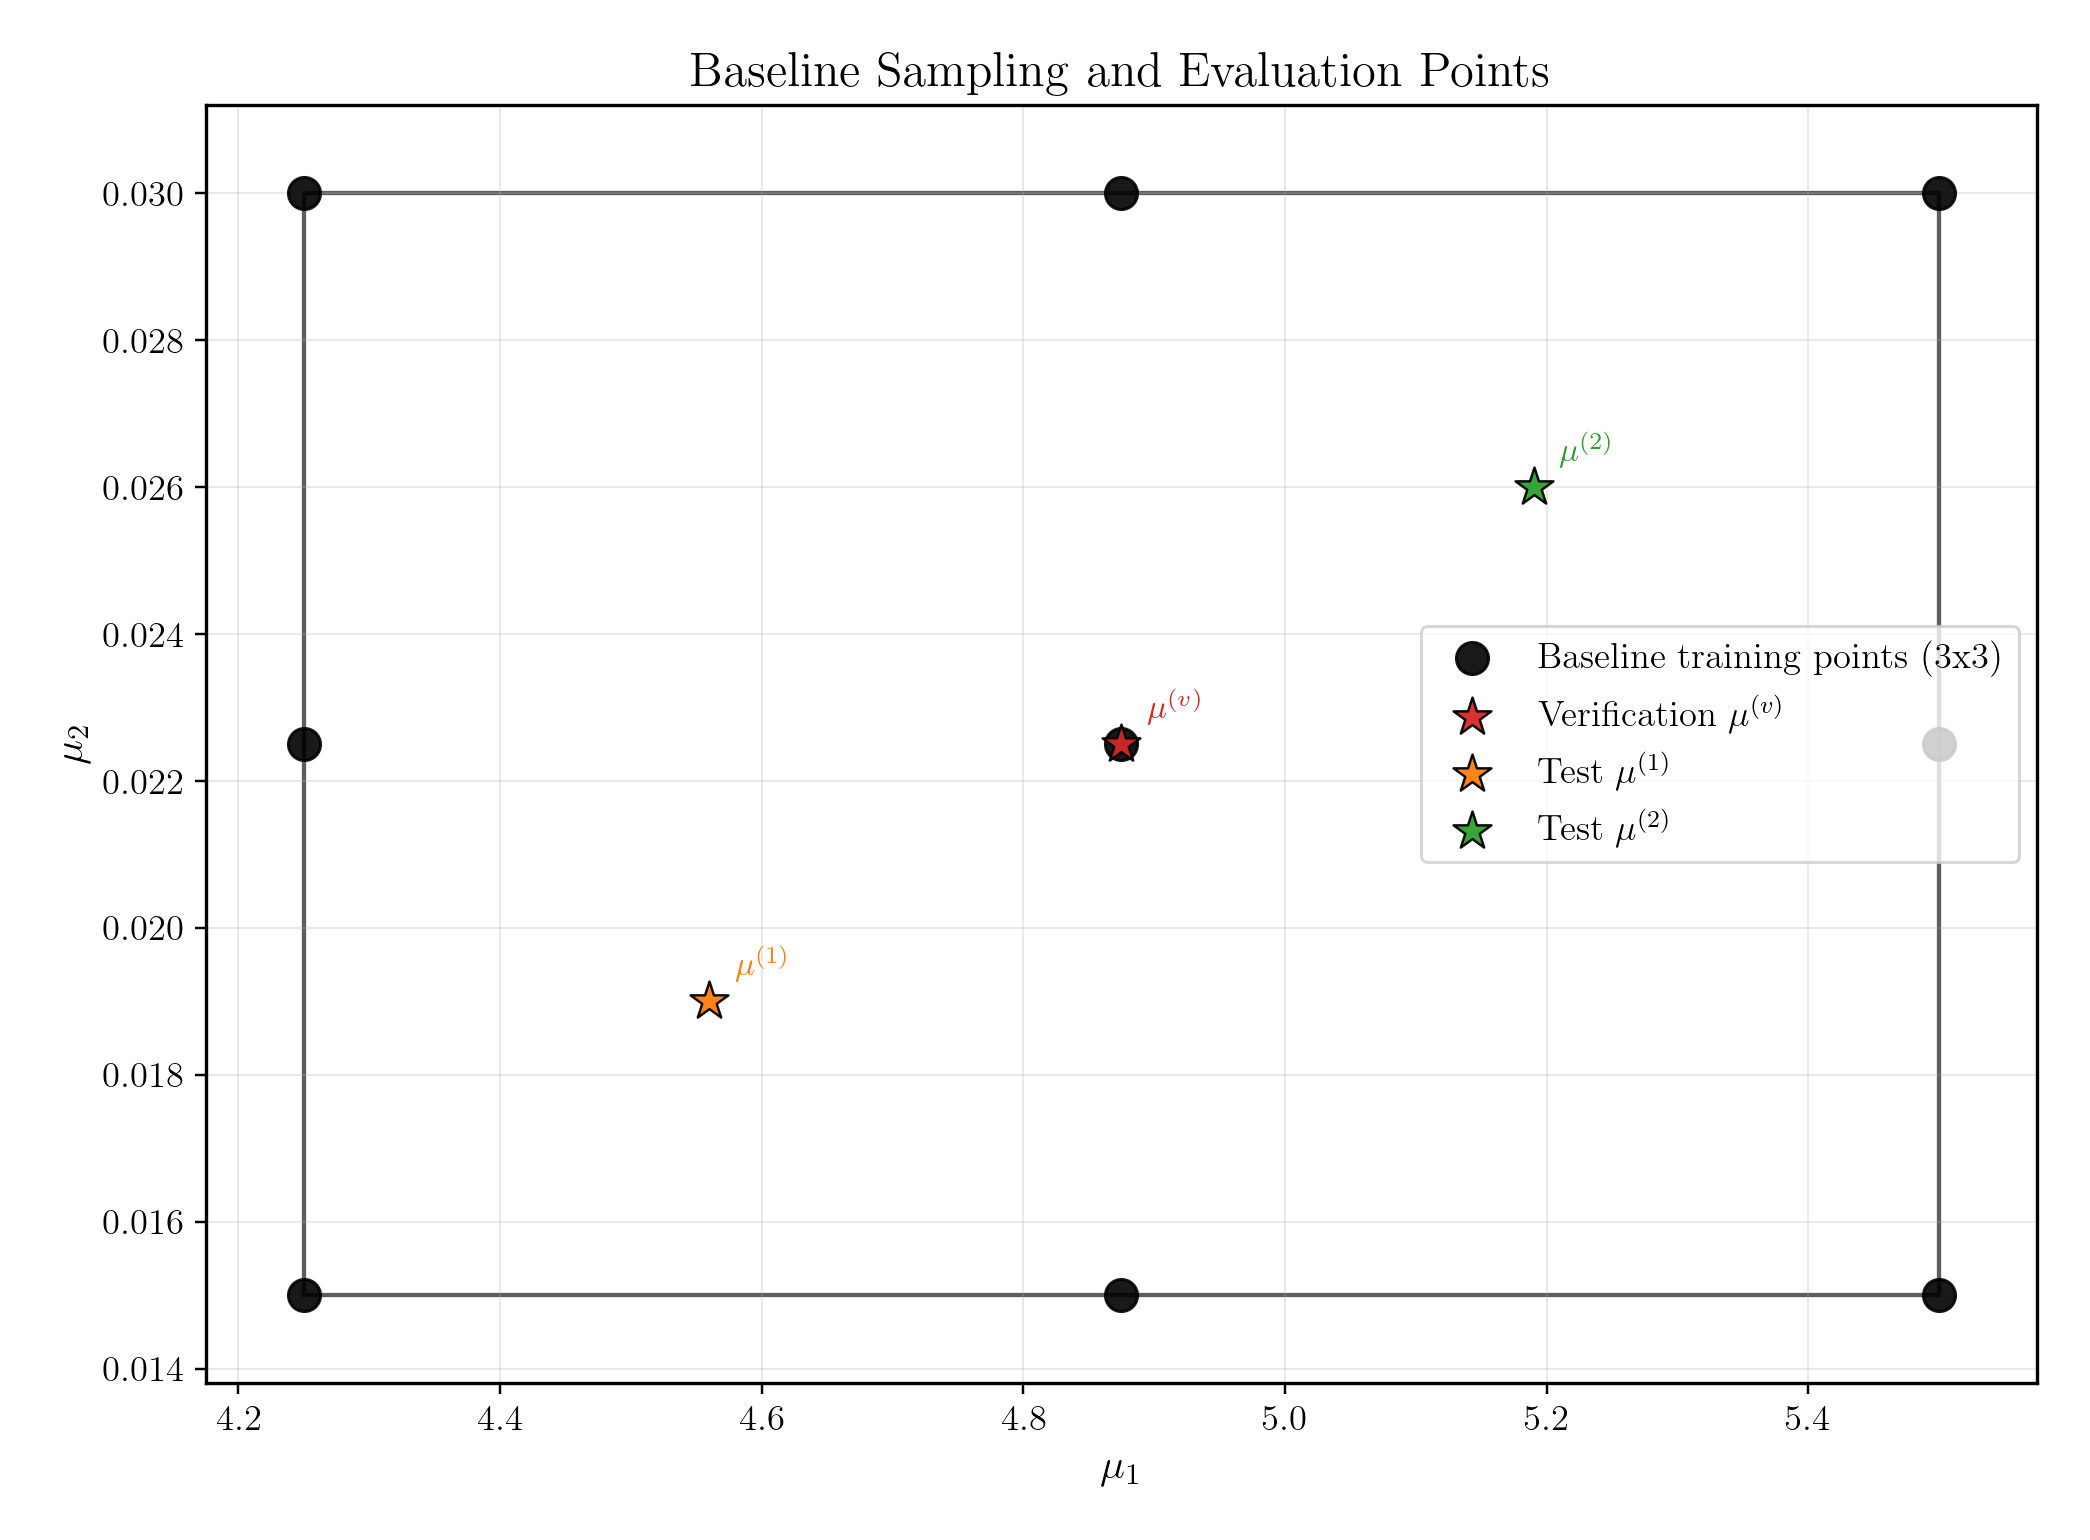
\includegraphics[width=0.62\textwidth]{Figures/stage1_sampling_points.png}
\vspace{-0.5em}
\caption{Baseline $3\times3$ structured sampling points in $\mathcal D$ (black circles) and evaluation points $\bm\mu^{(v)}$, $\bm\mu^{(1)}$, $\bm\mu^{(2)}$ (colored stars).}
\label{fig:param_sampling}
\end{figure}

% =========================================================
% =========================================================
% =========================================================
\section{PROM workflow and evaluation on the $250\times250$ mesh}
\label{sec:prom_250_workflow}

\paragraph{Scope.}
All results in this section are based on the $250\times250$ mesh only ($N=125{,}000$). The nonlinear maps are trained from PROM-generated reduced trajectories and evaluated online with PROM only. The HPROM/ECSW route remains available in the implementation and is described in the methodological section, but it is not used in the quantitative comparisons reported below. We do not include oracle diagnostics in this version.

\paragraph{End-to-end pipeline.}
We follow the sequence below:
\begin{enumerate}
\item Build a POD basis from HDM snapshots at $9$ equidistant training parameters (uniform $3\times3$ grid on $\mathcal D$).
\item Retain $n_{\mathrm{tot}}=151$ modes using tolerance-based truncation ($\texttt{pod\_tol}=10^{-4}$), with $n=10$ primary and $\bar n=141$ secondary modes.
\item Build the linear reduced model in the full space $\mathbf V_{\mathrm{tot}}\in\mathbb R^{N\times151}$ and generate the Stage-2 coefficient dataset from PROM trajectories:
\[
\mathbf q_N^{\mathrm{PROM}}(t;\bm\mu)=\begin{bmatrix}\mathbf q(t;\bm\mu)\\ \bar{\mathbf q}(t;\bm\mu)\end{bmatrix}.
\]
\item Train four nonlinear maps from this dataset: Case 1, Case 2, Case 3, and the purely data-driven map $\mathcal G(\bm\mu,t)\approx \mathbf q_N^{\mathrm{PROM}}$.
\item Evaluate all models at three points (verification point first, then two off-grid test points):
\[
\bm\mu^{(v)}=(4.875,0.0225),\qquad
\bm\mu^{(1)}=(4.56,0.019),\qquad
\bm\mu^{(2)}=(5.19,0.026),
\]
using PROM online solves.
\item Enrichment stage: add $20$ LHS points, regenerate PROM coefficients $\mathbf q_N^{\mathrm{PROM}}$ (no HDM reruns), retrain the same four maps, and re-evaluate at the same three points.
\end{enumerate}

\paragraph{Data-driven baseline (very brief).}
The data-driven model is a direct regression
\[
\mathcal G:(\bm\mu,t)\mapsto \mathbf q_N(t;\bm\mu),
\]
that predicts all $n_{\mathrm{tot}}$ coefficients from parameter and time only. It does not run an online LSPG/Gauss--Newton solve.

\paragraph{ANN architecture and optimization setup.}
For the production runs in this report (Case~1, Case~2, Case~3, and data-driven), we use the same MLP core architecture with ELU activations:
\[
32 \rightarrow 64 \rightarrow 128 \rightarrow 256 \rightarrow 256,
\]
followed by an output layer of task-dependent size. Training uses AdamW with learning rate $10^{-3}$, weight decay $10^{-6}$, early stopping (patience $120$), and fixed seed $42$.
Case~1, Case~2, Case~3, and data-driven use batch size $128$.
For Case~2 with $n=20$, we also tested several alternative architectures/activations and optimizer settings; the best run in our tests still used this same baseline architecture.

\paragraph{Dataset sizes.}
Baseline Stage-3 training uses $M=4509$ samples ($9\times501$).  
Enriched Stage-3 training uses $M=14529$ samples ($(9+20)\times501$).

\paragraph{POD spectrum.}
Figure~\ref{fig:stage1_svd_decay_250} reports the singular-value decay used to select the POD truncation at tolerance $\texttt{pod\_tol}=10^{-4}$. Figure~\ref{fig:stage1_svd_decay_250_first50} shows a zoom on the first 50 modes.

\begin{figure}[H]
\centering

\includegraphics[width=0.68\textwidth]{Figures/stage1_pod_singular_value_decay.png}
\caption{Singular value decay of the centered HDM snapshot matrix on the $250\times250$ mesh (Stage 1 POD).}
\label{fig:stage1_svd_decay_250}
\end{figure}

\begin{figure}[H]
\centering
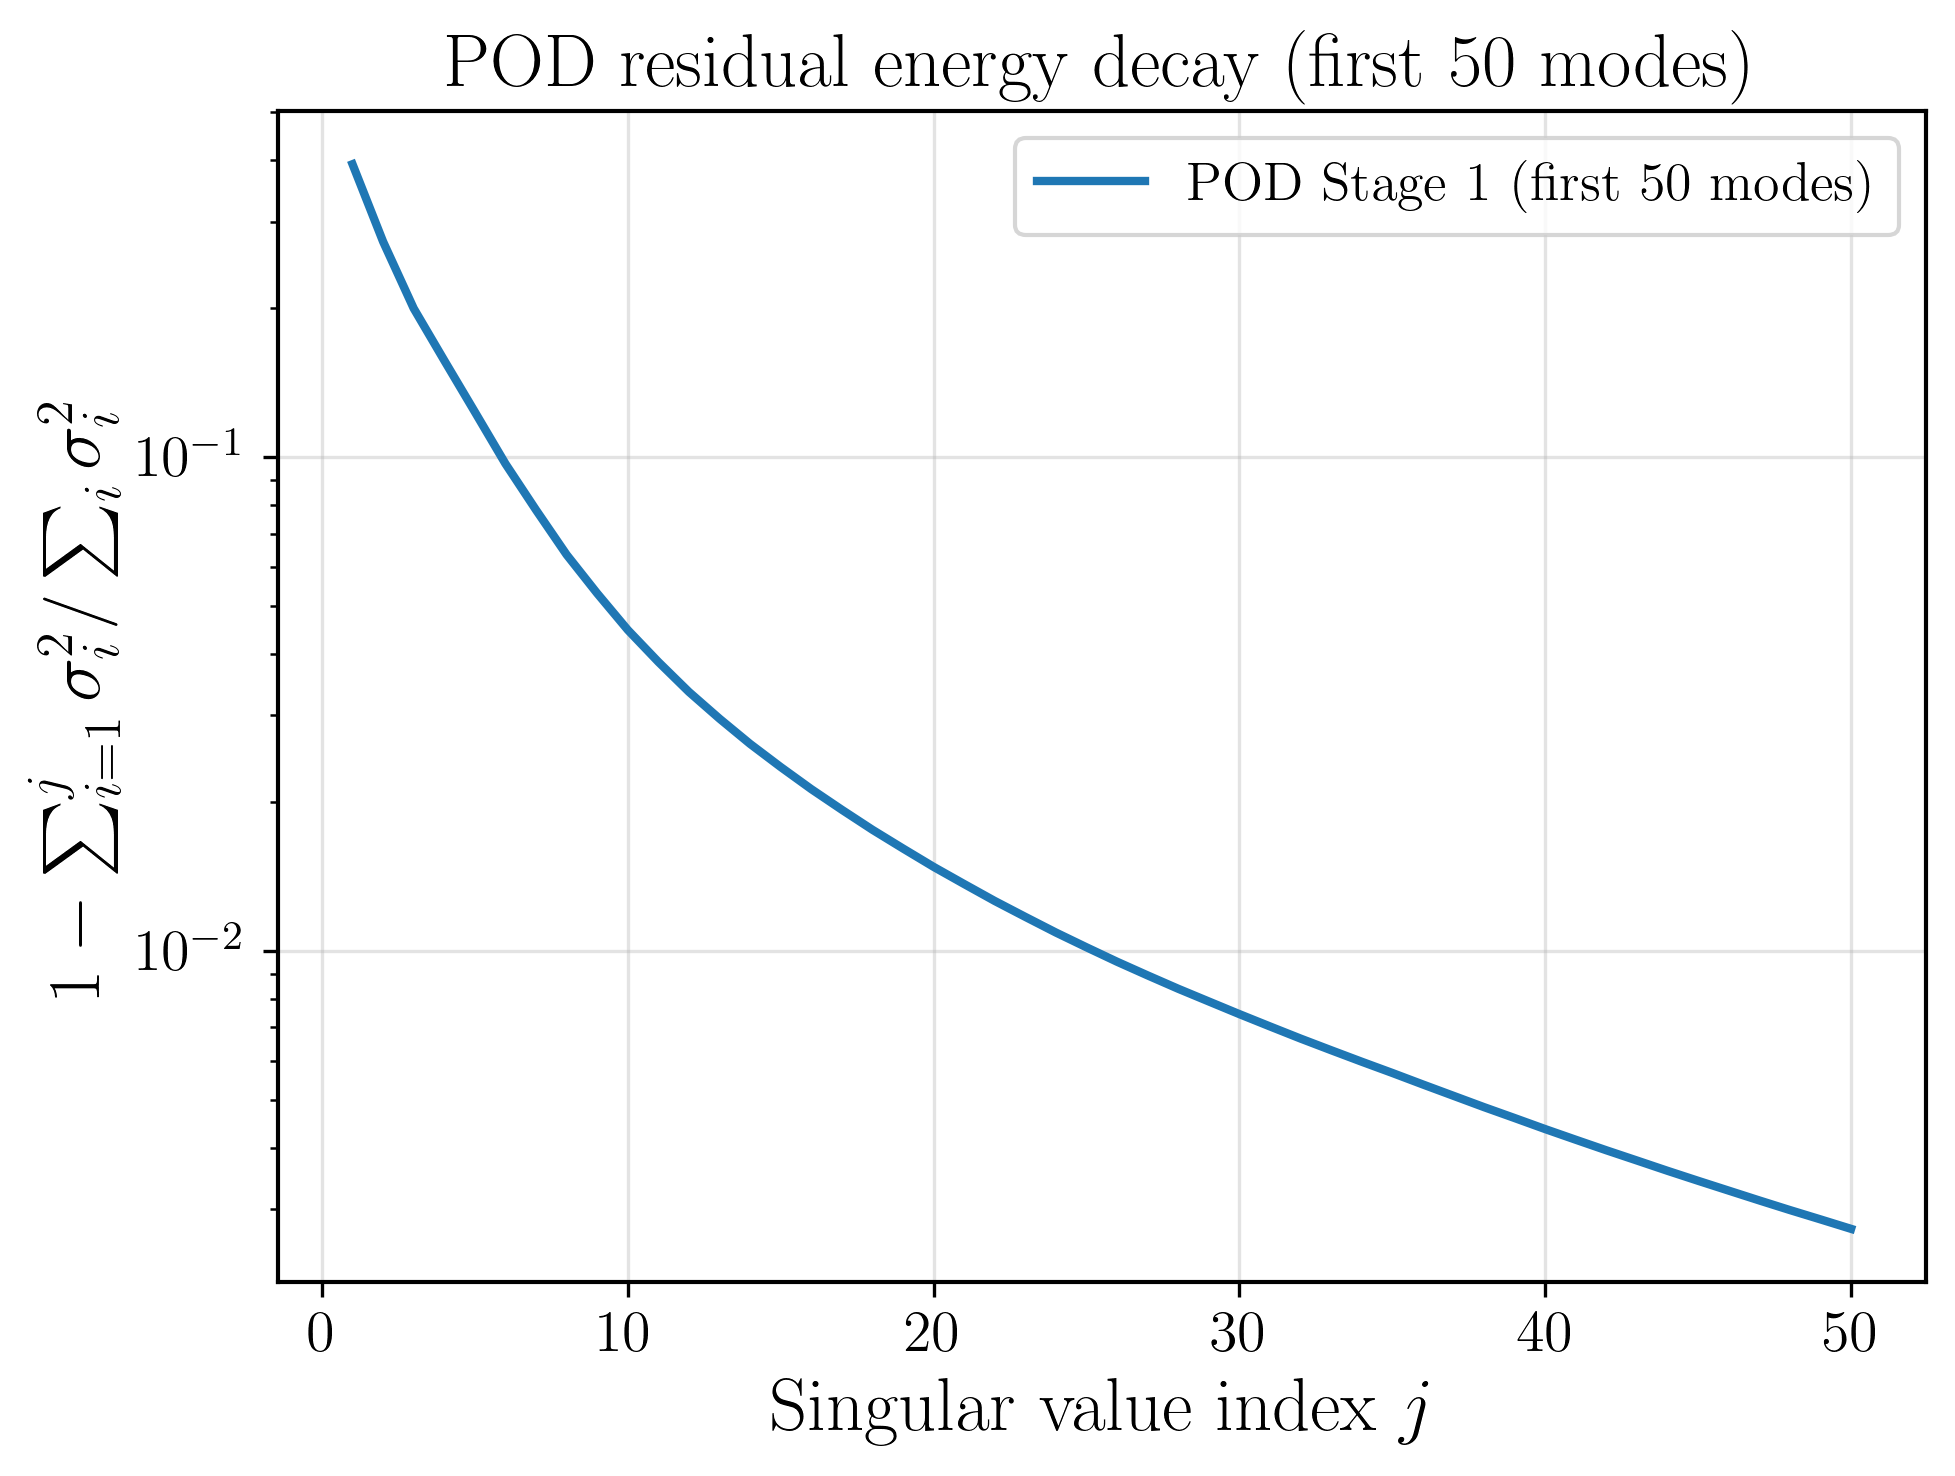
\includegraphics[width=0.68\textwidth]{Figures/stage1_pod_singular_value_decay_first50.png}
\caption{Zoom of the Stage 1 POD singular-value decay for the first 50 modes on the $250\times250$ mesh.}
\label{fig:stage1_svd_decay_250_first50}
\end{figure}

\paragraph{Sampling used for enrichment.}
Figure~\ref{fig:stage2_sampling_lhs20} shows the original $3\times3$ training points together with the $20$ LHS enrichment points used to build the enriched PROM coefficient dataset, plus the three evaluation points.

\begin{figure}[H]
\centering
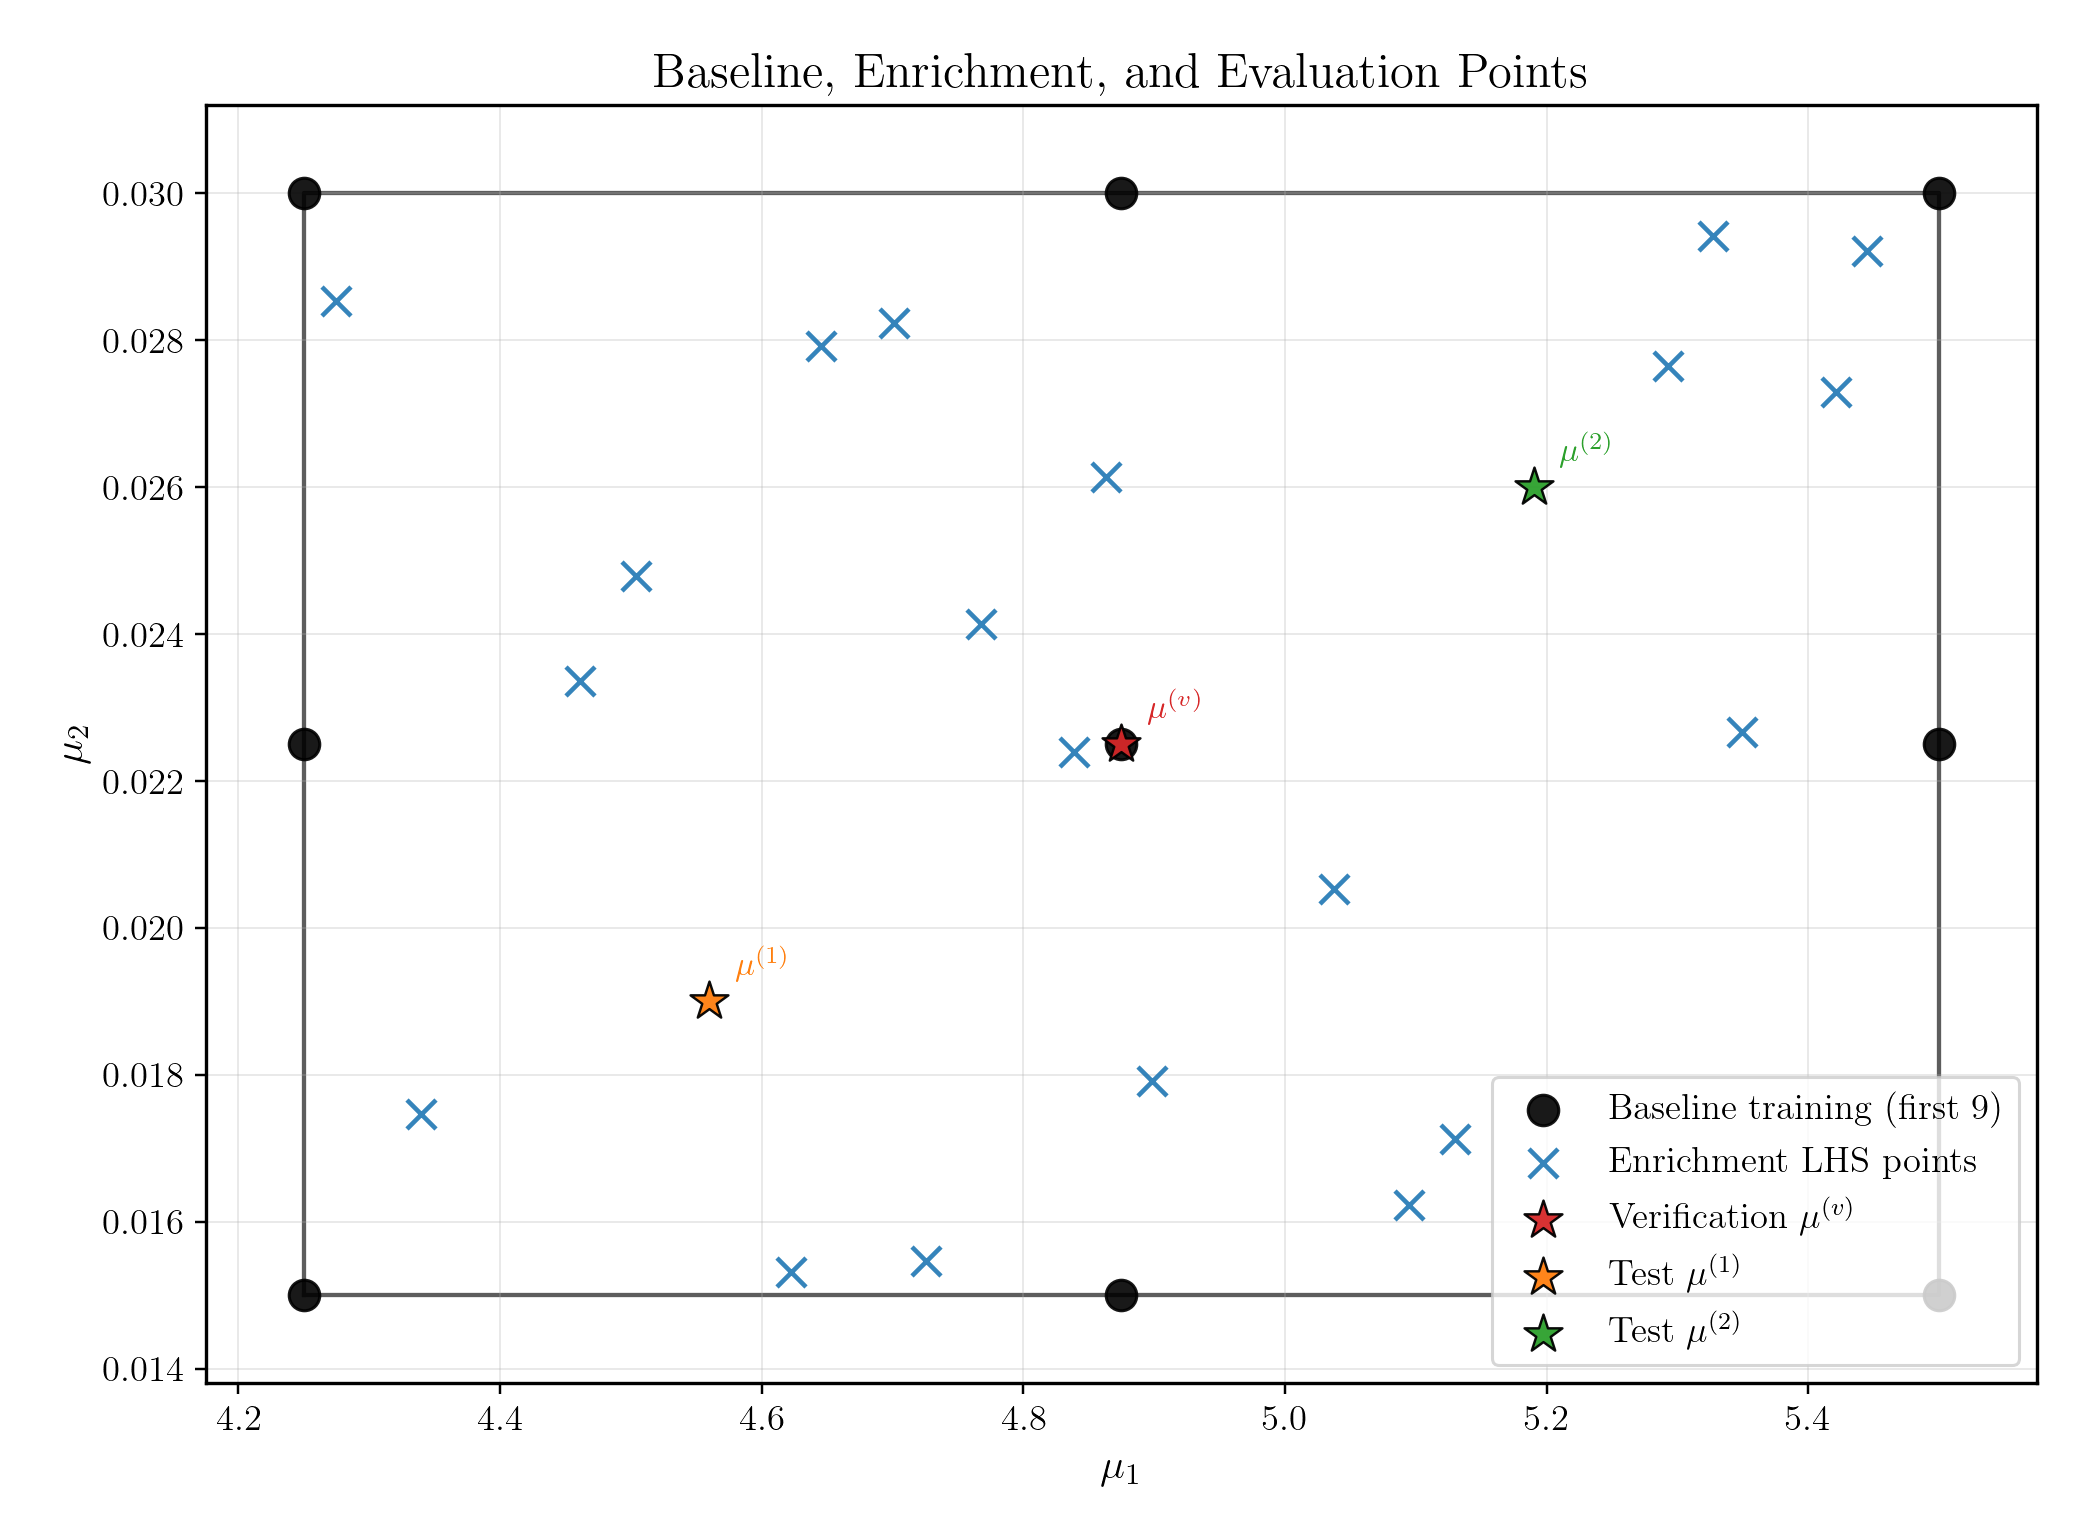
\includegraphics[width=0.70\textwidth]{Figures/stage2_sampling_points.png}
\caption{Baseline training points (9 equidistant points), enrichment points (20 LHS samples), and evaluation points $\bm\mu^{(v)}$, $\bm\mu^{(1)}$, $\bm\mu^{(2)}$ over $\mathcal D$.}
\label{fig:stage2_sampling_lhs20}
\end{figure}

% =========================================================
\subsection{Baseline models (9-point training dataset)}
\label{sec:baseline_prom_250}

Table~\ref{tab:baseline_prom_250} reports trajectory-level relative errors and online runtimes for the PROM-consistent campaign. We include a linear $n_{\mathrm{tot}}$-PROM reference, the three ANN closure variants, the Case~2 Petrov-Galerkin (PG) variant, a Case~2 run with $n=20$, and the purely data-driven model. The HPROM backend remains available in the codebase, but it is not used for the quantitative tables in this section.
In all result tables below, ``Case~2 + PG'' denotes the \emph{Case~2 with enriched residual testing} formulation introduced above.
The trajectory-level relative error is computed against the HDM trajectory:
\[
\mathrm{RelErr}(\bm\mu)
=
100\,
\frac{\left\|\mathbf U_{\mathrm{HDM}}(\bm\mu)-\mathbf U_{\mathrm{model}}(\bm\mu)\right\|_F}
{\left\|\mathbf U_{\mathrm{HDM}}(\bm\mu)\right\|_F},
\]
where $\mathbf U\in\mathbb R^{N\times (N_t+1)}$ stacks the state snapshots in time.

\begin{table}[H]
\centering
\caption{Baseline PROM results on $250\times250$ ($n_{\mathrm{tot}}=151$), including Case~2 variants for $n=10$ and $n=20$.}
\label{tab:baseline_prom_250}
\resizebox{\textwidth}{!}{
\begin{tabular}{lcccccc}
\hline
Method & RelErr$(\bm\mu^{(v)})$ [\%] & RelErr$(\bm\mu^{(1)})$ [\%] & RelErr$(\bm\mu^{(2)})$ [\%] & Time$(\bm\mu^{(v)})$ [s] & Time$(\bm\mu^{(1)})$ [s] & Time$(\bm\mu^{(2)})$ [s] \\
\hline
Linear PROM ($n_{\mathrm{tot}}=151$) & 0.410 & 0.450 & 0.463 & 921.943 & 871.356 & 913.506 \\
Case 1 ANN ($\bar{\mathbf q}=\mathcal N(\mathbf q)$) & 0.708 & 0.716 & 1.103 & 148.840 & 147.333 & 149.762 \\
Case 2 ANN ($\bar{\mathbf q}=\mathcal M(\bm\mu,t)$) & 0.874 & 1.224 & 1.507 & 90.985 & 92.647 & 91.022 \\
Case 2 ANN + PG (enriched residual testing) & 0.793 & 1.202 & 1.223 & 409.562 & 409.104 & 406.139 \\
Case 2 ANN ($n=20$, $\bar n=131$) & 0.652 & 6.502 & 3.755 & 146.334 & 141.090 & 141.372 \\
Case 3 ANN ($\bar{\mathbf q}=\mathcal H(\mathbf q,\bm\mu,t)$) & 0.655 & 0.765 & 0.788 & 149.478 & 149.438 & 151.618 \\
Data-driven ($\mathbf q_N=\mathcal G(\bm\mu,t)$) & 0.874 & 1.832 & 1.580 & 0.005 & 0.005 & 0.005 \\
\hline
\end{tabular}
}
\end{table}

% =========================================================
\subsection{Enriched models (9+20 training dataset)}
\label{sec:enriched_prom_250}

For enrichment, we augment the baseline $9$ trajectories with $20$ LHS trajectories and retrain all four nonlinear maps. Table~\ref{tab:enriched_prom_250} reports PROM results at the same three points, including the Case~2 PG and $n=20$ variants. The linear $n_{\mathrm{tot}}$-PROM row is unchanged and is included for reference.

\begin{table}[H]
\centering
\caption{Enriched PROM results on $250\times250$ (trained with $9+20$ trajectories, $n_{\mathrm{tot}}=151$), including Case~2 variants for $n=10$ and $n=20$.}
\label{tab:enriched_prom_250}
\resizebox{\textwidth}{!}{
\begin{tabular}{lcccccc}
\hline
Method & RelErr$(\bm\mu^{(v)})$ [\%] & RelErr$(\bm\mu^{(1)})$ [\%] & RelErr$(\bm\mu^{(2)})$ [\%] & Time$(\bm\mu^{(v)})$ [s] & Time$(\bm\mu^{(1)})$ [s] & Time$(\bm\mu^{(2)})$ [s] \\
\hline
Linear PROM ($n_{\mathrm{tot}}=151$) & 0.410 & 0.450 & 0.463 & 921.943 & 871.356 & 913.506 \\
Case 1 ANN (enriched) & 0.681 & 0.561 & 0.922 & 156.034 & 156.136 & 156.006 \\
Case 2 ANN (enriched) & 0.894 & 0.962 & 0.875 & 91.416 & 91.013 & 90.763 \\
Case 2 ANN + PG (enriched) & 0.685 & 0.754 & 0.714 & 413.579 & 411.149 & 415.588 \\
Case 2 ANN ($n=20$, $\bar n=131$, enriched) & 0.499 & 0.550 & 0.548 & 140.796 & 141.836 & 141.215 \\
Case 3 ANN (enriched) & 0.473 & 0.517 & 0.532 & 156.095 & 155.333 & 165.269 \\
Data-driven (enriched) & 0.860 & 0.928 & 0.896 & 0.006 & 0.006 & 0.006 \\
\hline
\end{tabular}
}
\end{table}

% =========================================================
\subsection{Runtime and speed-up reporting}
\label{sec:speedup_prom_250}

Using measured HDM wall-clock times
\begin{align}
t_{\mathrm{HDM}}(\bm\mu^{(v)}) &= 7.542\times10^2\ \mathrm{s},\\
t_{\mathrm{HDM}}(\bm\mu^{(1)}) &= 7.507\times10^2\ \mathrm{s},\\
t_{\mathrm{HDM}}(\bm\mu^{(2)}) &= 7.577\times10^2\ \mathrm{s},
\end{align}
where $t_{\mathrm{HDM}}(\bm\mu^{(v)})$ is taken as a credible interpolation-level reference between the two measured off-grid HDM times.
we define speed-up at each test point as
\[
S_m(\bm\mu)=\frac{t_{\mathrm{HDM}}(\bm\mu)}{t_m(\bm\mu)}.
\]
Table~\ref{tab:speedup_prom_250} reports baseline and enriched speed-ups for all three points.

\begin{table}[H]
\centering
\caption{PROM speed-up factors relative to HDM at the three reported points.}
\label{tab:speedup_prom_250}
\resizebox{\textwidth}{!}{
\begin{tabular}{lcccccc}
\hline
Method & Baseline $S(\bm\mu^{(v)})$ & Baseline $S(\bm\mu^{(1)})$ & Baseline $S(\bm\mu^{(2)})$ & Enriched $S(\bm\mu^{(v)})$ & Enriched $S(\bm\mu^{(1)})$ & Enriched $S(\bm\mu^{(2)})$ \\
\hline
Linear PROM ($n_{\mathrm{tot}}=151$) & 0.82 & 0.86 & 0.83 & 0.82 & 0.86 & 0.83 \\
Case 1 ANN & 5.07 & 5.10 & 5.06 & 4.83 & 4.81 & 4.86 \\
Case 2 ANN & 8.29 & 8.10 & 8.32 & 8.25 & 8.25 & 8.35 \\
Case 2 ANN + PG & 1.84 & 1.84 & 1.87 & 1.82 & 1.83 & 1.82 \\
Case 2 ANN ($n=20$) & 5.15 & 5.32 & 5.36 & 5.36 & 5.29 & 5.37 \\
Case 3 ANN & 5.05 & 5.02 & 5.00 & 4.83 & 4.83 & 4.58 \\
Data-driven & $1.44\times10^{5}$ & $1.43\times10^{5}$ & $1.46\times10^{5}$ & $1.20\times10^{5}$ & $1.18\times10^{5}$ & $1.34\times10^{5}$ \\
\hline
\end{tabular}
}
\end{table}

\paragraph{Note.}
The data-driven runtime is pure ANN inference time and does not include a reduced nonlinear solve. Therefore, its speed-up values are not directly comparable to PROM nonlinear-solve timings.

% =========================================================
\subsection{Effect of enrichment}
\label{sec:enrichment_effect_250}

Define relative error reduction from baseline to enriched as
\[
\Delta e = 100\frac{e_{\mathrm{base}}-e_{\mathrm{enriched}}}{e_{\mathrm{base}}}.
\]
Table~\ref{tab:enrichment_gain_250} reports baseline and enriched errors together with $\Delta e$ at all three points.

\begin{table}[H]
\centering
\caption{Baseline vs enriched trajectory errors and relative reduction (\%) on $250\times250$. Positive $\Delta e$ indicates improvement.}
\label{tab:enrichment_gain_250}
\resizebox{\textwidth}{!}{
\begin{tabular}{lccccccccc}
\hline
Method & $e_{\text{base}}(\bm\mu^{(v)})$ [\%] & $e_{\text{enr}}(\bm\mu^{(v)})$ [\%] & $\Delta e(\bm\mu^{(v)})$ [\%] & $e_{\text{base}}(\bm\mu^{(1)})$ [\%] & $e_{\text{enr}}(\bm\mu^{(1)})$ [\%] & $\Delta e(\bm\mu^{(1)})$ [\%] & $e_{\text{base}}(\bm\mu^{(2)})$ [\%] & $e_{\text{enr}}(\bm\mu^{(2)})$ [\%] & $\Delta e(\bm\mu^{(2)})$ [\%] \\
\hline
Linear PROM ($n_{\mathrm{tot}}=151$) & 0.410 & 0.410 & 0.00 & 0.450 & 0.450 & 0.00 & 0.463 & 0.463 & 0.00 \\
Case 1 ANN & 0.708 & 0.681 & 3.75 & 0.716 & 0.561 & 21.68 & 1.103 & 0.922 & 16.43 \\
Case 2 ANN & 0.874 & 0.894 & -2.36 & 1.224 & 0.962 & 21.39 & 1.507 & 0.875 & 41.96 \\
Case 2 ANN + PG & 0.793 & 0.685 & 13.56 & 1.202 & 0.754 & 37.28 & 1.223 & 0.714 & 41.59 \\
Case 2 ANN ($n=20$) & 0.652 & 0.499 & 23.56 & 6.502 & 0.550 & 91.54 & 3.755 & 0.548 & 85.40 \\
Case 3 ANN & 0.655 & 0.473 & 27.75 & 0.765 & 0.517 & 32.45 & 0.788 & 0.532 & 32.44 \\
Data-driven & 0.874 & 0.860 & 1.67 & 1.832 & 0.928 & 49.35 & 1.580 & 0.896 & 43.28 \\
\hline
\end{tabular}
}
\end{table}

\paragraph{Remark and practical takeaway.}
In this PROM-consistent campaign, the linear $n_{\mathrm{tot}}$-PROM remains the most accurate reference but at the highest online cost. For Case~2, the PG variant improves all three enriched-point errors relative to the standard Case~2 row, but with a substantially larger runtime (speed-up near $1.8\times$ only). For the $n=20$ Case~2 split, the baseline model is accurate at the verification point but degrades strongly at the two off-grid points; after enrichment, those two off-grid errors drop markedly.

% =========================================================
\subsection{Interpretation of the Case 2 $n=20$ behavior}
\label{sec:case2_n20_interp}

At first glance, Case~2 with $n=20$ may seem as if it should be easier than $n=10$, because the ANN output size drops from $\bar n=141$ to $\bar n=131$. However, in our setup, the main difficulty is not only output dimension; it is generalization of the map $(\bm\mu,t)\mapsto\bar{\mathbf q}$ across the domain with only $9$ baseline trajectories.

For Case~2 specifically, $\bar{\mathbf q}$ does not depend on the online state $\mathbf q$. This means the model cannot correct truncated content based on instantaneous reduced-state deviations during the solve. Changing from $n=10$ to $n=20$ changes the retained/truncated split and therefore changes which dynamics must be represented by the standalone map $\mathcal M(\bm\mu,t)$. With limited baseline data, this can degrade off-grid robustness even if the output dimension is smaller.

This is consistent with the observed pattern: baseline $n=20$ performs well at the central verification point but poorly at off-grid points, while enrichment ($9+20$ trajectories) restores good behavior.

% =========================================================
\subsection{Coefficient-space error analysis and source decomposition}
\label{sec:coeff_errors_250}

Unless stated otherwise, the coefficient-space diagnostics below correspond to the standard $n=10$ closure models (without the PG Case~2 variant and without the $n=20$ split).

To isolate reduced-coordinate effects, we use the linear $n_{\mathrm{tot}}$-PROM coefficients as reference:
\[
\mathbf q^{\mathrm{ref}}(t;\bm\mu) := \mathbf q_N^{\mathrm{Linear\ PROM}}(t;\bm\mu).
\]
For each model $m\in\{\text{Case~1, Case~2, Case~3, Data-driven}\}$, with coefficients $\mathbf q^{(m)}$, we define per-mode trajectory errors
\[
E_i^{\mathrm{abs}}(m;\bm\mu)=\left\|q_i^{\mathrm{ref}}-q_i^{(m)}\right\|_2,\qquad
E_i^{\mathrm{rel}}(m;\bm\mu)=\frac{E_i^{\mathrm{abs}}(m;\bm\mu)}{\left\|q_i^{\mathrm{ref}}\right\|_2}.
\]
Here, the norm is taken over time and $i$ indexes POD coefficients.

We split reduced coordinates as $\mathbf q_N=[\mathbf q;\bar{\mathbf q}]$, where $\mathbf q$ is retained and $\bar{\mathbf q}$ is truncated (implementation aliases: $\mathbf q_p,\mathbf q_s$). We define
\textbf{Source~1} (retained-coordinate mismatch, i.e. mismatch in the solved LSPG unknown $\mathbf q$) and total truncated mismatch as
\[
\mathbf e_q^{(m)}:=\mathbf q^{\mathrm{ref}}-\mathbf q^{(m)},
\qquad
\eta_q^{(m)}:=\frac{\|\mathbf e_q^{(m)}\|_F}{\|\mathbf q^{\mathrm{ref}}\|_F},
\]
\[
\mathbf e_{\bar q,\mathrm{tot}}^{(m)}:=\bar{\mathbf q}^{\mathrm{ref}}-\bar{\mathbf q}^{(m)},
\qquad
\eta_{\bar q}^{(m)}:=\frac{\|\mathbf e_{\bar q,\mathrm{tot}}^{(m)}\|_F}{\|\bar{\mathbf q}^{\mathrm{ref}}\|_F}.
\]
Table~\ref{tab:coeff_primary_secondary_summary} summarizes means over the three reported points.

\begin{table}[H]
\centering
\caption{Mean relative coefficient errors (\%) over $\bm\mu^{(v)},\bm\mu^{(1)},\bm\mu^{(2)}$, using linear $n_{\mathrm{tot}}$-PROM coefficients as reference.}
\label{tab:coeff_primary_secondary_summary}
\begin{tabular}{lcccc}
\hline
Method & Baseline $\eta_q$ [\%] & Baseline $\eta_{\bar q}$ [\%] & Enriched $\eta_q$ [\%] & Enriched $\eta_{\bar q}$ [\%] \\
\hline
Case 1 ANN & 0.80 & 7.55 & 0.67 & 6.08 \\
Case 2 ANN & 1.54 & 9.88 & 1.62 & 4.49 \\
Case 3 ANN & 0.71 & 6.40 & 0.29 & 2.69 \\
Data-driven & 2.04 & 11.69 & 1.08 & 7.46 \\
\hline
\end{tabular}
\end{table}

\paragraph{Error-source decomposition for closure models.}
For Cases~1--3, the truncated-coordinate error $\mathbf e_{\bar q,\mathrm{tot}}$ can be decomposed as follows.
There is no independent ``Source~1'' term for $\bar{\mathbf q}$ because $\bar{\mathbf q}$ is not solved as an independent unknown in these closure models. Source~1 acts on $\bar{\mathbf q}$ only indirectly through Source~3 when the closure depends on $\mathbf q$ (Cases~1 and~3). For Case~2, Source~3 is identically absent.

\textbf{Case 1:}
\[
\mathbf e_{\bar q,\mathrm{tot}}^{(1)}
=\bar{\mathbf q}^{\mathrm{ref}}-\bar{\mathbf q}^{(1)}
=\underbrace{\left(\bar{\mathbf q}^{\mathrm{ref}}-\mathcal N(\mathbf q^{\mathrm{ref}})\right)}_{\text{Source 2: map mismatch}}
+\underbrace{\left(\mathcal N(\mathbf q^{\mathrm{ref}})-\mathcal N(\mathbf q^{(1)})\right)}_{\text{Source 3: continuity / sensitivity}}.
\]
\textbf{Case 2:}
\[
\mathbf e_{\bar q,\mathrm{tot}}^{(2)}
=\bar{\mathbf q}^{\mathrm{ref}}-\bar{\mathbf q}^{(2)}
=\underbrace{\left(\bar{\mathbf q}^{\mathrm{ref}}-\mathcal M(\bm\mu,t)\right)}_{\text{Source 2: map mismatch}}.
\]
\textbf{Case 3:}
\[
\mathbf e_{\bar q,\mathrm{tot}}^{(3)}
=\bar{\mathbf q}^{\mathrm{ref}}-\bar{\mathbf q}^{(3)}
=\underbrace{\left(\bar{\mathbf q}^{\mathrm{ref}}-\mathcal H(\mathbf q^{\mathrm{ref}},\bm\mu,t)\right)}_{\text{Source 2: map mismatch}}
+\underbrace{\left(\mathcal H(\mathbf q^{\mathrm{ref}},\bm\mu,t)-\mathcal H(\mathbf q^{(3)},\bm\mu,t)\right)}_{\text{Source 3: continuity / sensitivity}}.
\]

For Cases~1 and~3, Source~3 can be interpreted as propagation of Source~1 through a $\mathbf q$-dependent closure. Under an additional regularity assumption, this propagation can be bounded: if the closure map is locally Lipschitz in the neighborhood visited by the trajectories, with local constant $L_{\mathcal F}$, then
\[
\|\text{Source 3}\|_F \le L_{\mathcal F}\,\|\mathbf e_q\|_F.
\]
This inequality is used here as a qualitative interpretation aid only: we do not estimate $L_{\mathcal F}$ from data, nor claim tightness of the bound. Source~1 is explicitly reported by $\eta_q$ in Table~\ref{tab:coeff_primary_secondary_summary}, while Table~\ref{tab:decomposition_summary_250} resolves Source~2 and Source~3 on truncated coefficients.

Table~\ref{tab:decomposition_summary_250} reports mean relative magnitudes of these terms over the three points.

\begin{table}[H]
\centering
\caption{Mean relative decomposition terms on truncated coefficients (\%) over $\bm\mu^{(v)},\bm\mu^{(1)},\bm\mu^{(2)}$.}
\label{tab:decomposition_summary_250}
\begin{tabular}{llccc}
\hline
Stage & Case & Source 2 [\%] & Source 3 [\%] & Total $\eta_{\bar q}$ [\%] \\
\hline
Baseline & Case 1 & 5.50 & 6.13 & 7.55 \\
Baseline & Case 2 & 9.88 & -- & 9.88 \\
Baseline & Case 3 & 3.58 & 5.84 & 6.40 \\
Enriched & Case 1 & 3.44 & 5.33 & 6.08 \\
Enriched & Case 2 & 4.49 & -- & 4.49 \\
Enriched & Case 3 & 2.40 & 1.68 & 2.69 \\
\hline
\end{tabular}
\end{table}

Figures~\ref{fig:coeff_abs_rel_baseline_verif} and~\ref{fig:coeff_abs_rel_enriched_verif} show per-index absolute and relative coefficient errors at the verification point, for baseline and enriched models, respectively. The corresponding plots for the two off-grid test points are reported in Appendix~\ref{app:coeff_curves_extra}.

\begin{figure}[H]
\centering
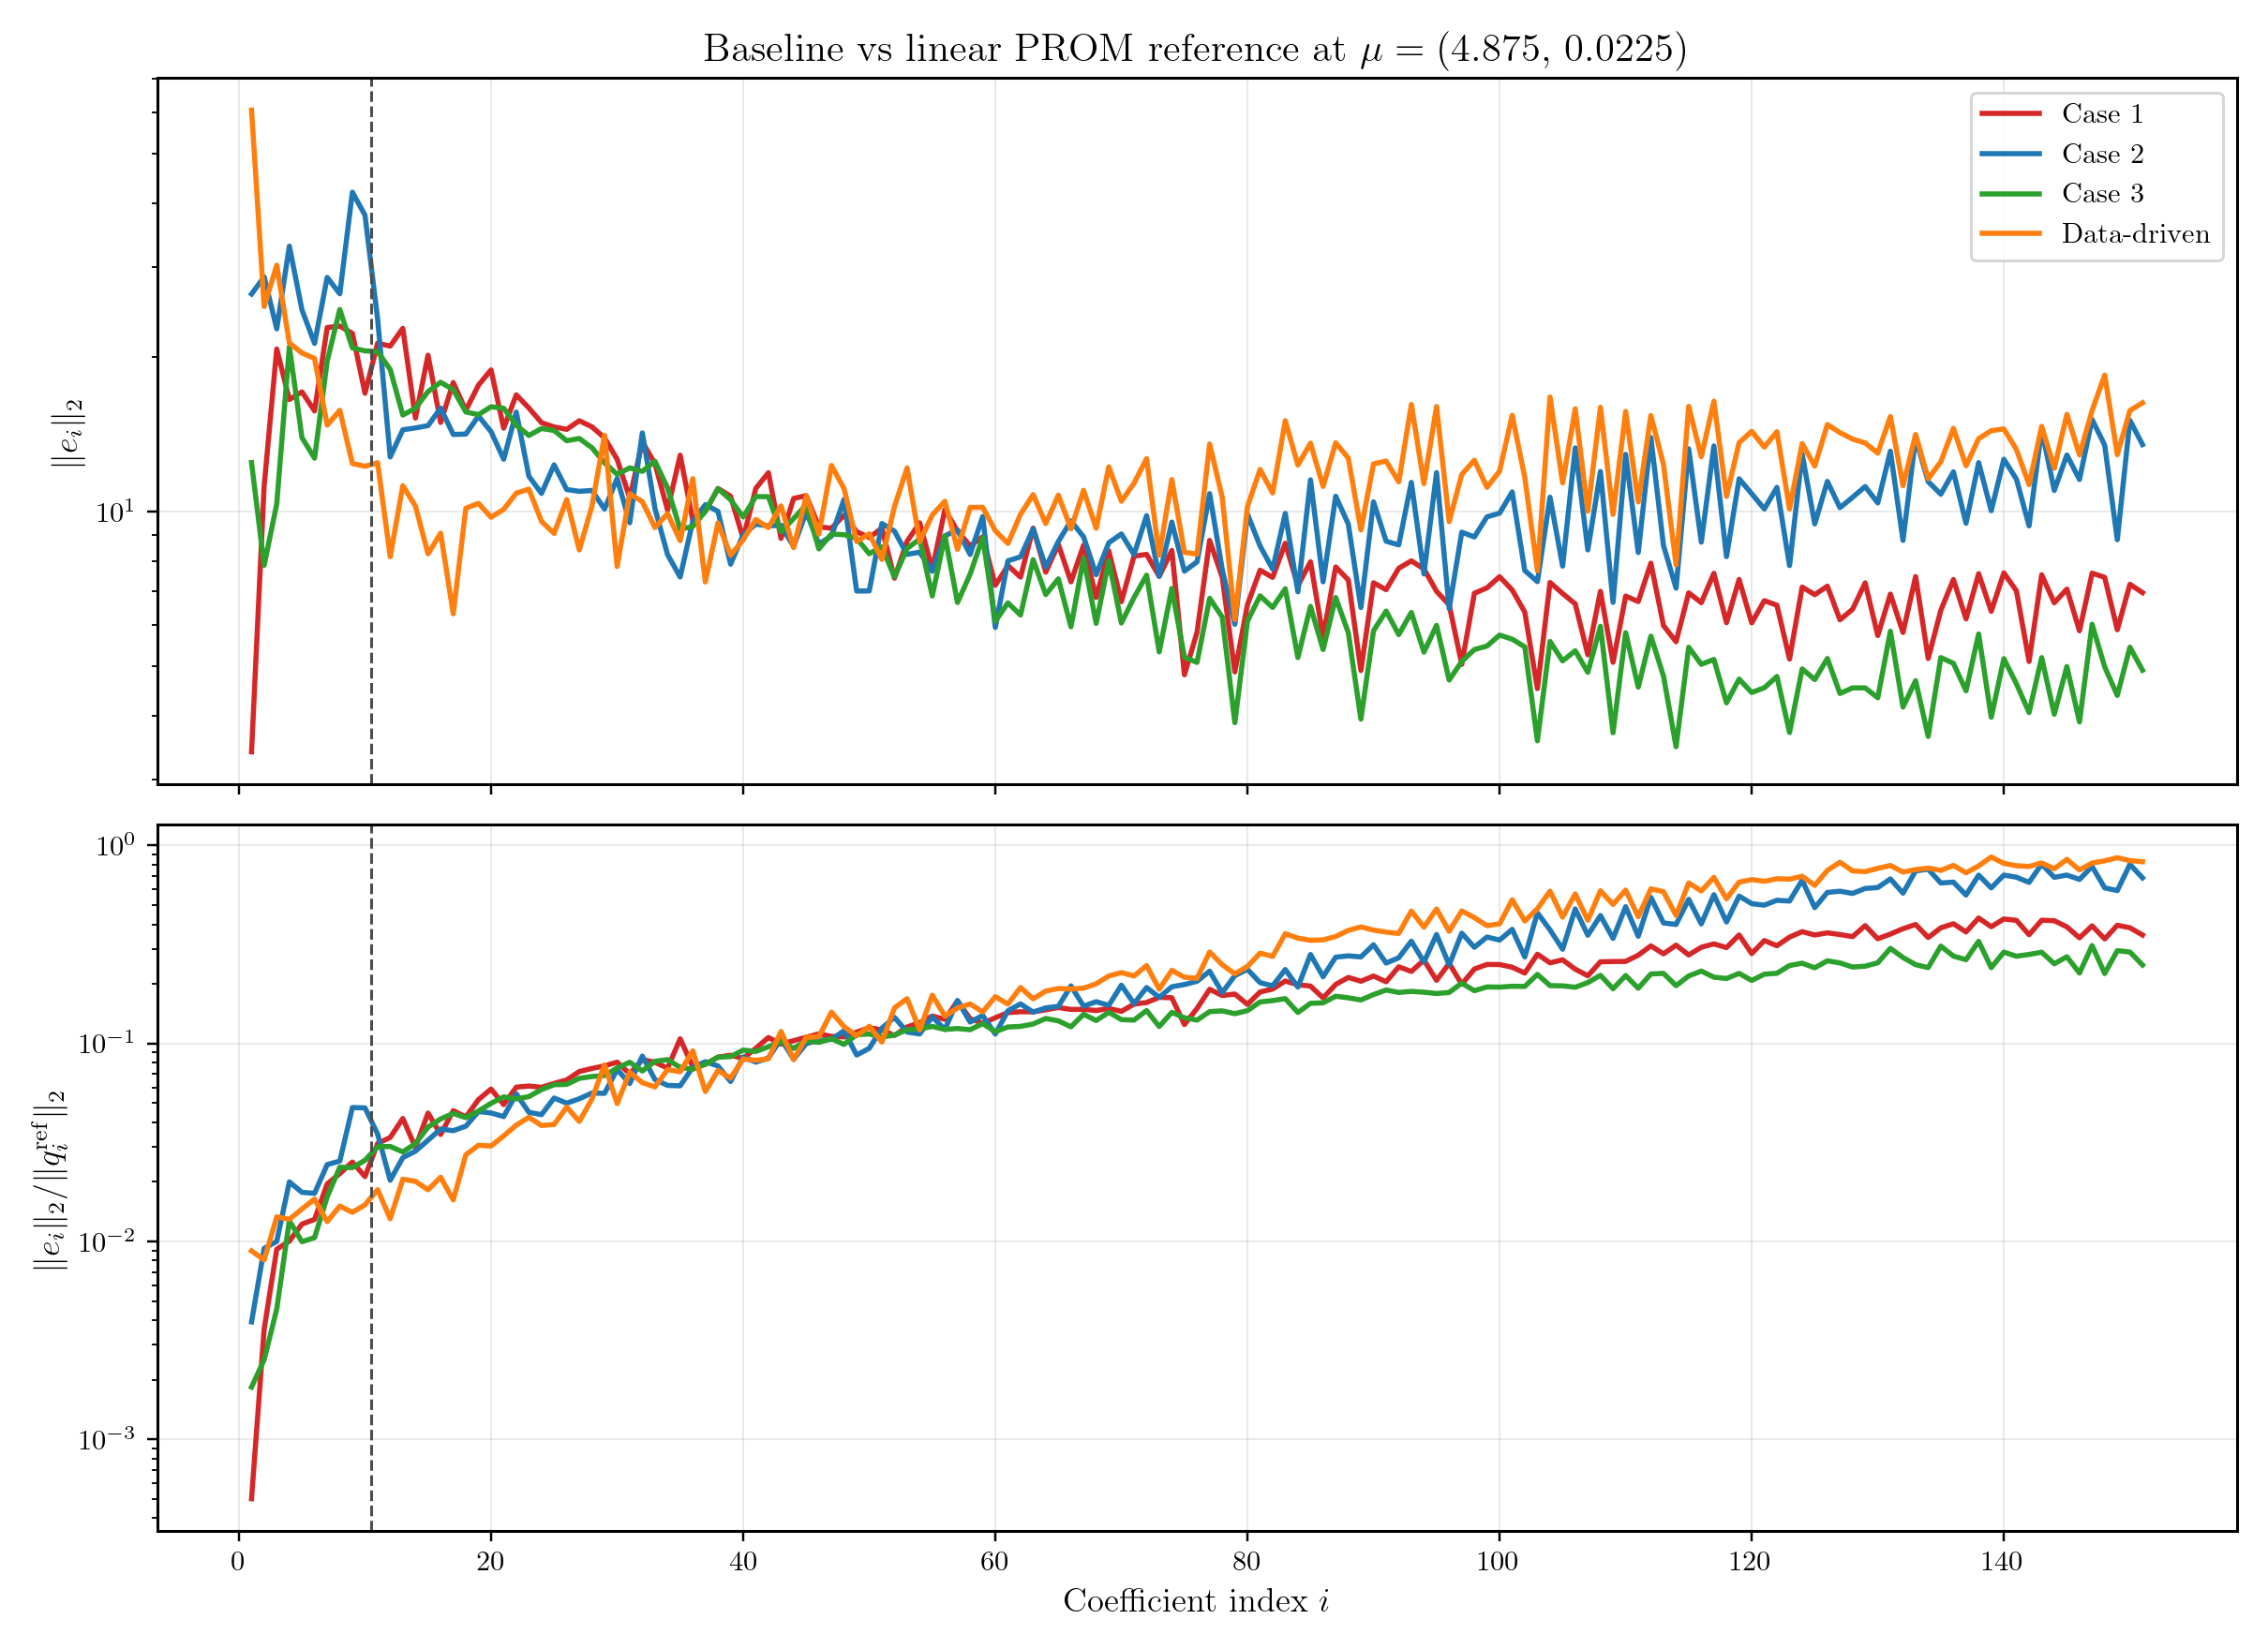
\includegraphics[width=0.94\textwidth]{Figures/coeff_errors/baseline_mu1_4.875_mu2_0.0225_coeff_abs_rel_vs_index.png}
\caption{Baseline stage: per-index absolute and relative coefficient errors vs linear $n_{\mathrm{tot}}$-PROM reference at $\bm\mu^{(v)}=(4.875,0.0225)$.}
\label{fig:coeff_abs_rel_baseline_verif}
\end{figure}

\begin{figure}[H]
\centering
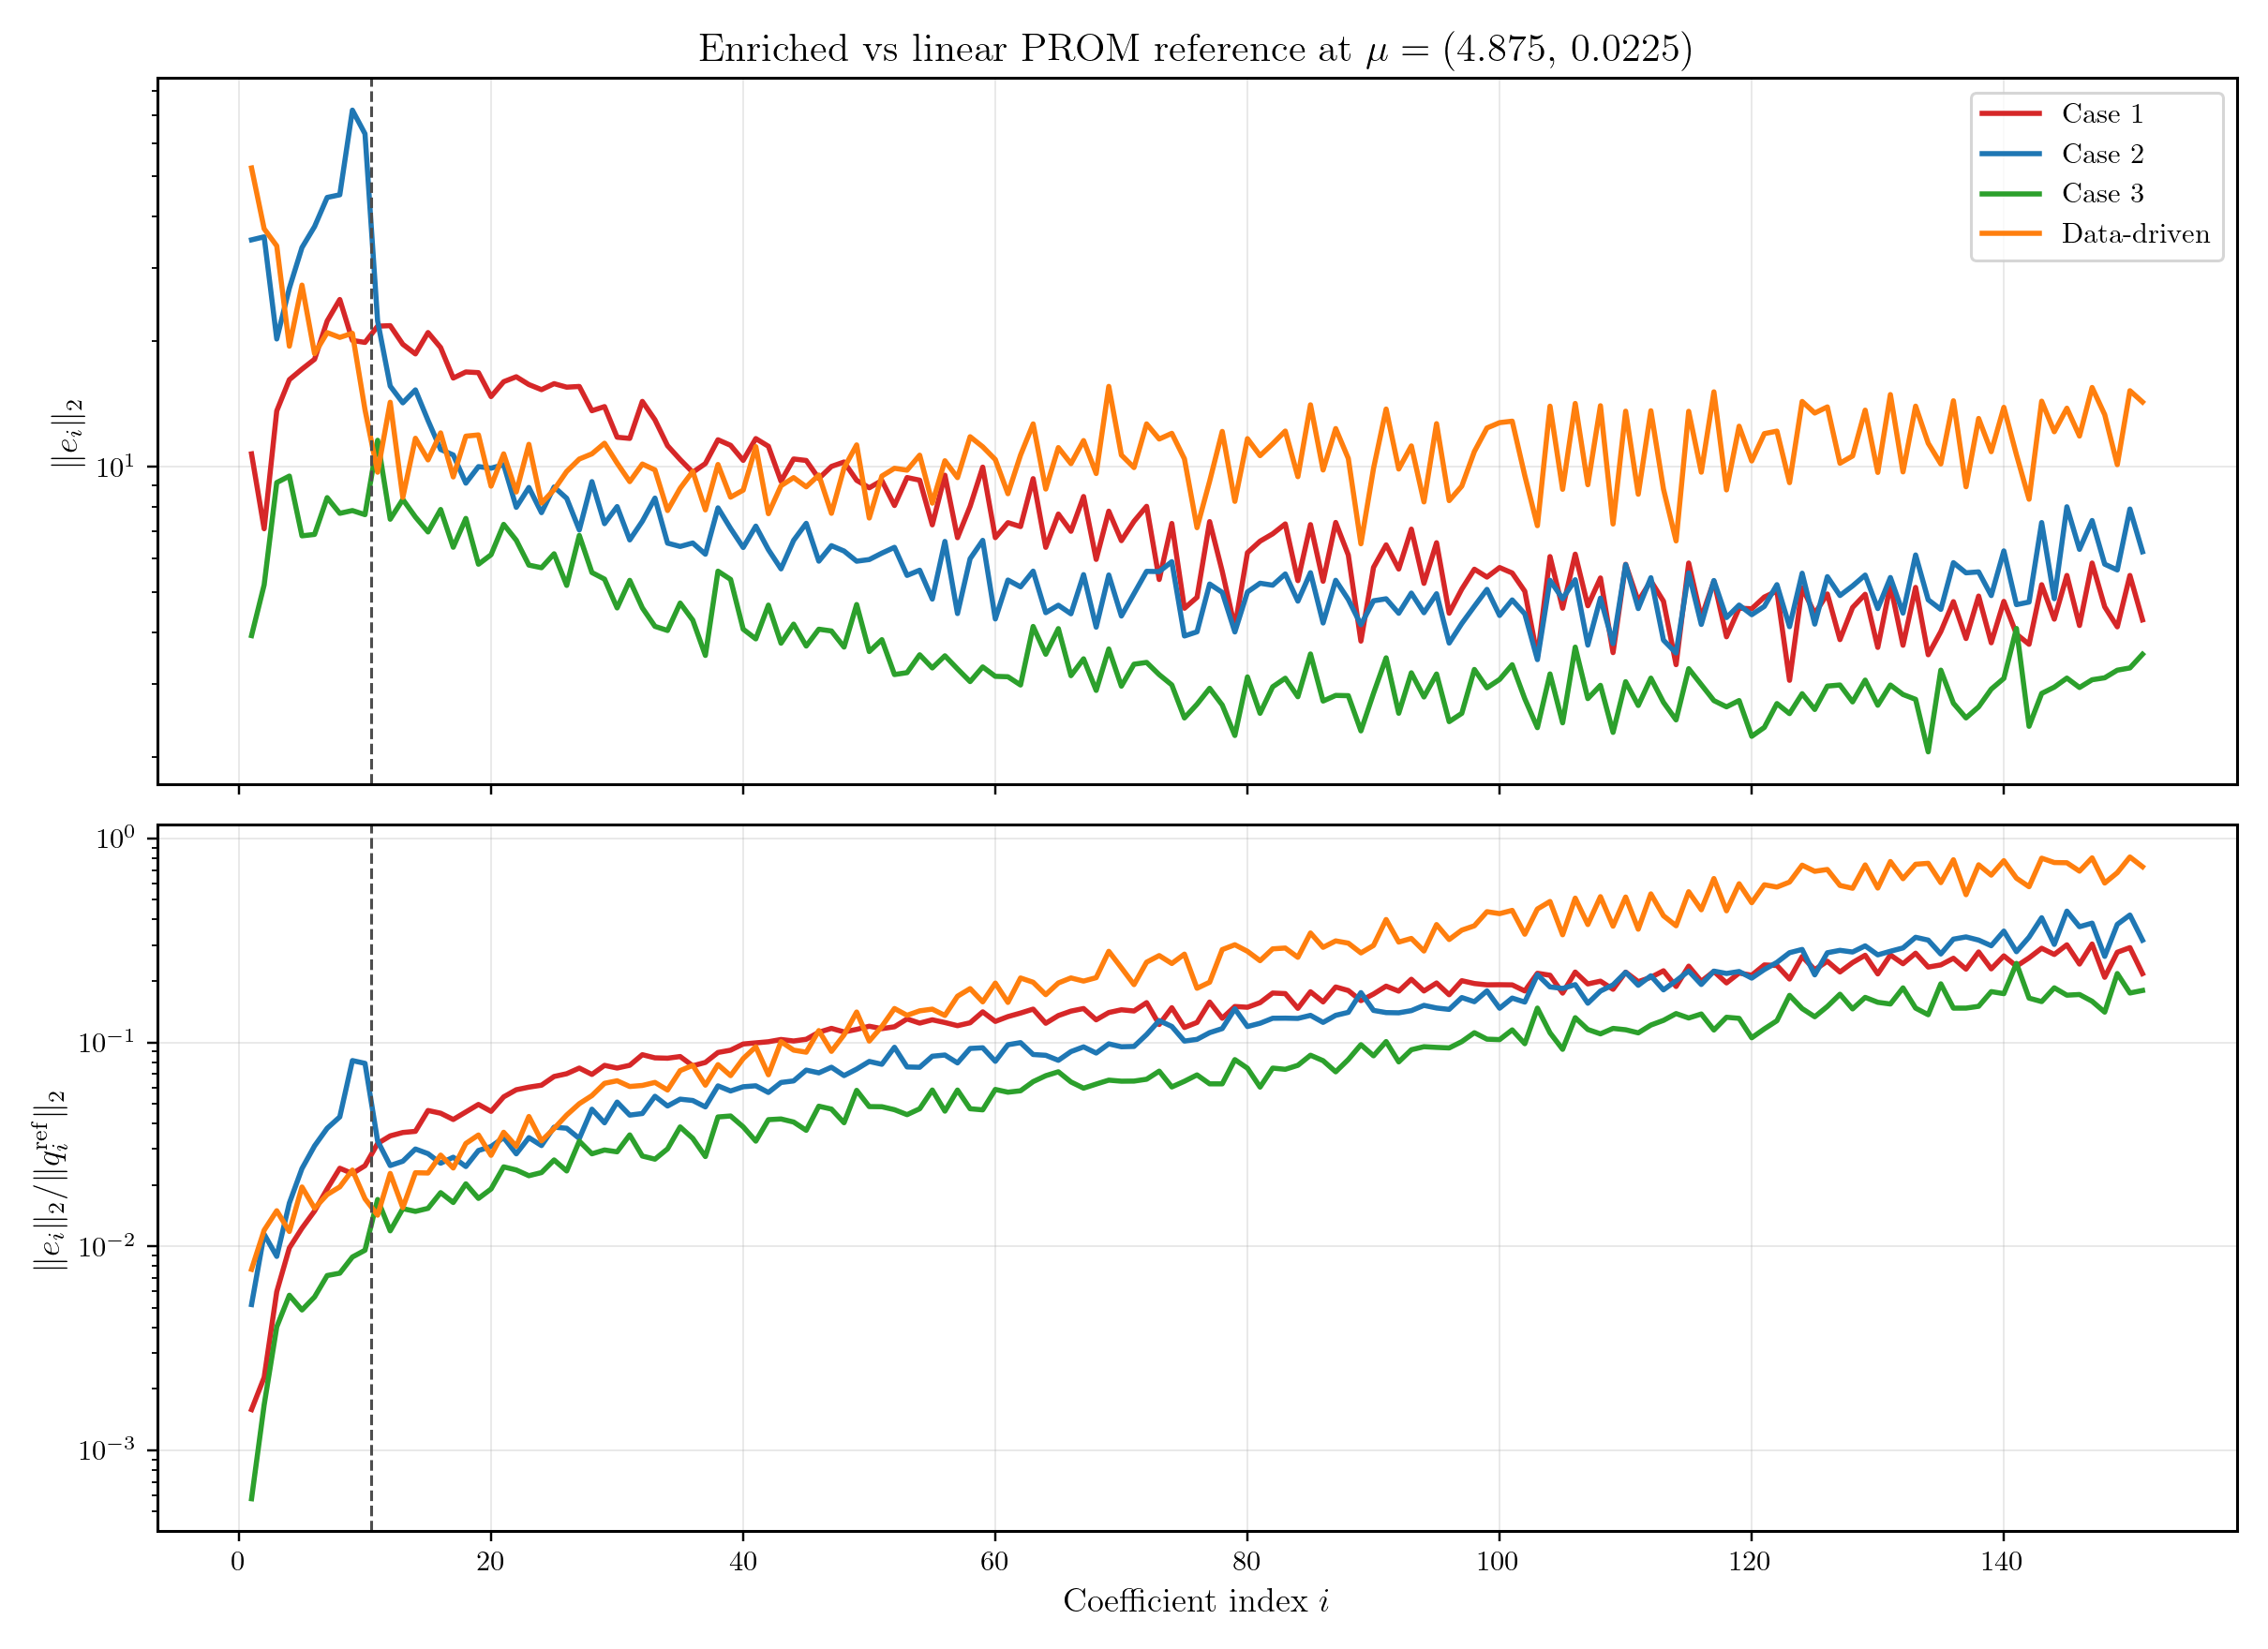
\includegraphics[width=0.94\textwidth]{Figures/coeff_errors/enriched_mu1_4.875_mu2_0.0225_coeff_abs_rel_vs_index.png}
\caption{Enriched stage: per-index absolute and relative coefficient errors vs linear $n_{\mathrm{tot}}$-PROM reference at $\bm\mu^{(v)}=(4.875,0.0225)$.}
\label{fig:coeff_abs_rel_enriched_verif}
\end{figure}

% =========================================================
\subsection{Qualitative comparison: HDM vs all models}
\label{sec:qual_prom_250}

Figures~\ref{fig:all_models_baseline_prom} and \ref{fig:all_models_enriched_prom} compare HDM (black) against Case~1 (red), Case~2 (blue), Case~3 (green), and data-driven (orange), ordered as $\bm\mu^{(v)}$, $\bm\mu^{(1)}$, and $\bm\mu^{(2)}$.

\begin{figure}[H]
\centering
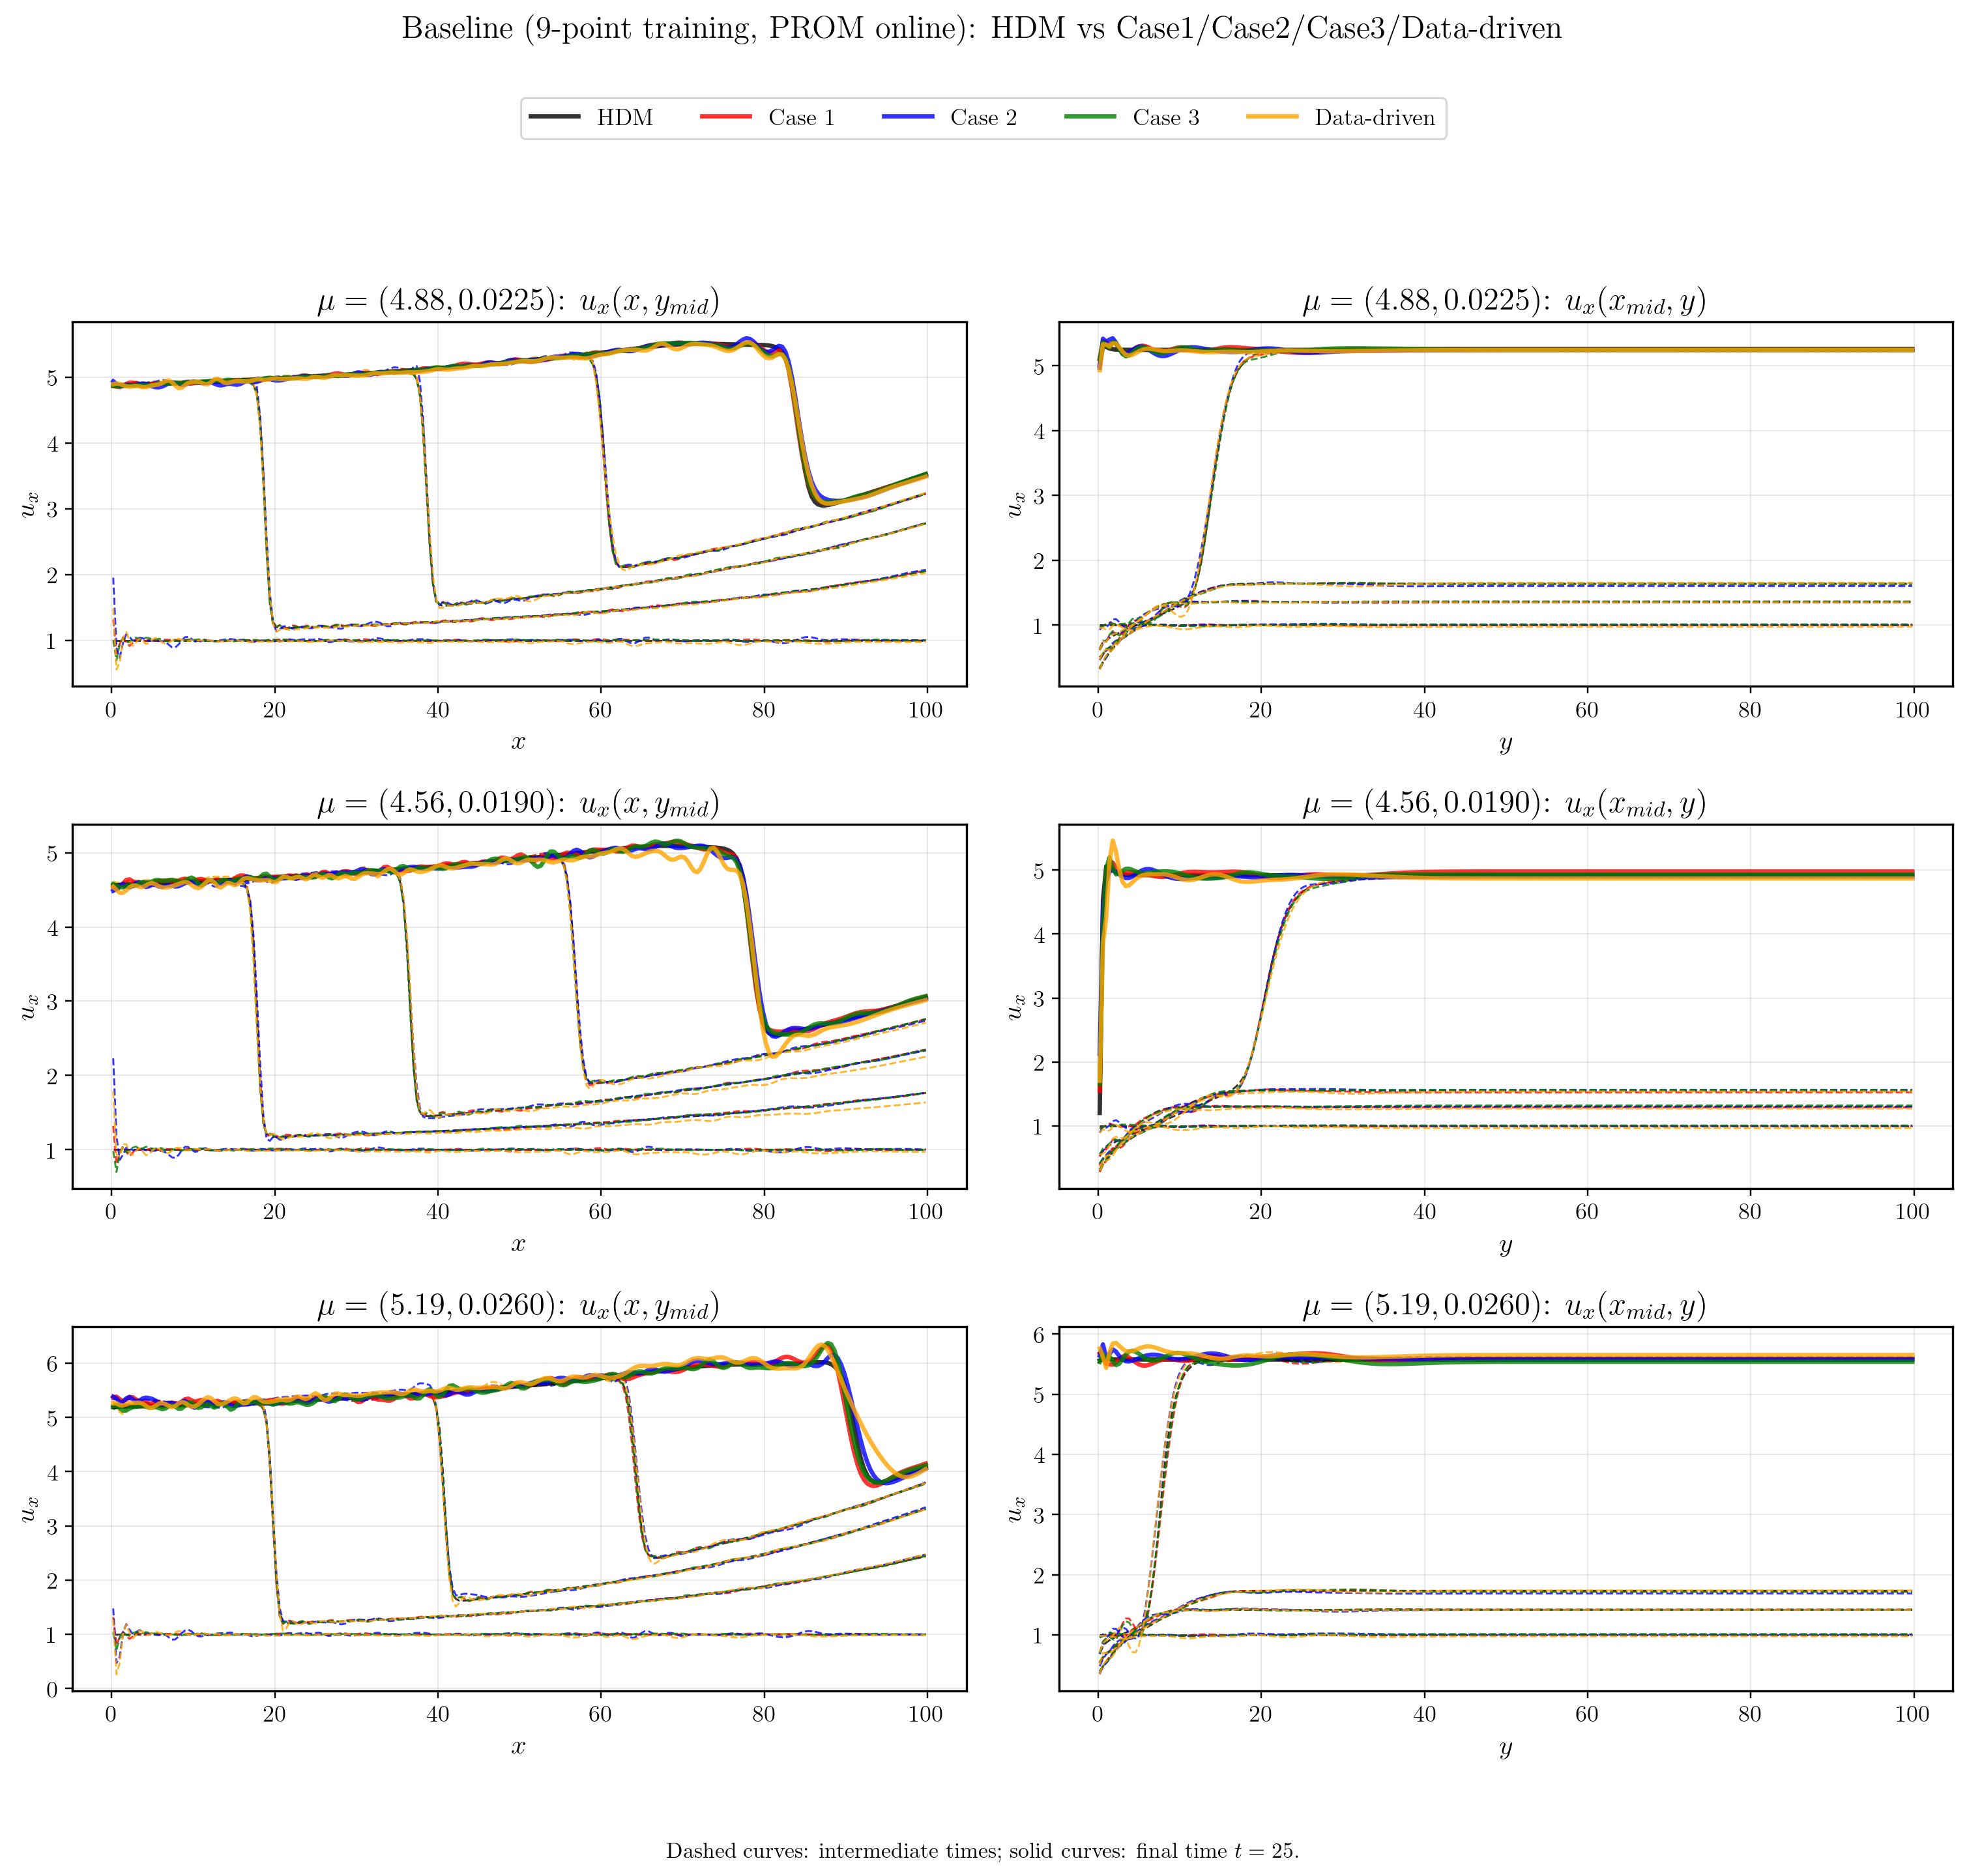
\includegraphics[width=0.98\textwidth]{Figures/baseline_prom_hdm_vs_all_models.png}
\caption{Baseline models, PROM online solve: HDM vs Case~1/2/3 and data-driven at $\bm\mu^{(v)}$, $\bm\mu^{(1)}$, and $\bm\mu^{(2)}$.}
\label{fig:all_models_baseline_prom}
\end{figure}

\begin{figure}[H]
\centering
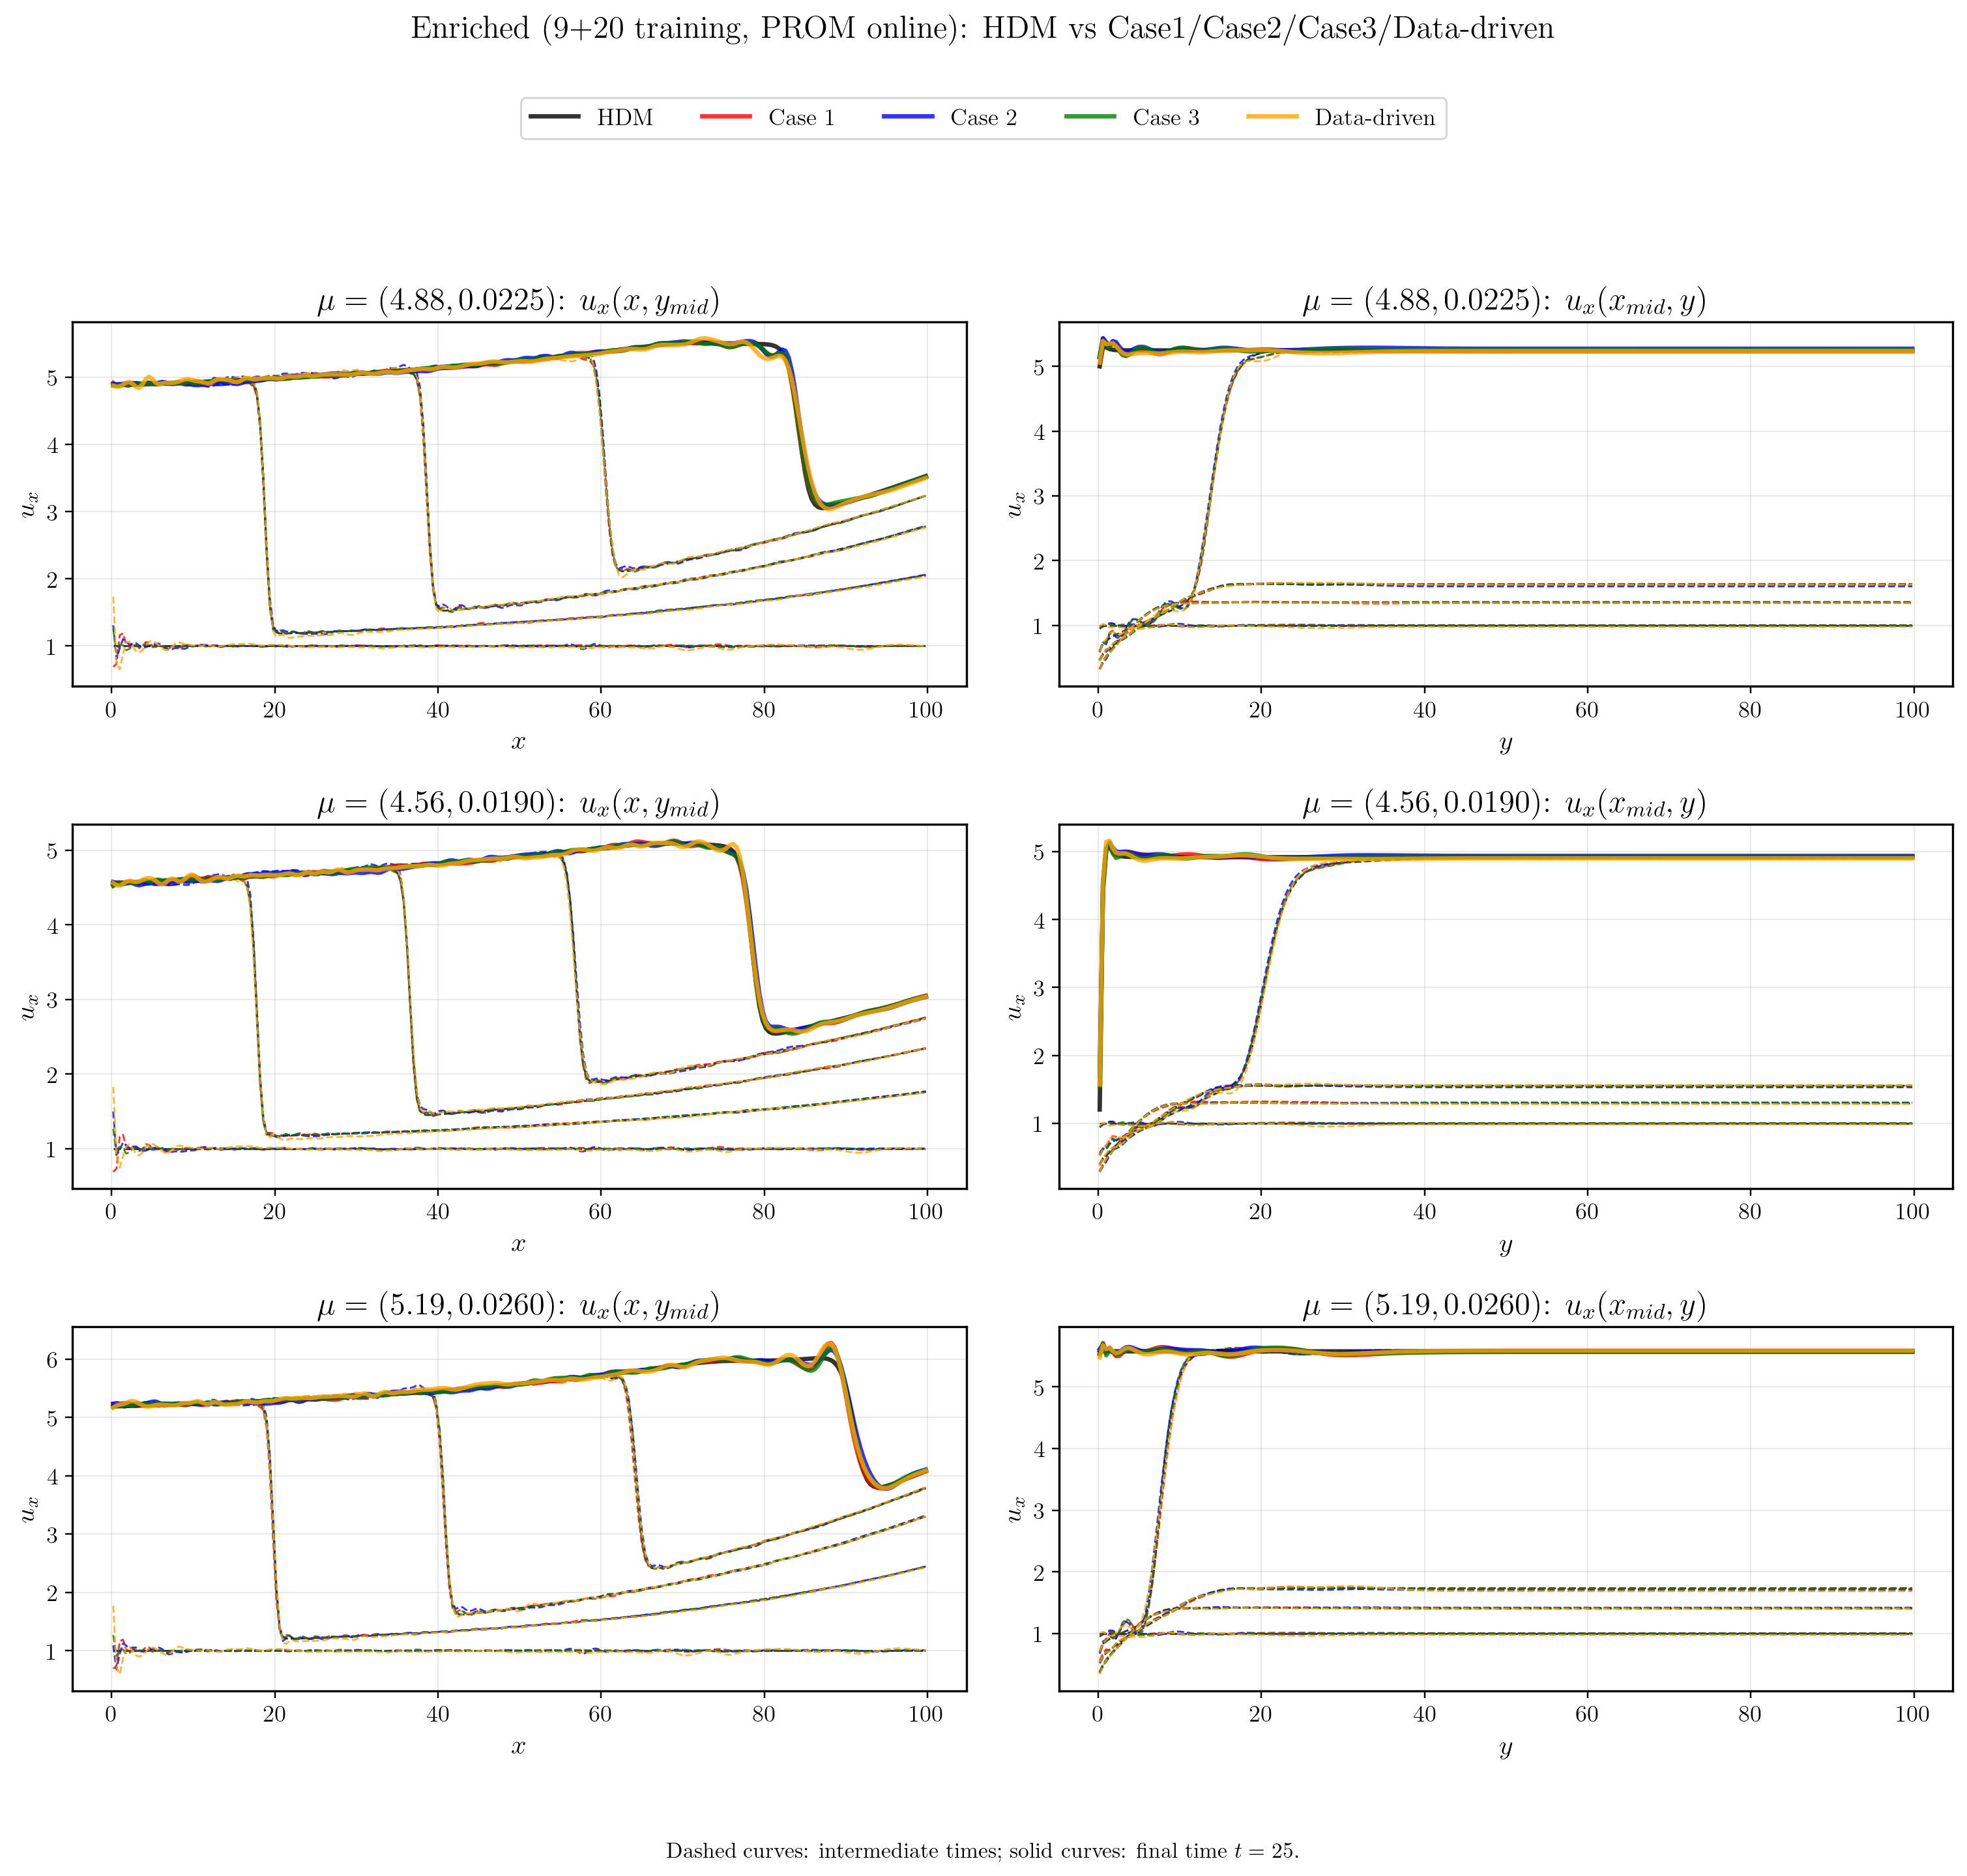
\includegraphics[width=0.98\textwidth]{Figures/enriched_prom_hdm_vs_all_models.png}
\caption{Enriched models, PROM online solve: HDM vs Case~1/2/3 and data-driven at $\bm\mu^{(v)}$, $\bm\mu^{(1)}$, and $\bm\mu^{(2)}$.}
\label{fig:all_models_enriched_prom}
\end{figure}

\appendix
\section{Additional Per-Index Coefficient Error Curves}
\label{app:coeff_curves_extra}

\begin{figure}[H]
\centering
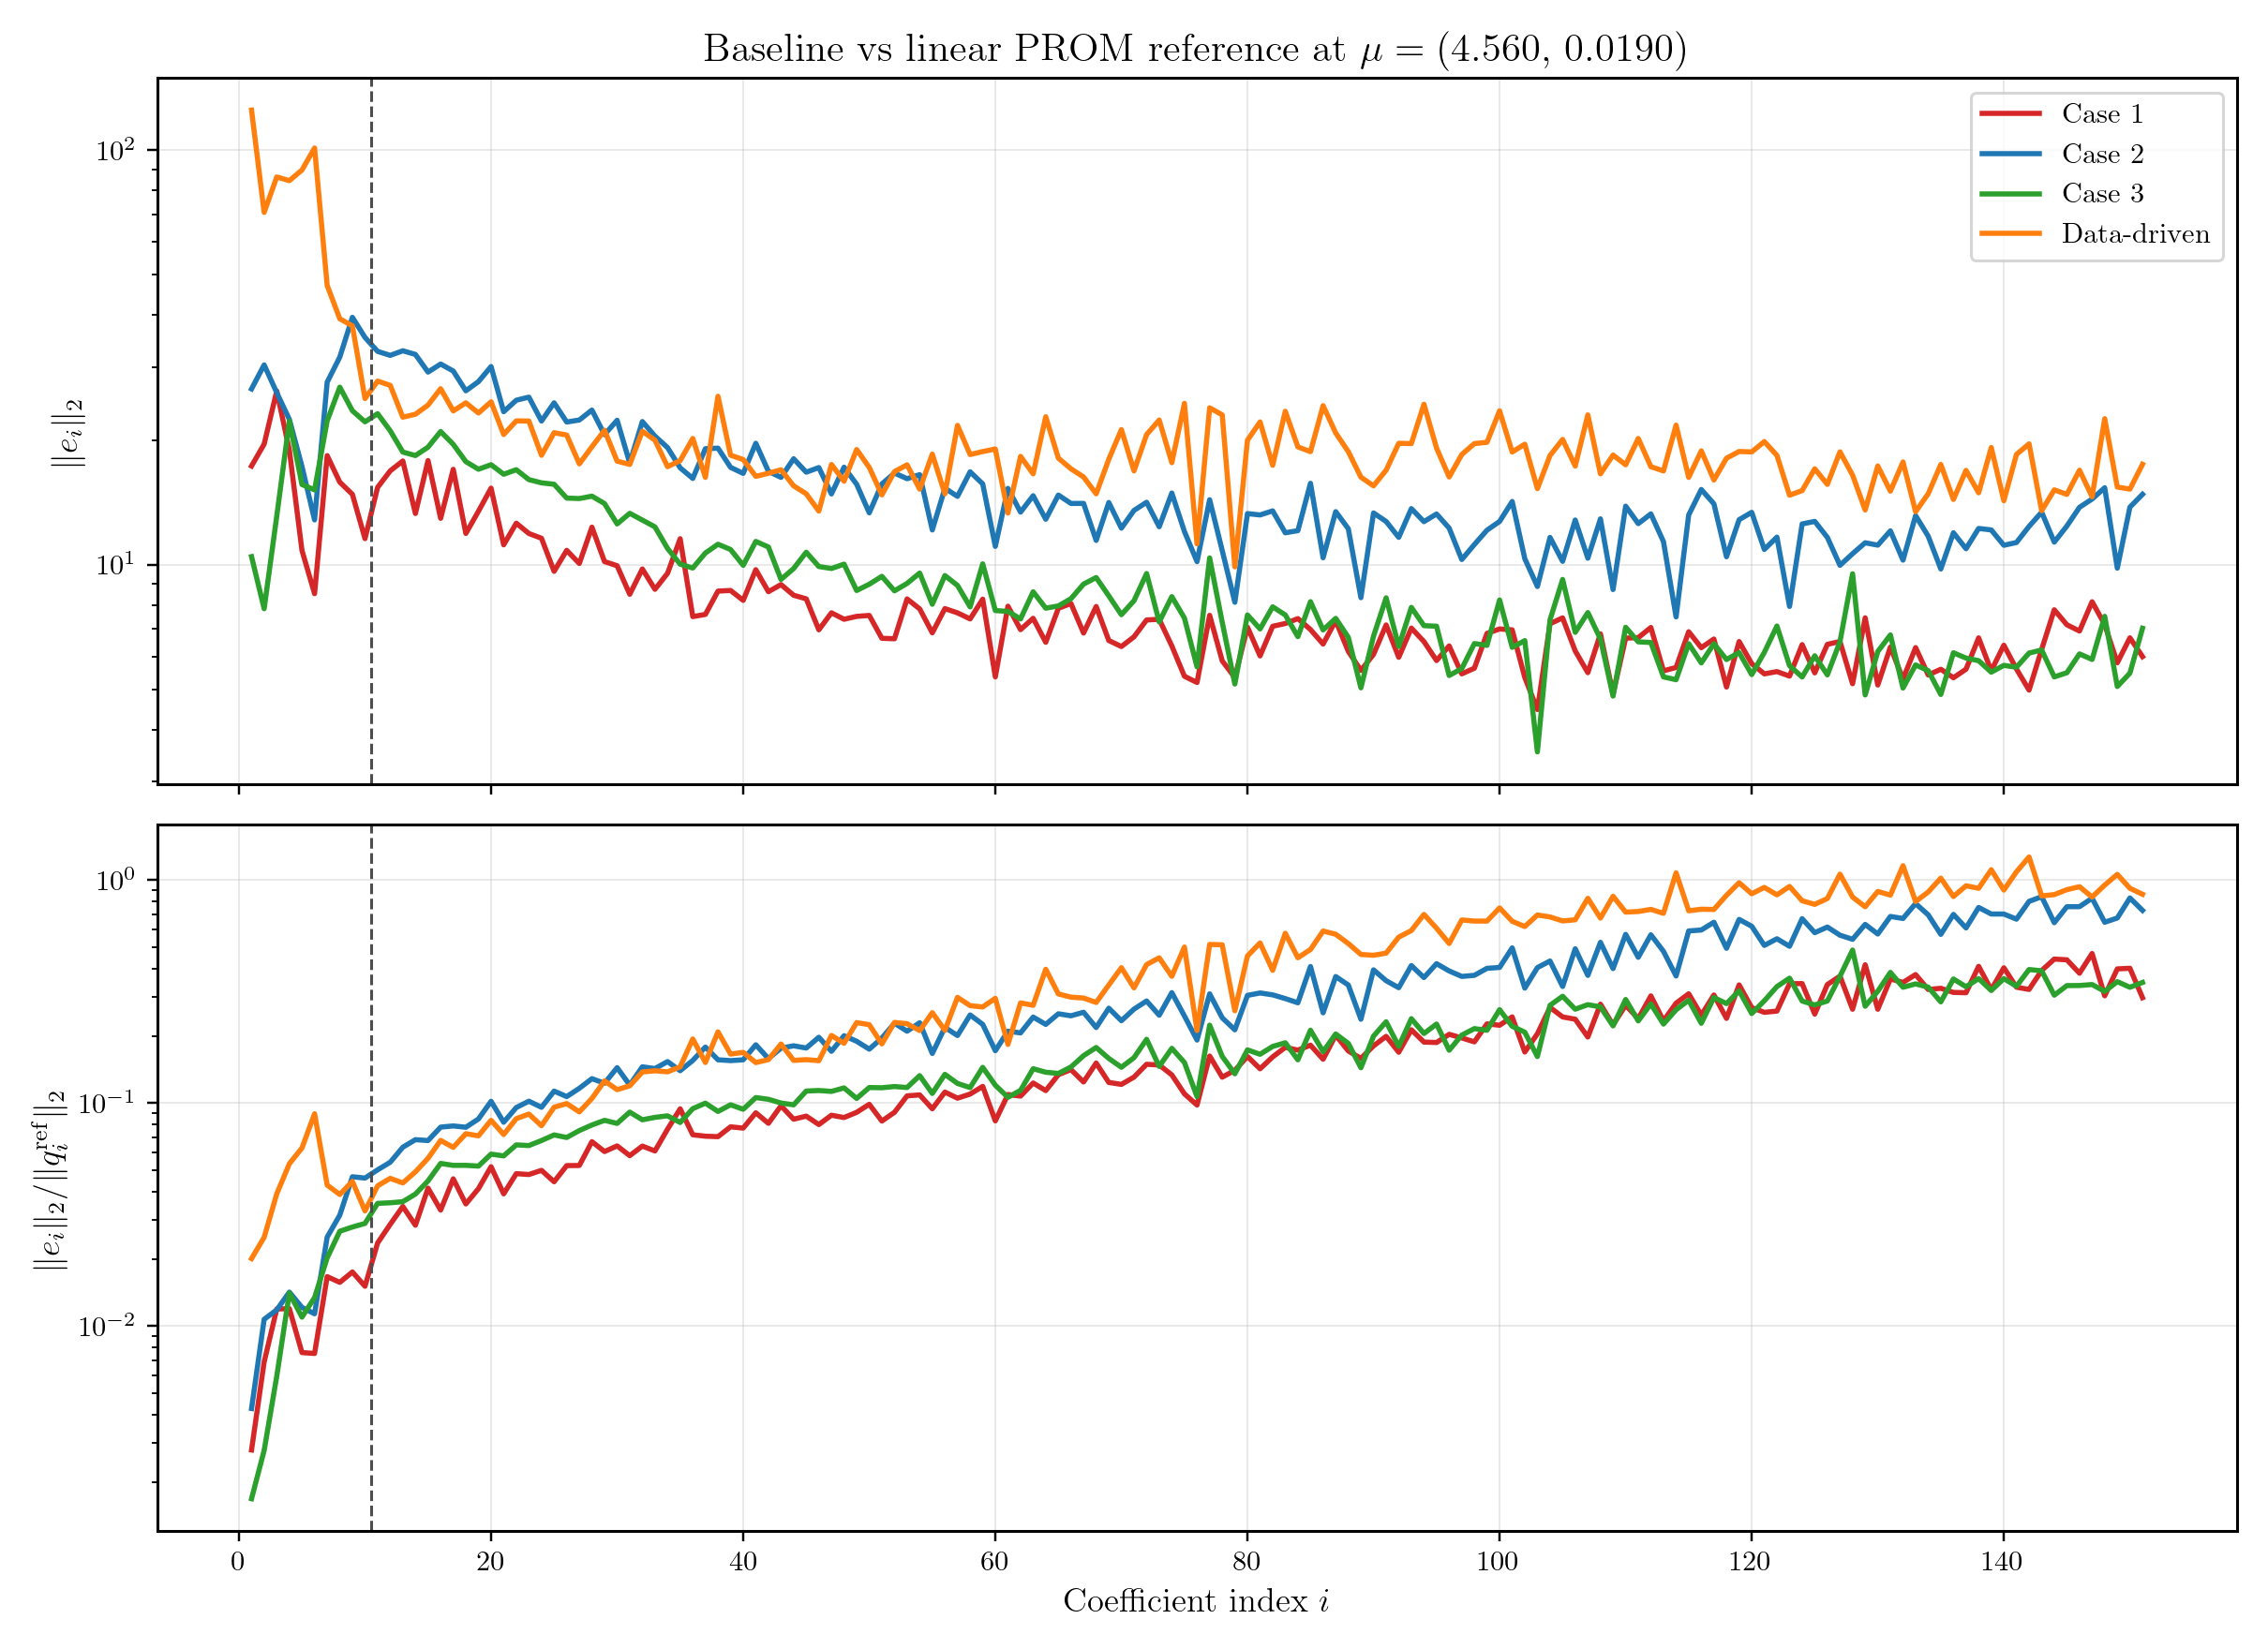
\includegraphics[width=0.94\textwidth]{Figures/coeff_errors/baseline_mu1_4.560_mu2_0.0190_coeff_abs_rel_vs_index.png}
\caption{Baseline stage: per-index absolute and relative coefficient errors at $\bm\mu^{(1)}=(4.56,0.019)$.}
\label{fig:coeff_abs_rel_baseline_mu1}
\end{figure}

\begin{figure}[H]
\centering
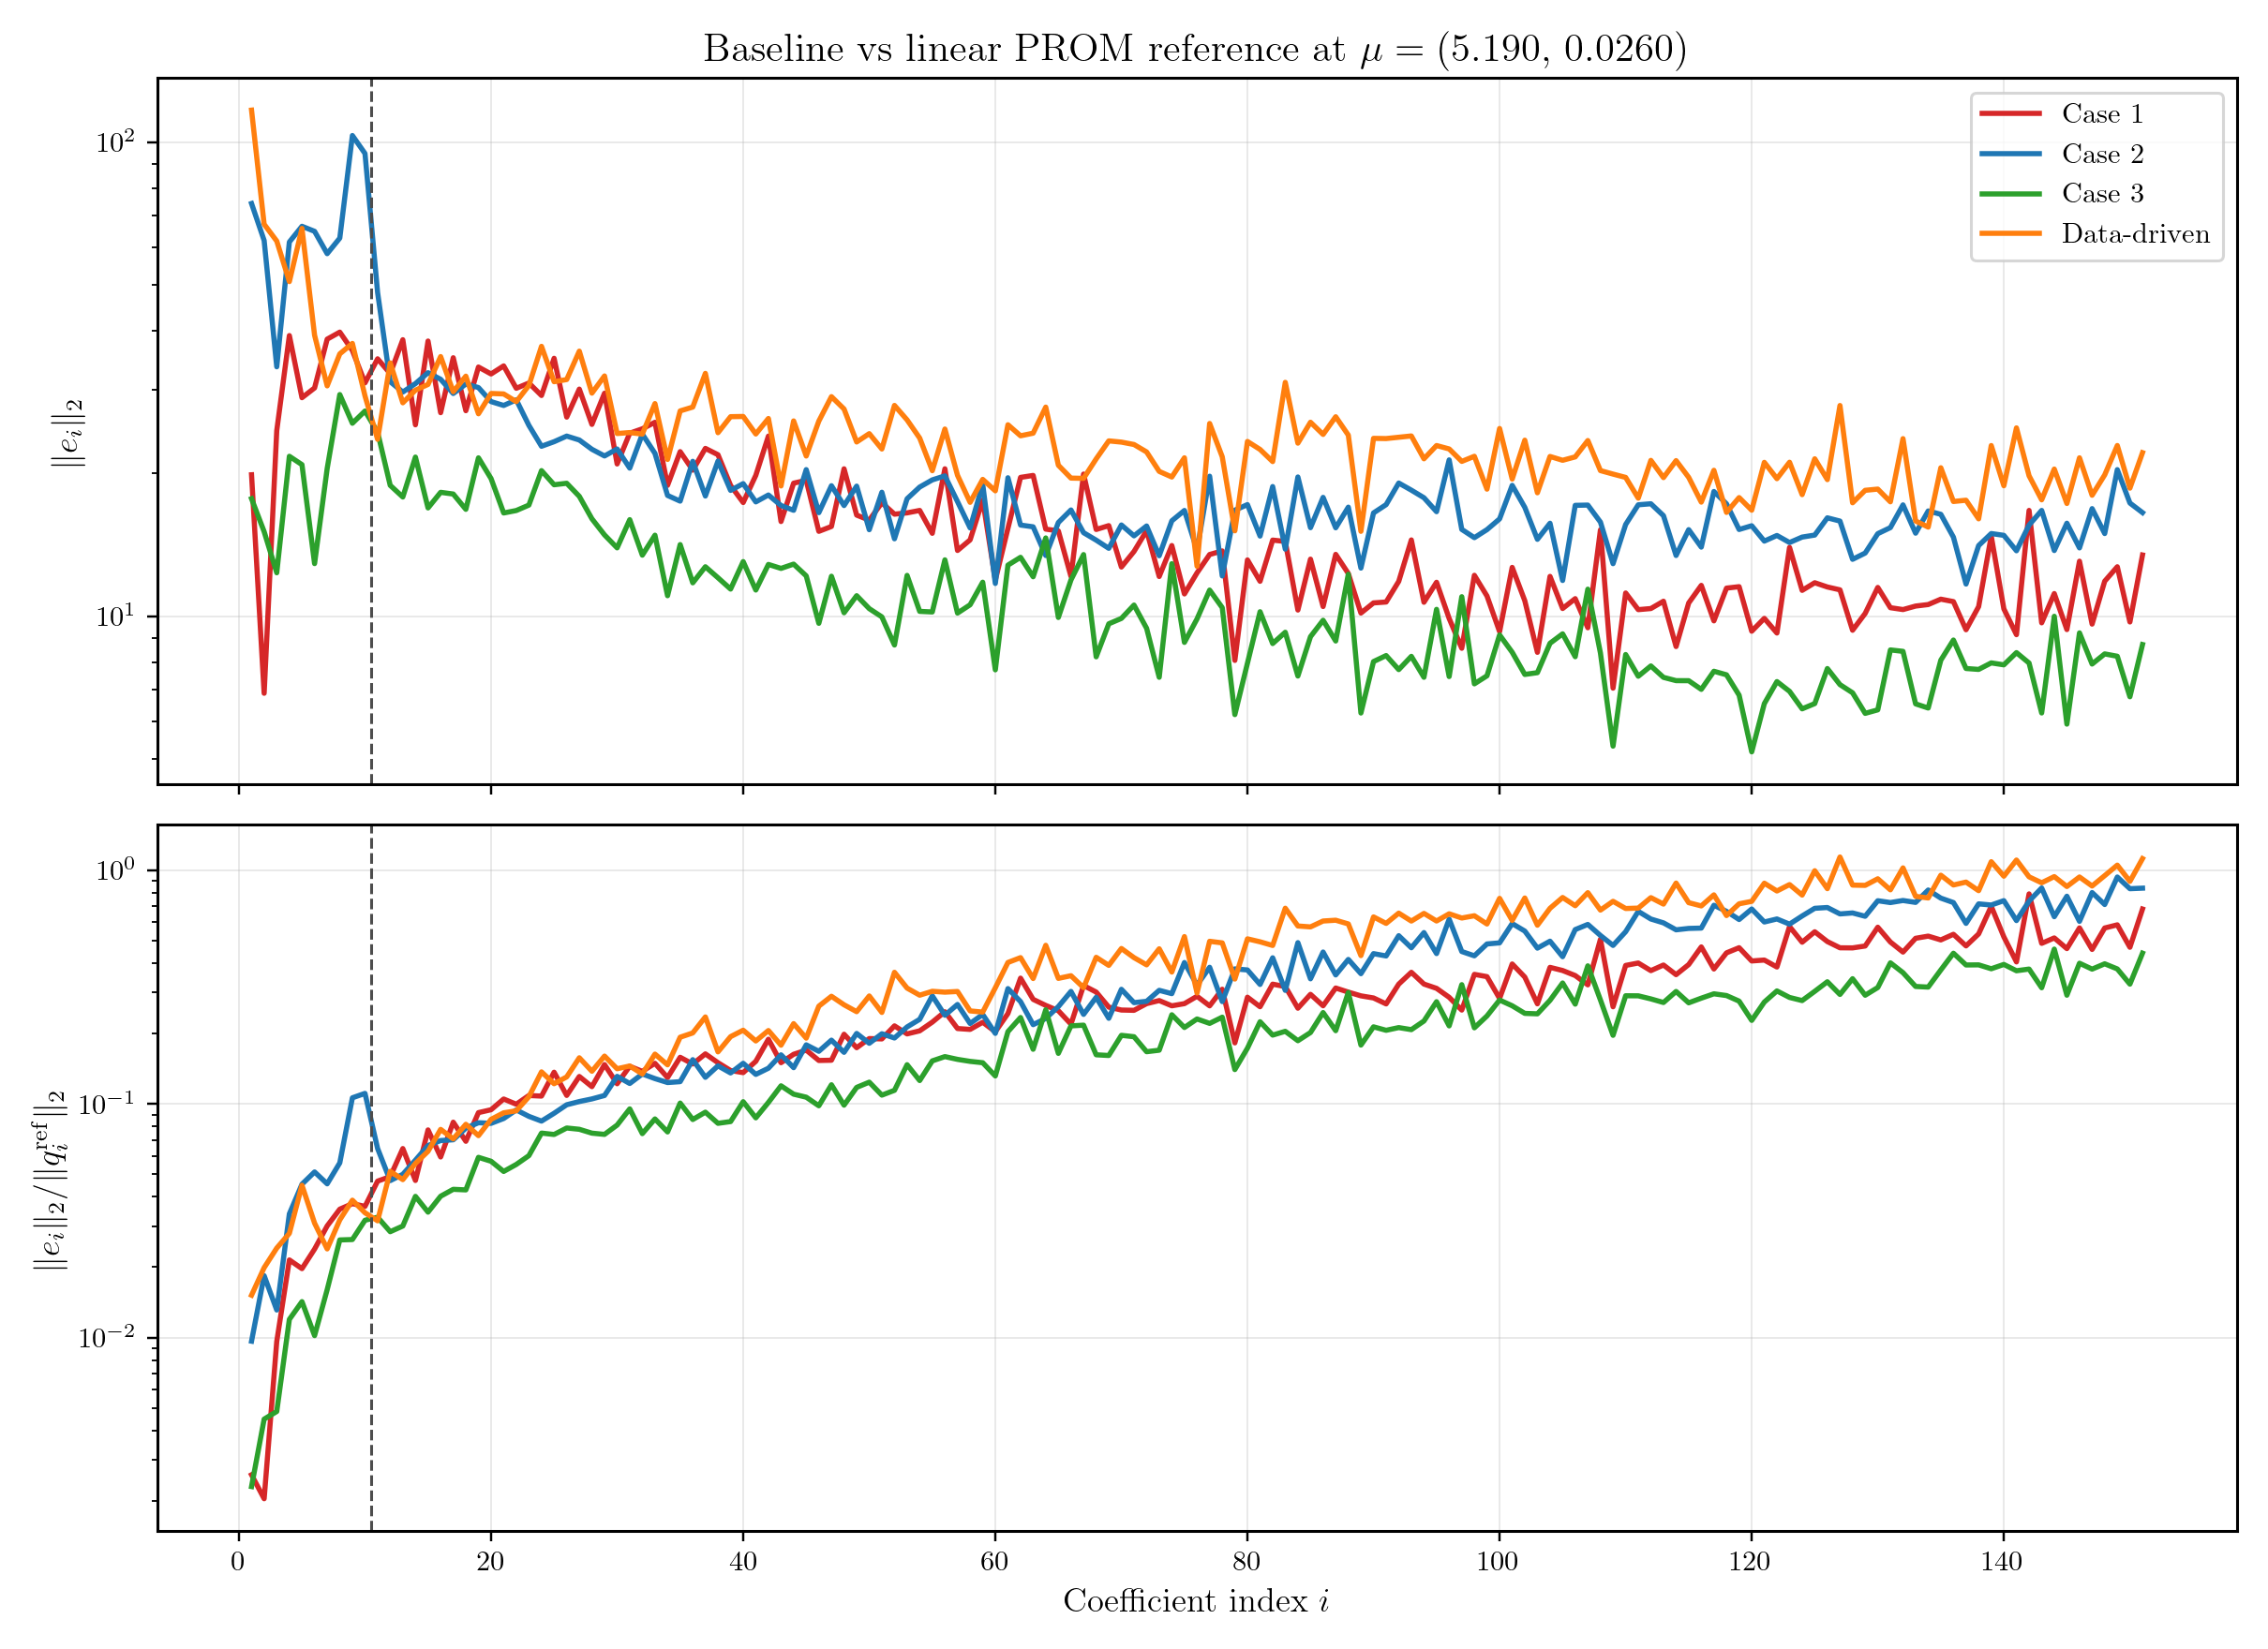
\includegraphics[width=0.94\textwidth]{Figures/coeff_errors/baseline_mu1_5.190_mu2_0.0260_coeff_abs_rel_vs_index.png}
\caption{Baseline stage: per-index absolute and relative coefficient errors at $\bm\mu^{(2)}=(5.19,0.026)$.}
\label{fig:coeff_abs_rel_baseline_mu2}
\end{figure}

\begin{figure}[H]
\centering
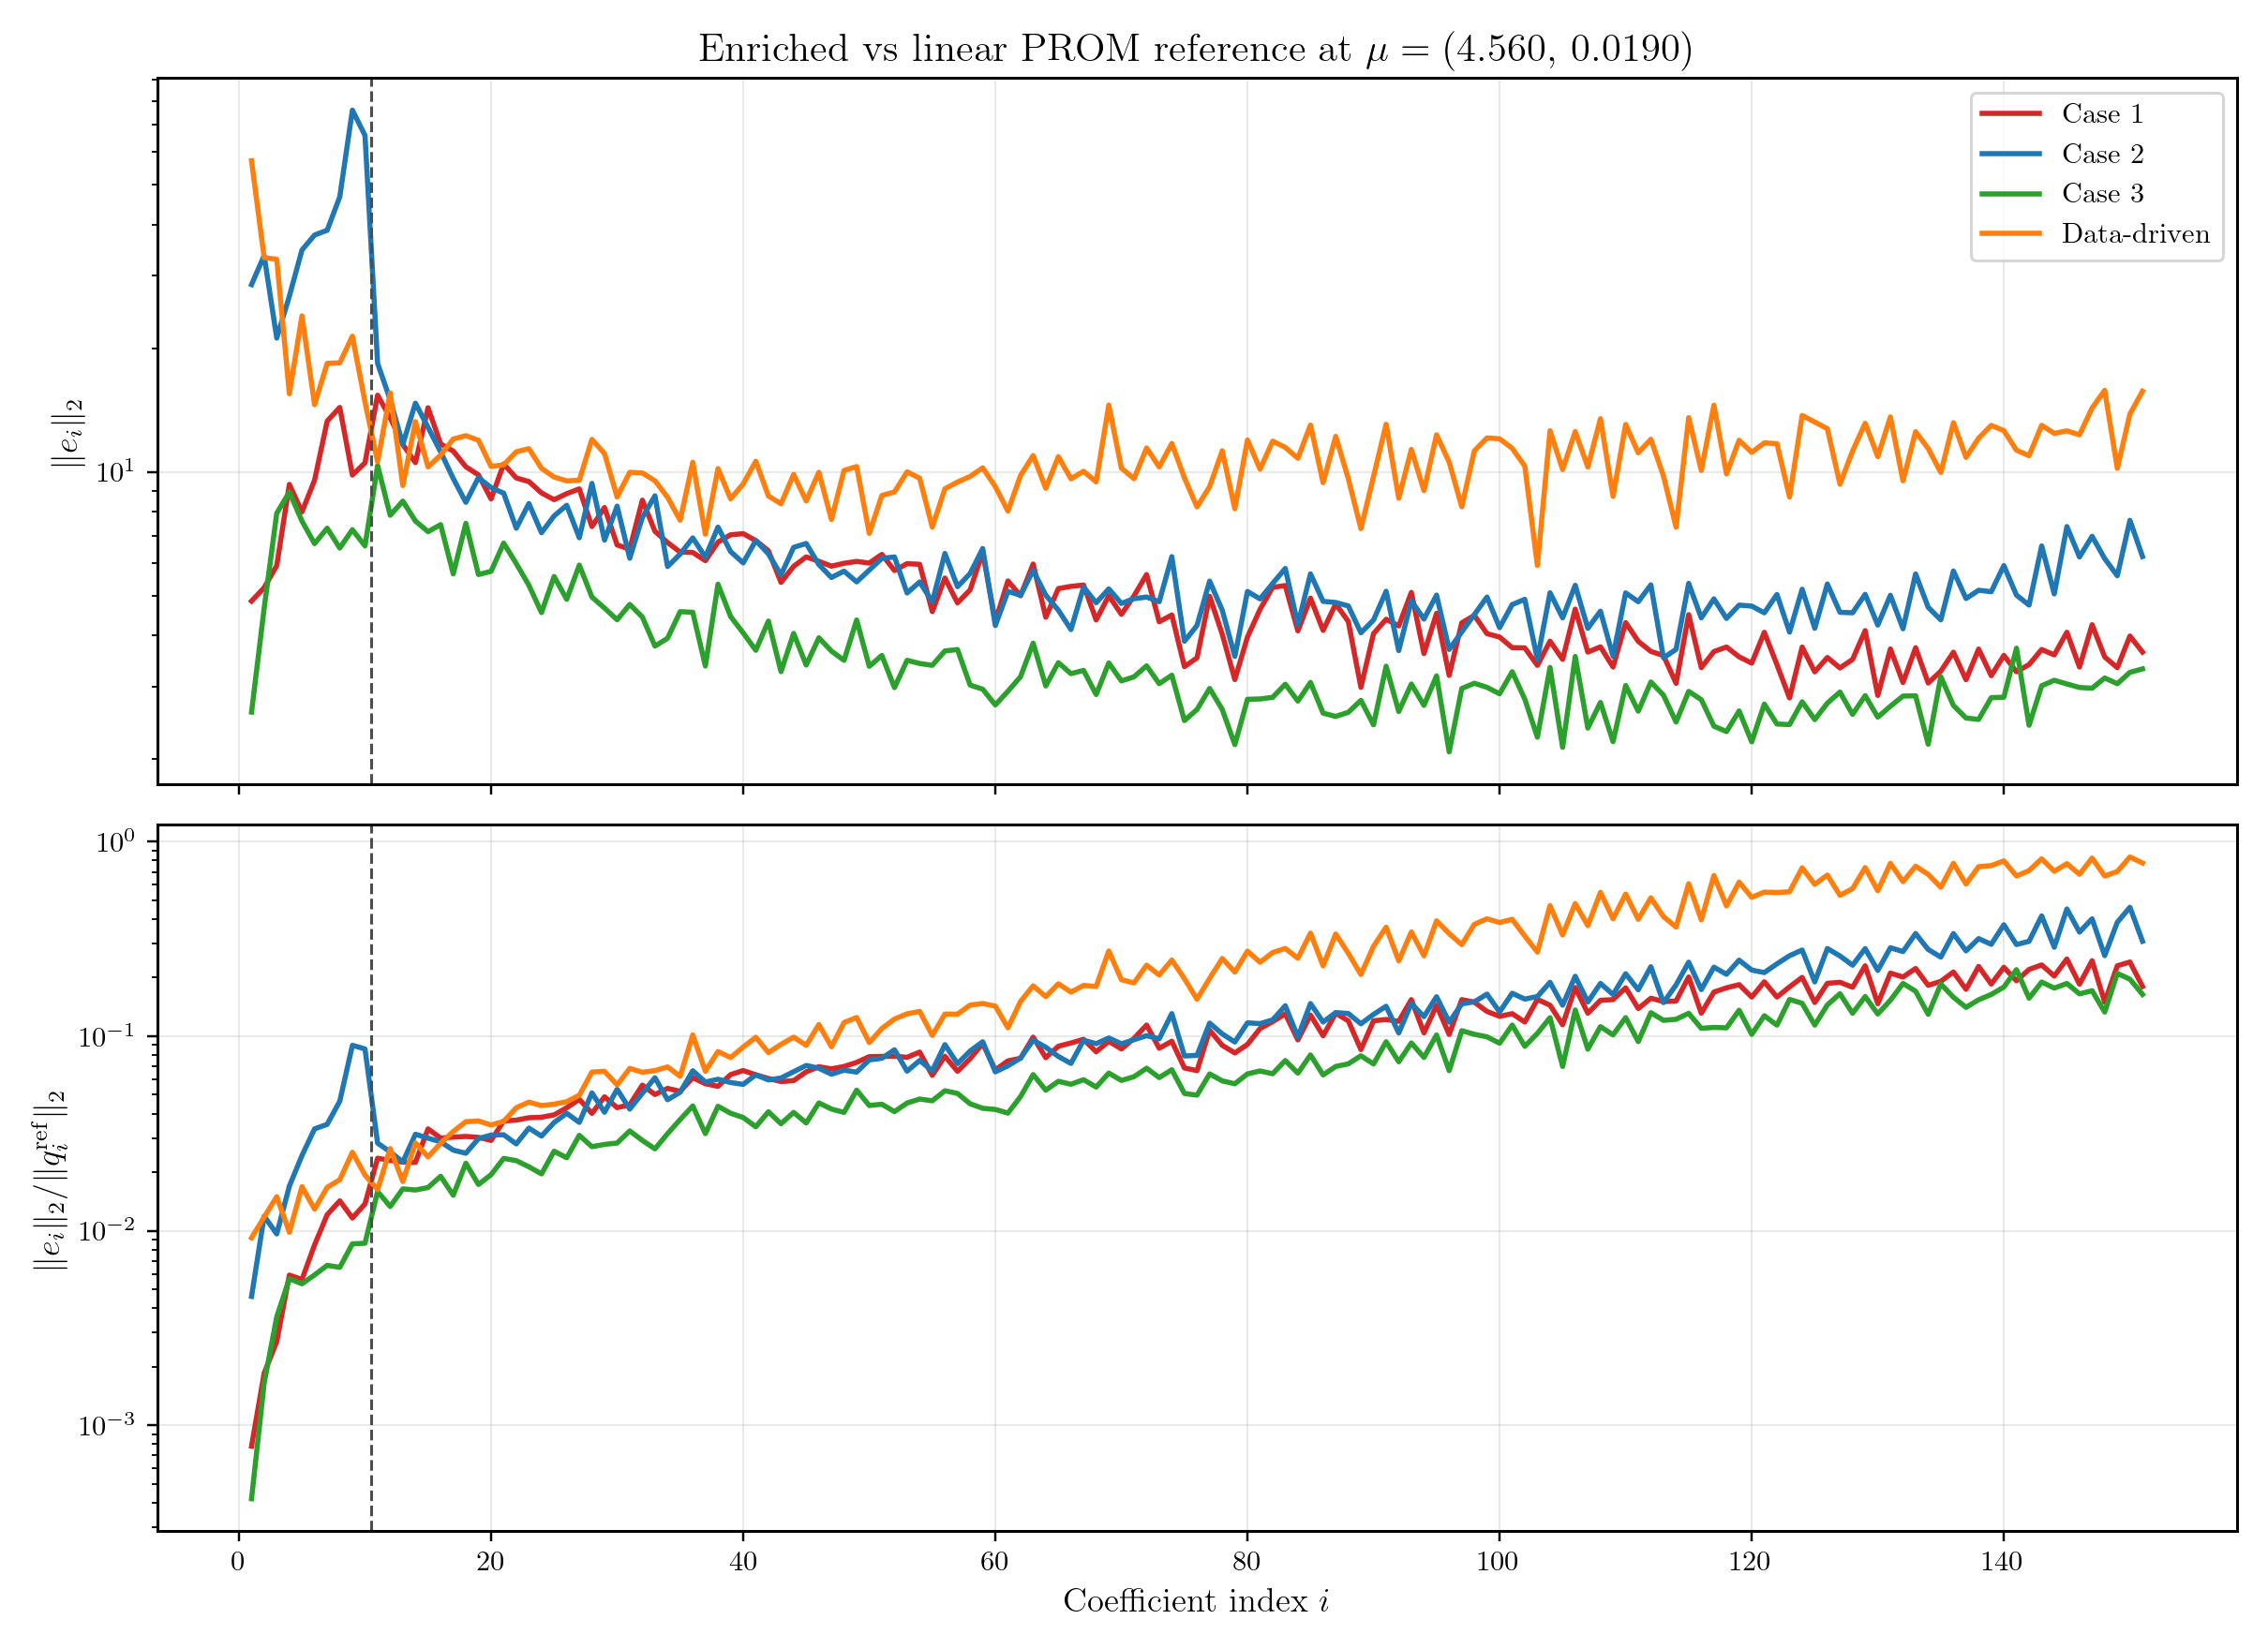
\includegraphics[width=0.94\textwidth]{Figures/coeff_errors/enriched_mu1_4.560_mu2_0.0190_coeff_abs_rel_vs_index.png}
\caption{Enriched stage: per-index absolute and relative coefficient errors at $\bm\mu^{(1)}=(4.56,0.019)$.}
\label{fig:coeff_abs_rel_enriched_mu1}
\end{figure}

\begin{figure}[H]
\centering
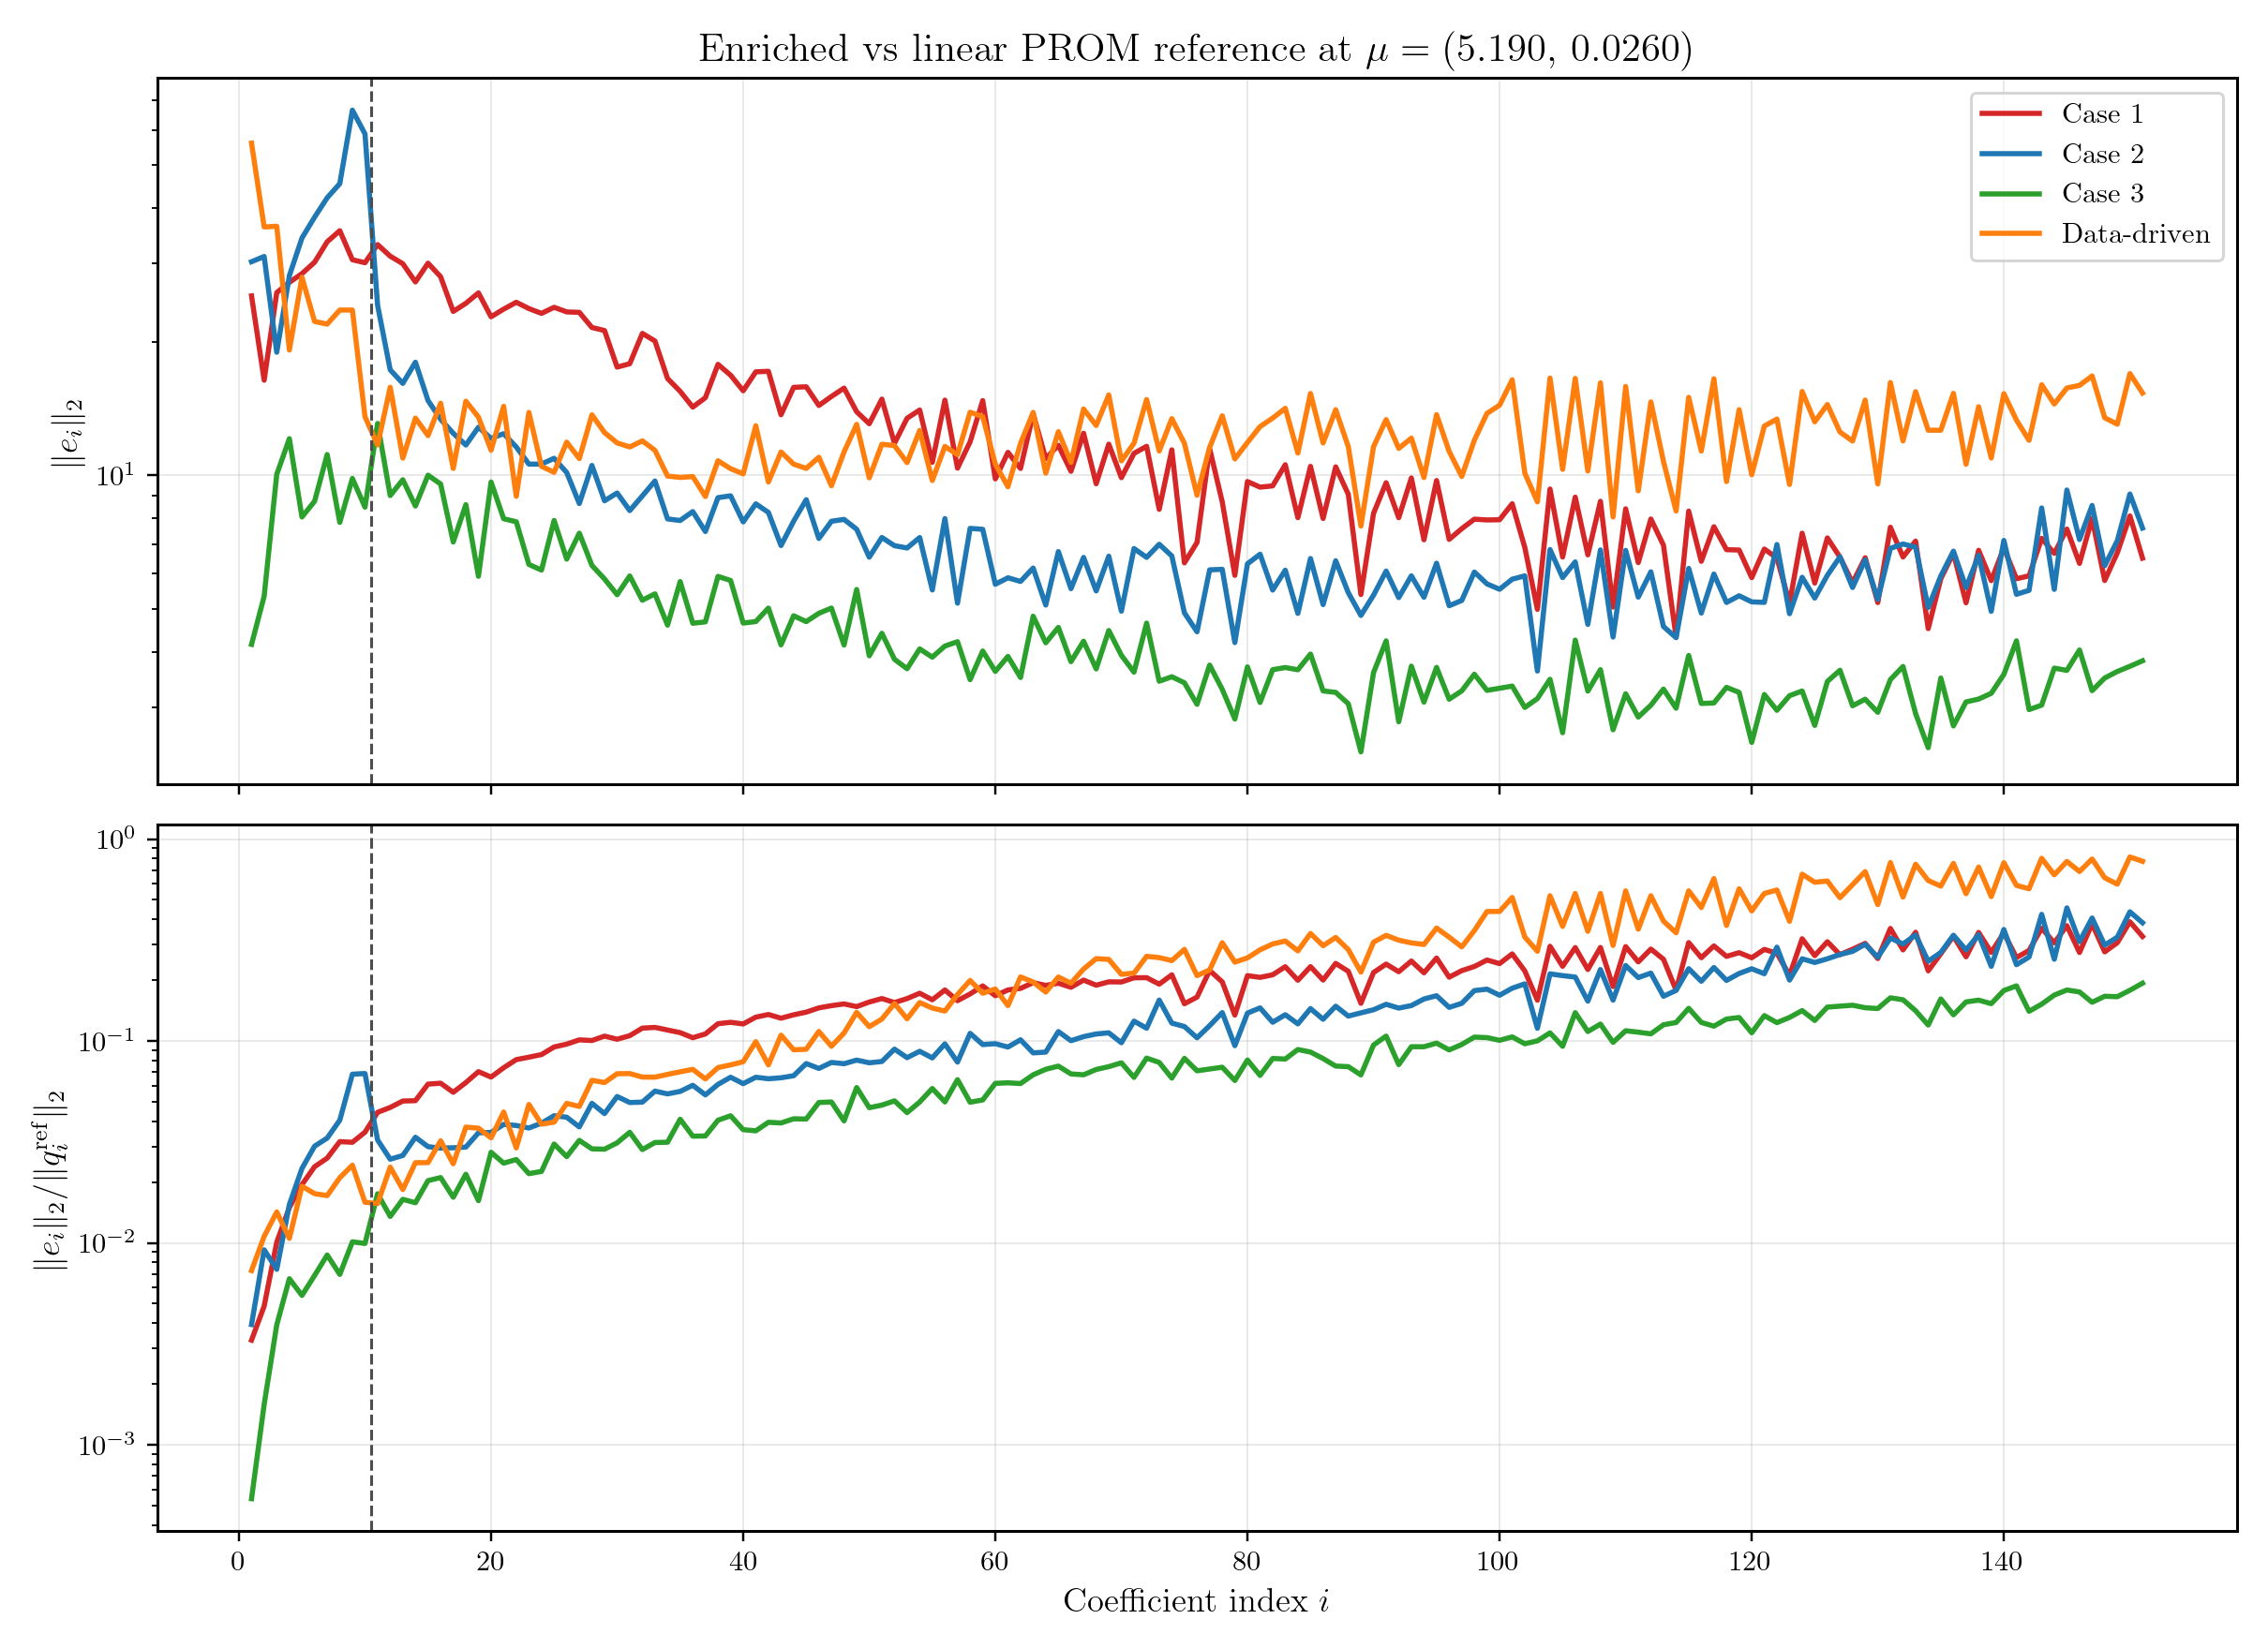
\includegraphics[width=0.94\textwidth]{Figures/coeff_errors/enriched_mu1_5.190_mu2_0.0260_coeff_abs_rel_vs_index.png}
\caption{Enriched stage: per-index absolute and relative coefficient errors at $\bm\mu^{(2)}=(5.19,0.026)$.}
\label{fig:coeff_abs_rel_enriched_mu2}
\end{figure}

\section{Time-Resolved Coefficient Error Heatmaps}
\label{app:coeff_heatmaps}

To visualize error propagation in time, we report coefficient-index vs time heatmaps at $\bm\mu^{(v)}$, $\bm\mu^{(1)}$, and $\bm\mu^{(2)}$, with linear $n_{\mathrm{tot}}$-PROM coefficients as reference.

\begin{figure}[H]
\centering
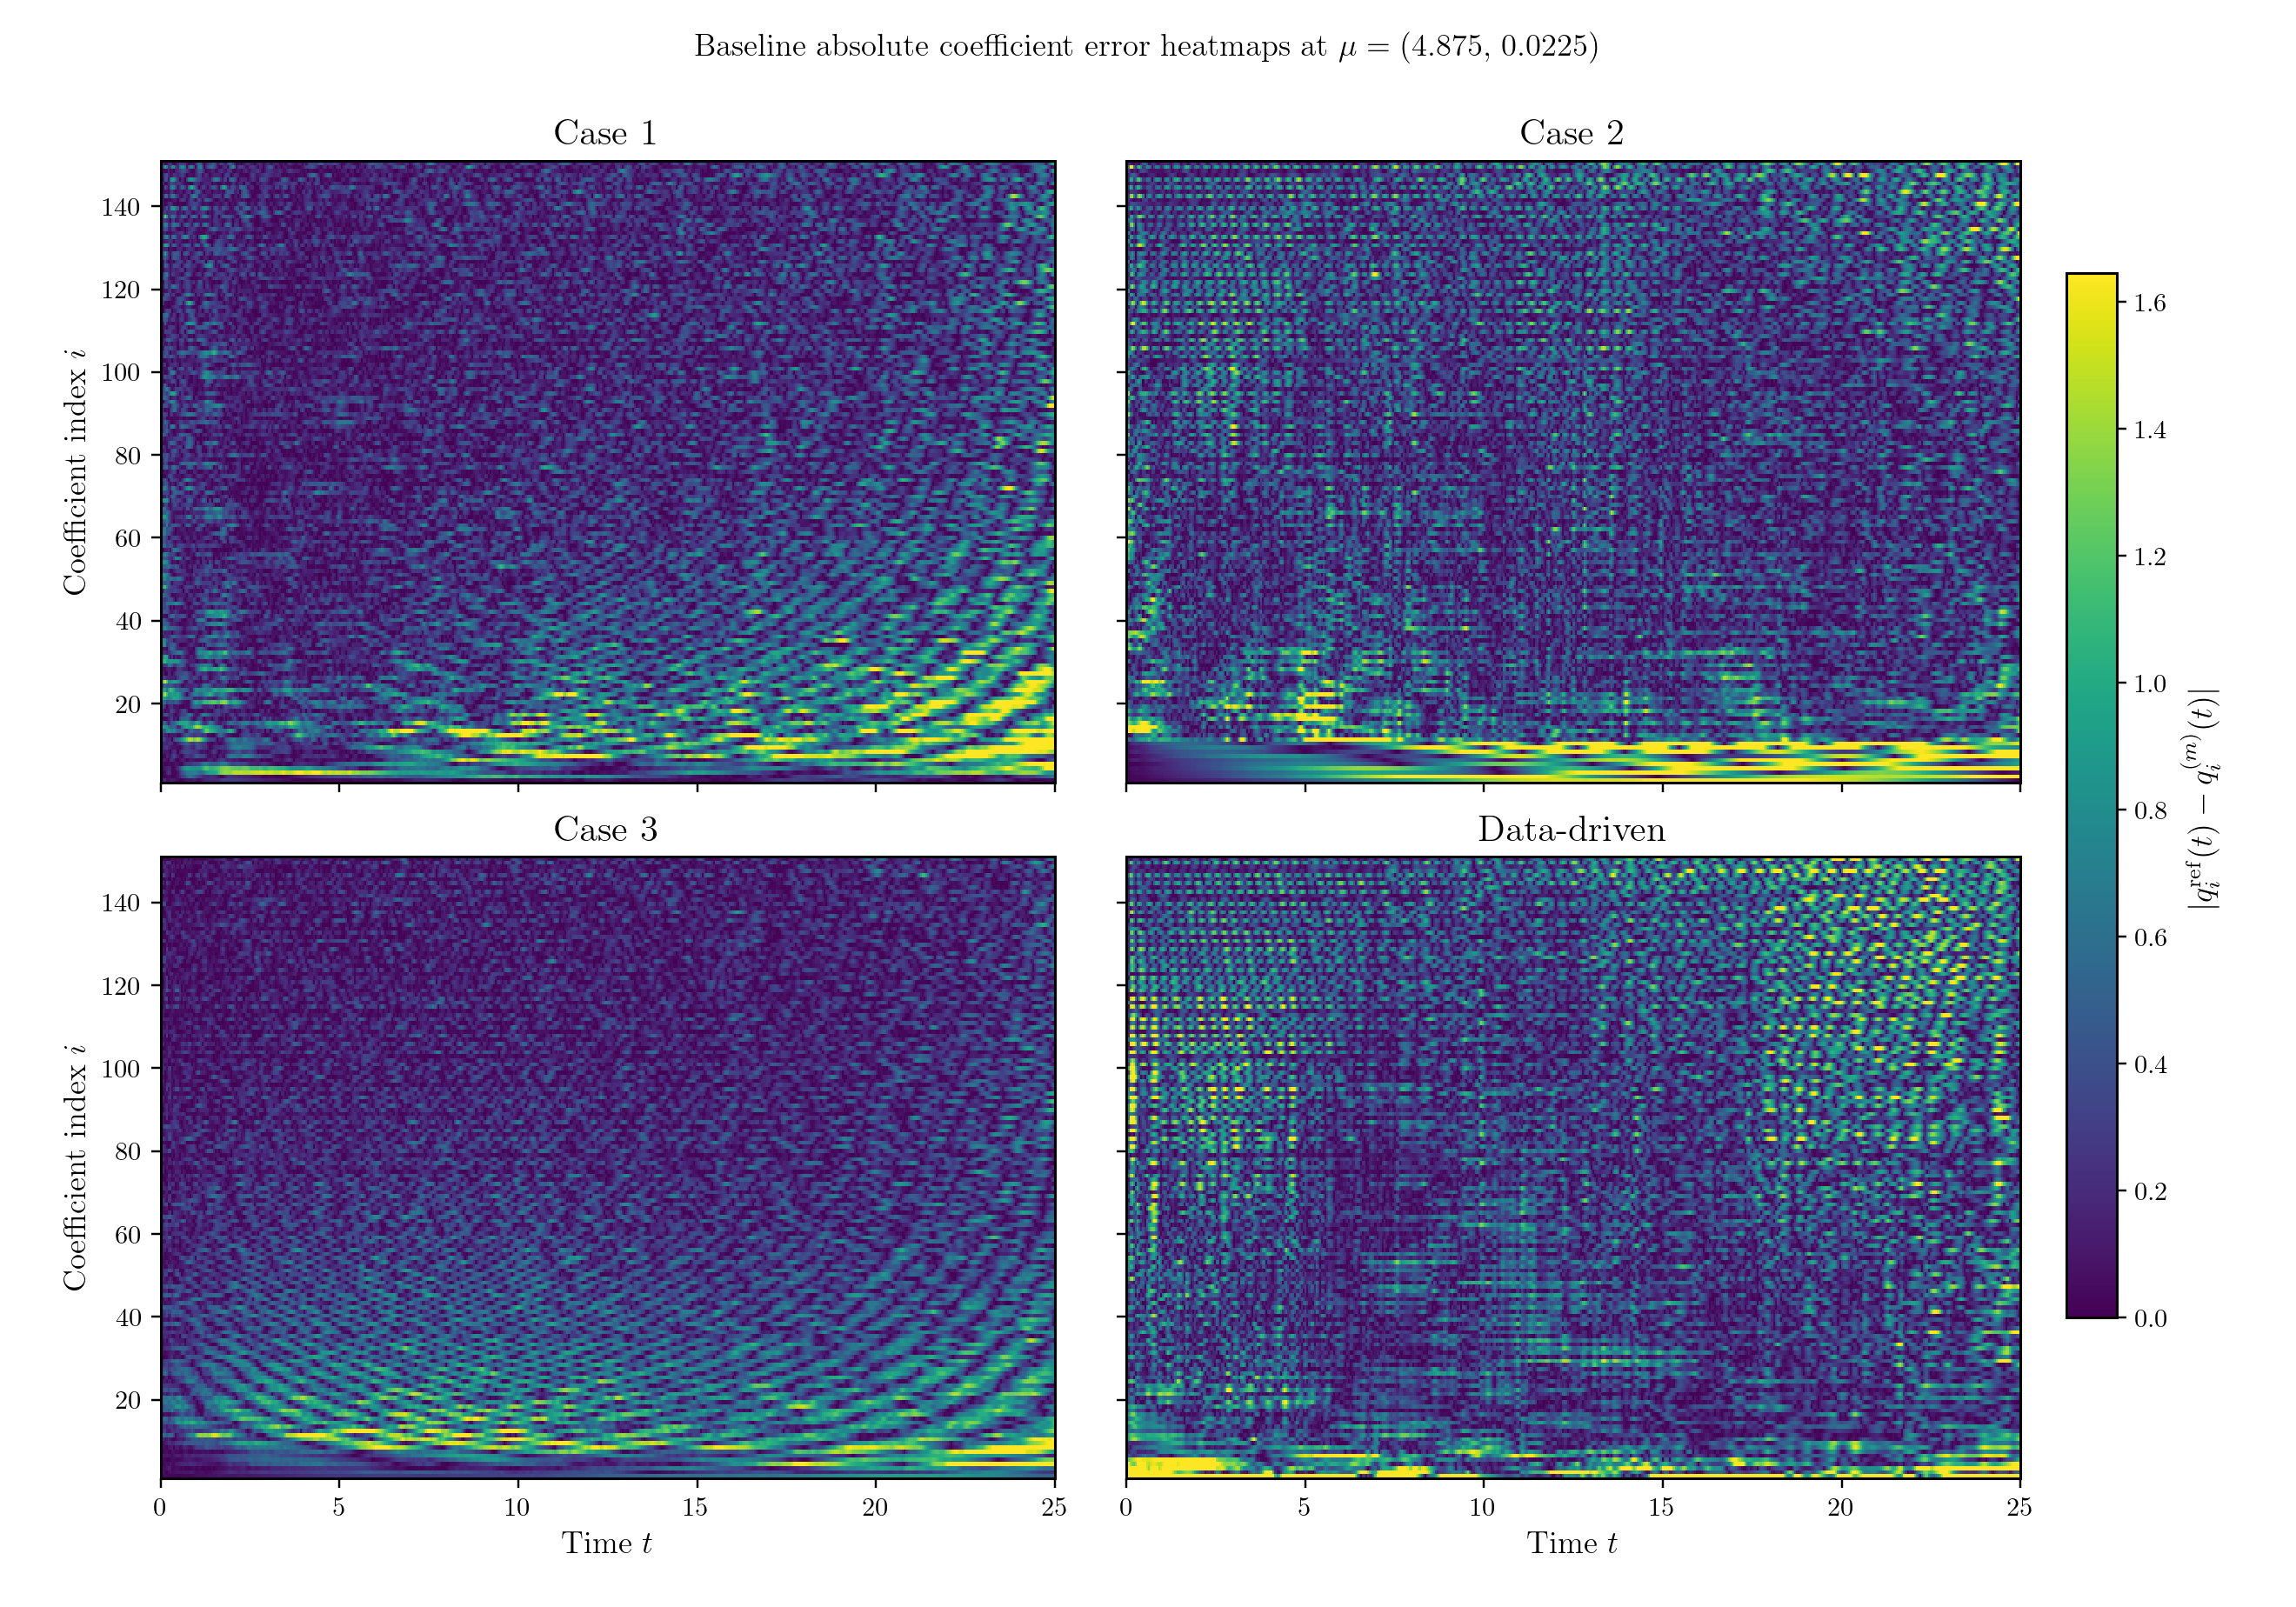
\includegraphics[width=0.98\textwidth]{Figures/coeff_errors/baseline_mu1_4.875_mu2_0.0225_coeff_abs_heatmap_grid.png}
\caption{Baseline stage: absolute coefficient error heatmaps $\left|q_i^{\mathrm{ref}}(t)-q_i^{(m)}(t)\right|$ for Case~1, Case~2, Case~3, and data-driven models.}
\label{fig:hm_baseline_abs_verif}
\end{figure}

\begin{figure}[H]
\centering
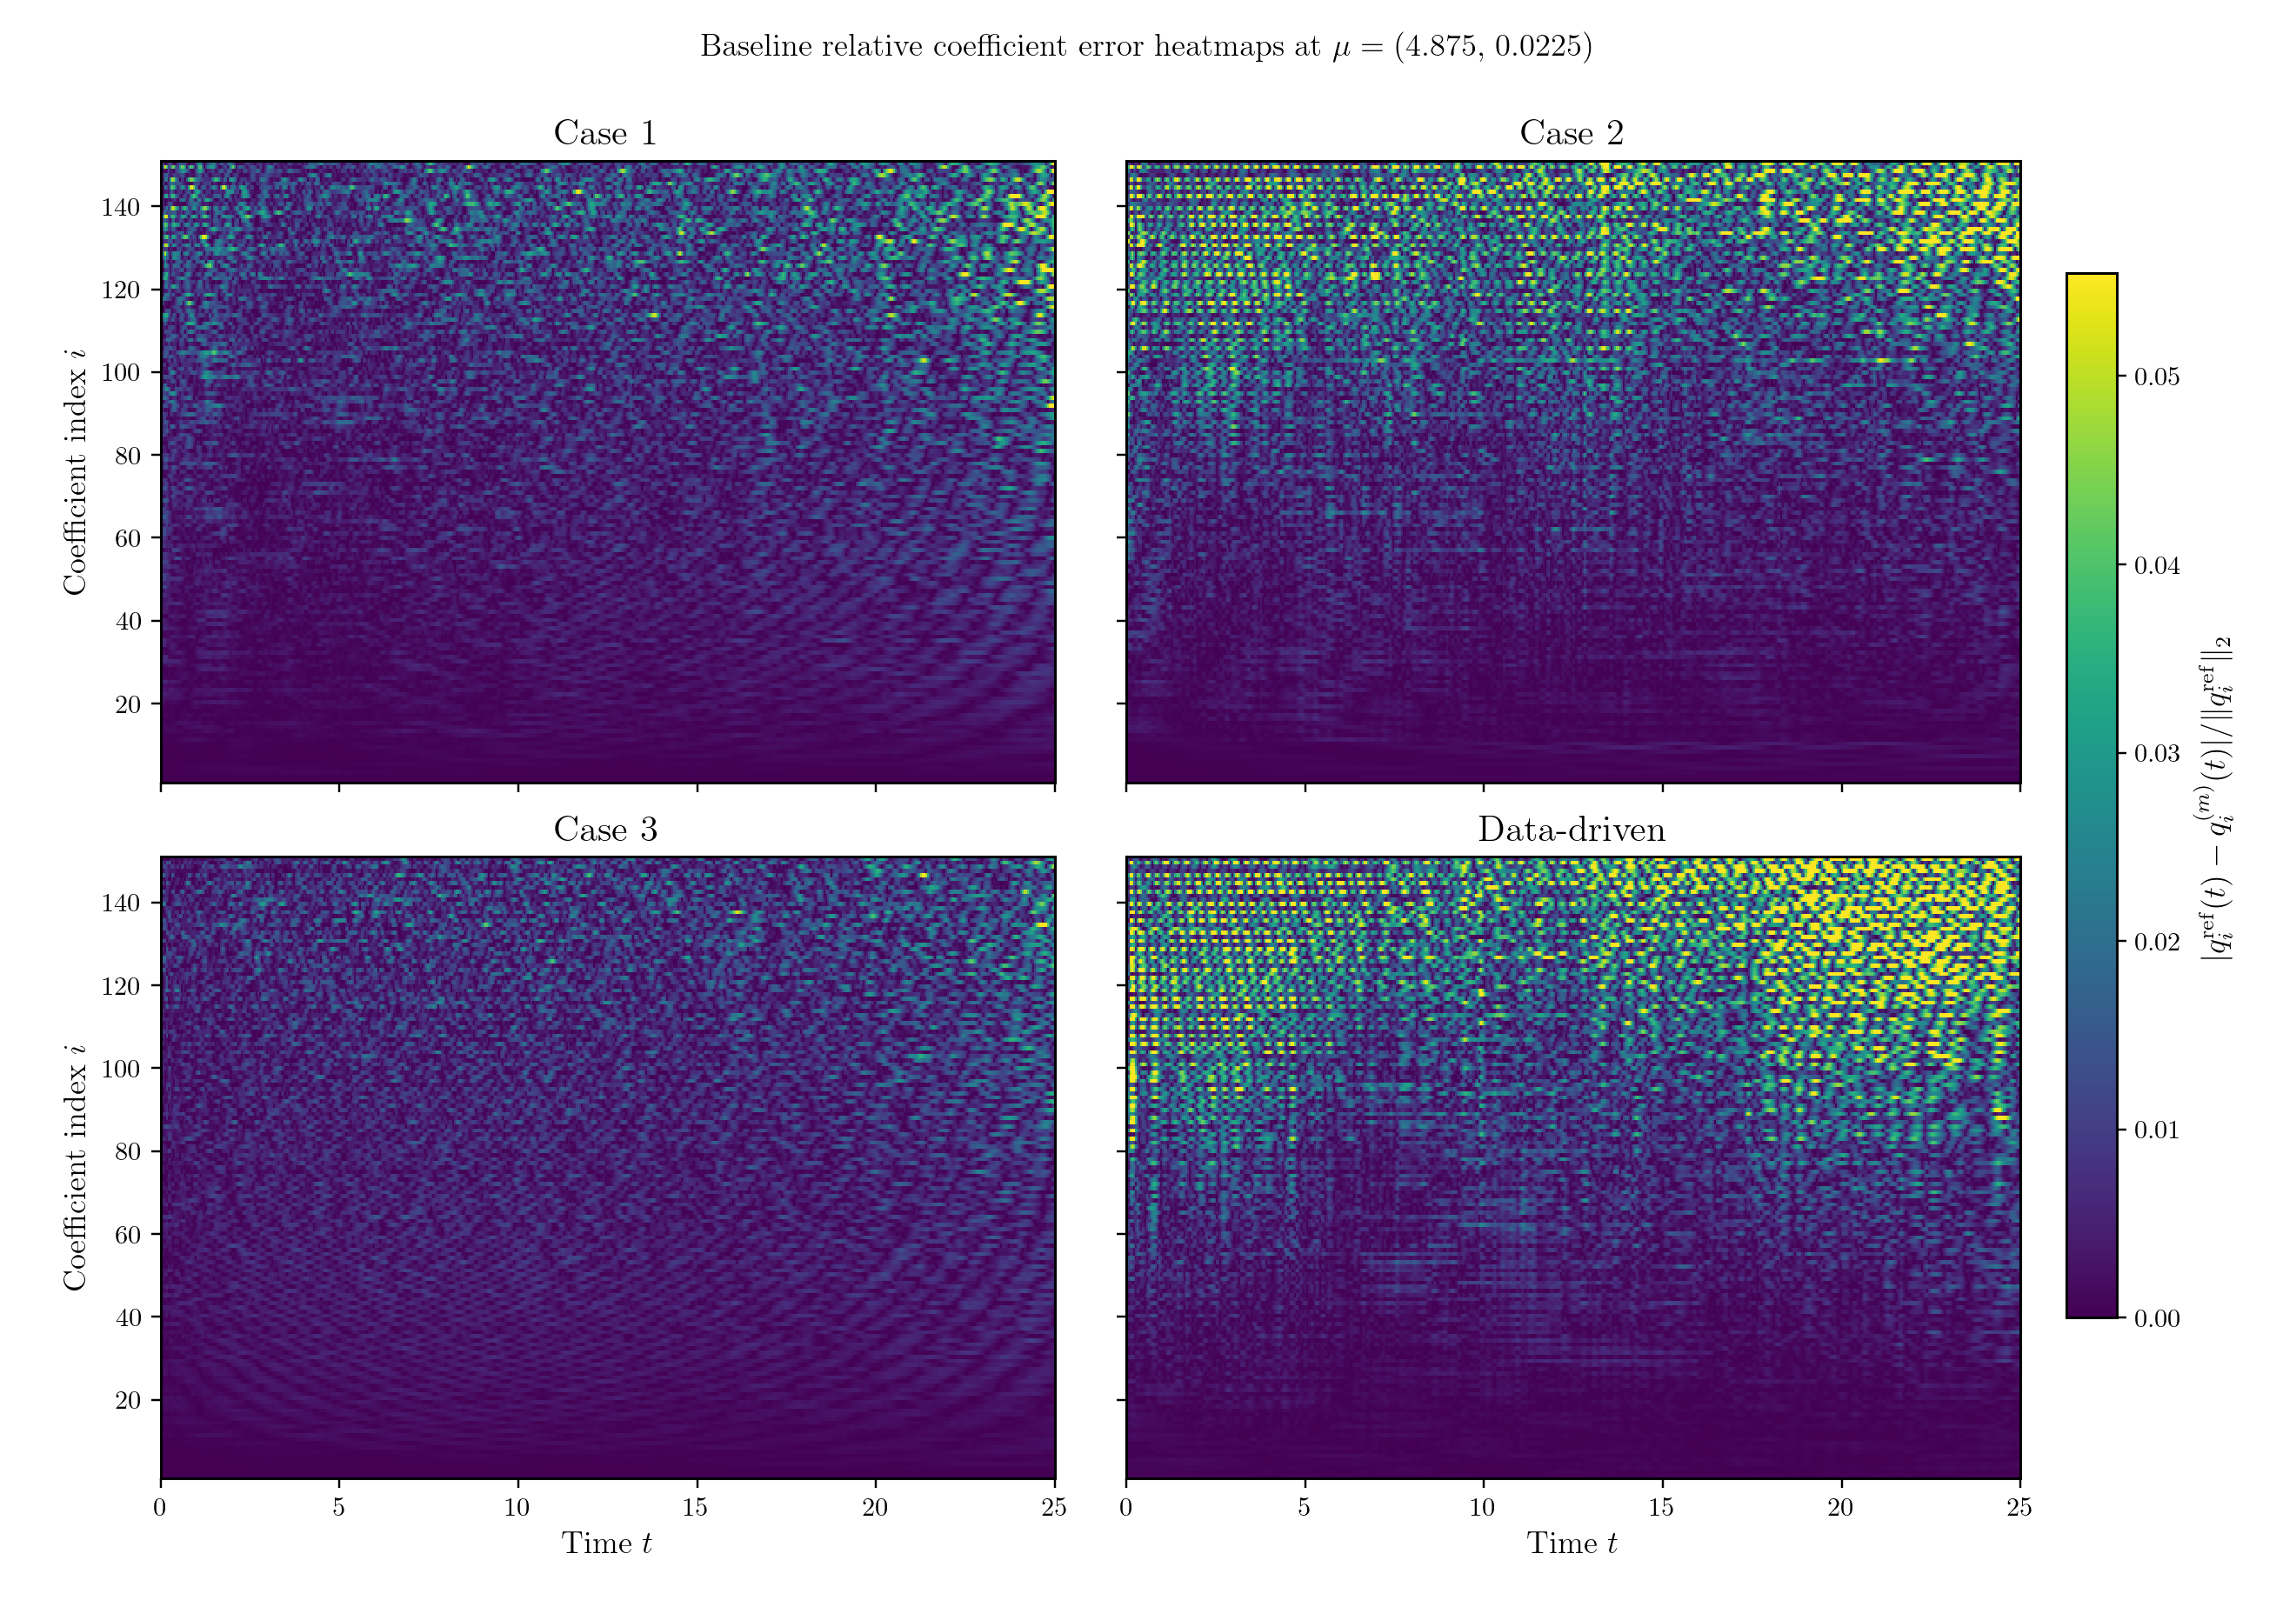
\includegraphics[width=0.98\textwidth]{Figures/coeff_errors/baseline_mu1_4.875_mu2_0.0225_coeff_rel_heatmap_grid.png}
\caption{Baseline stage: relative coefficient error heatmaps using normalization by $\|q_i^{\mathrm{ref}}\|_2$.}
\label{fig:hm_baseline_rel_verif}
\end{figure}

\begin{figure}[H]
\centering
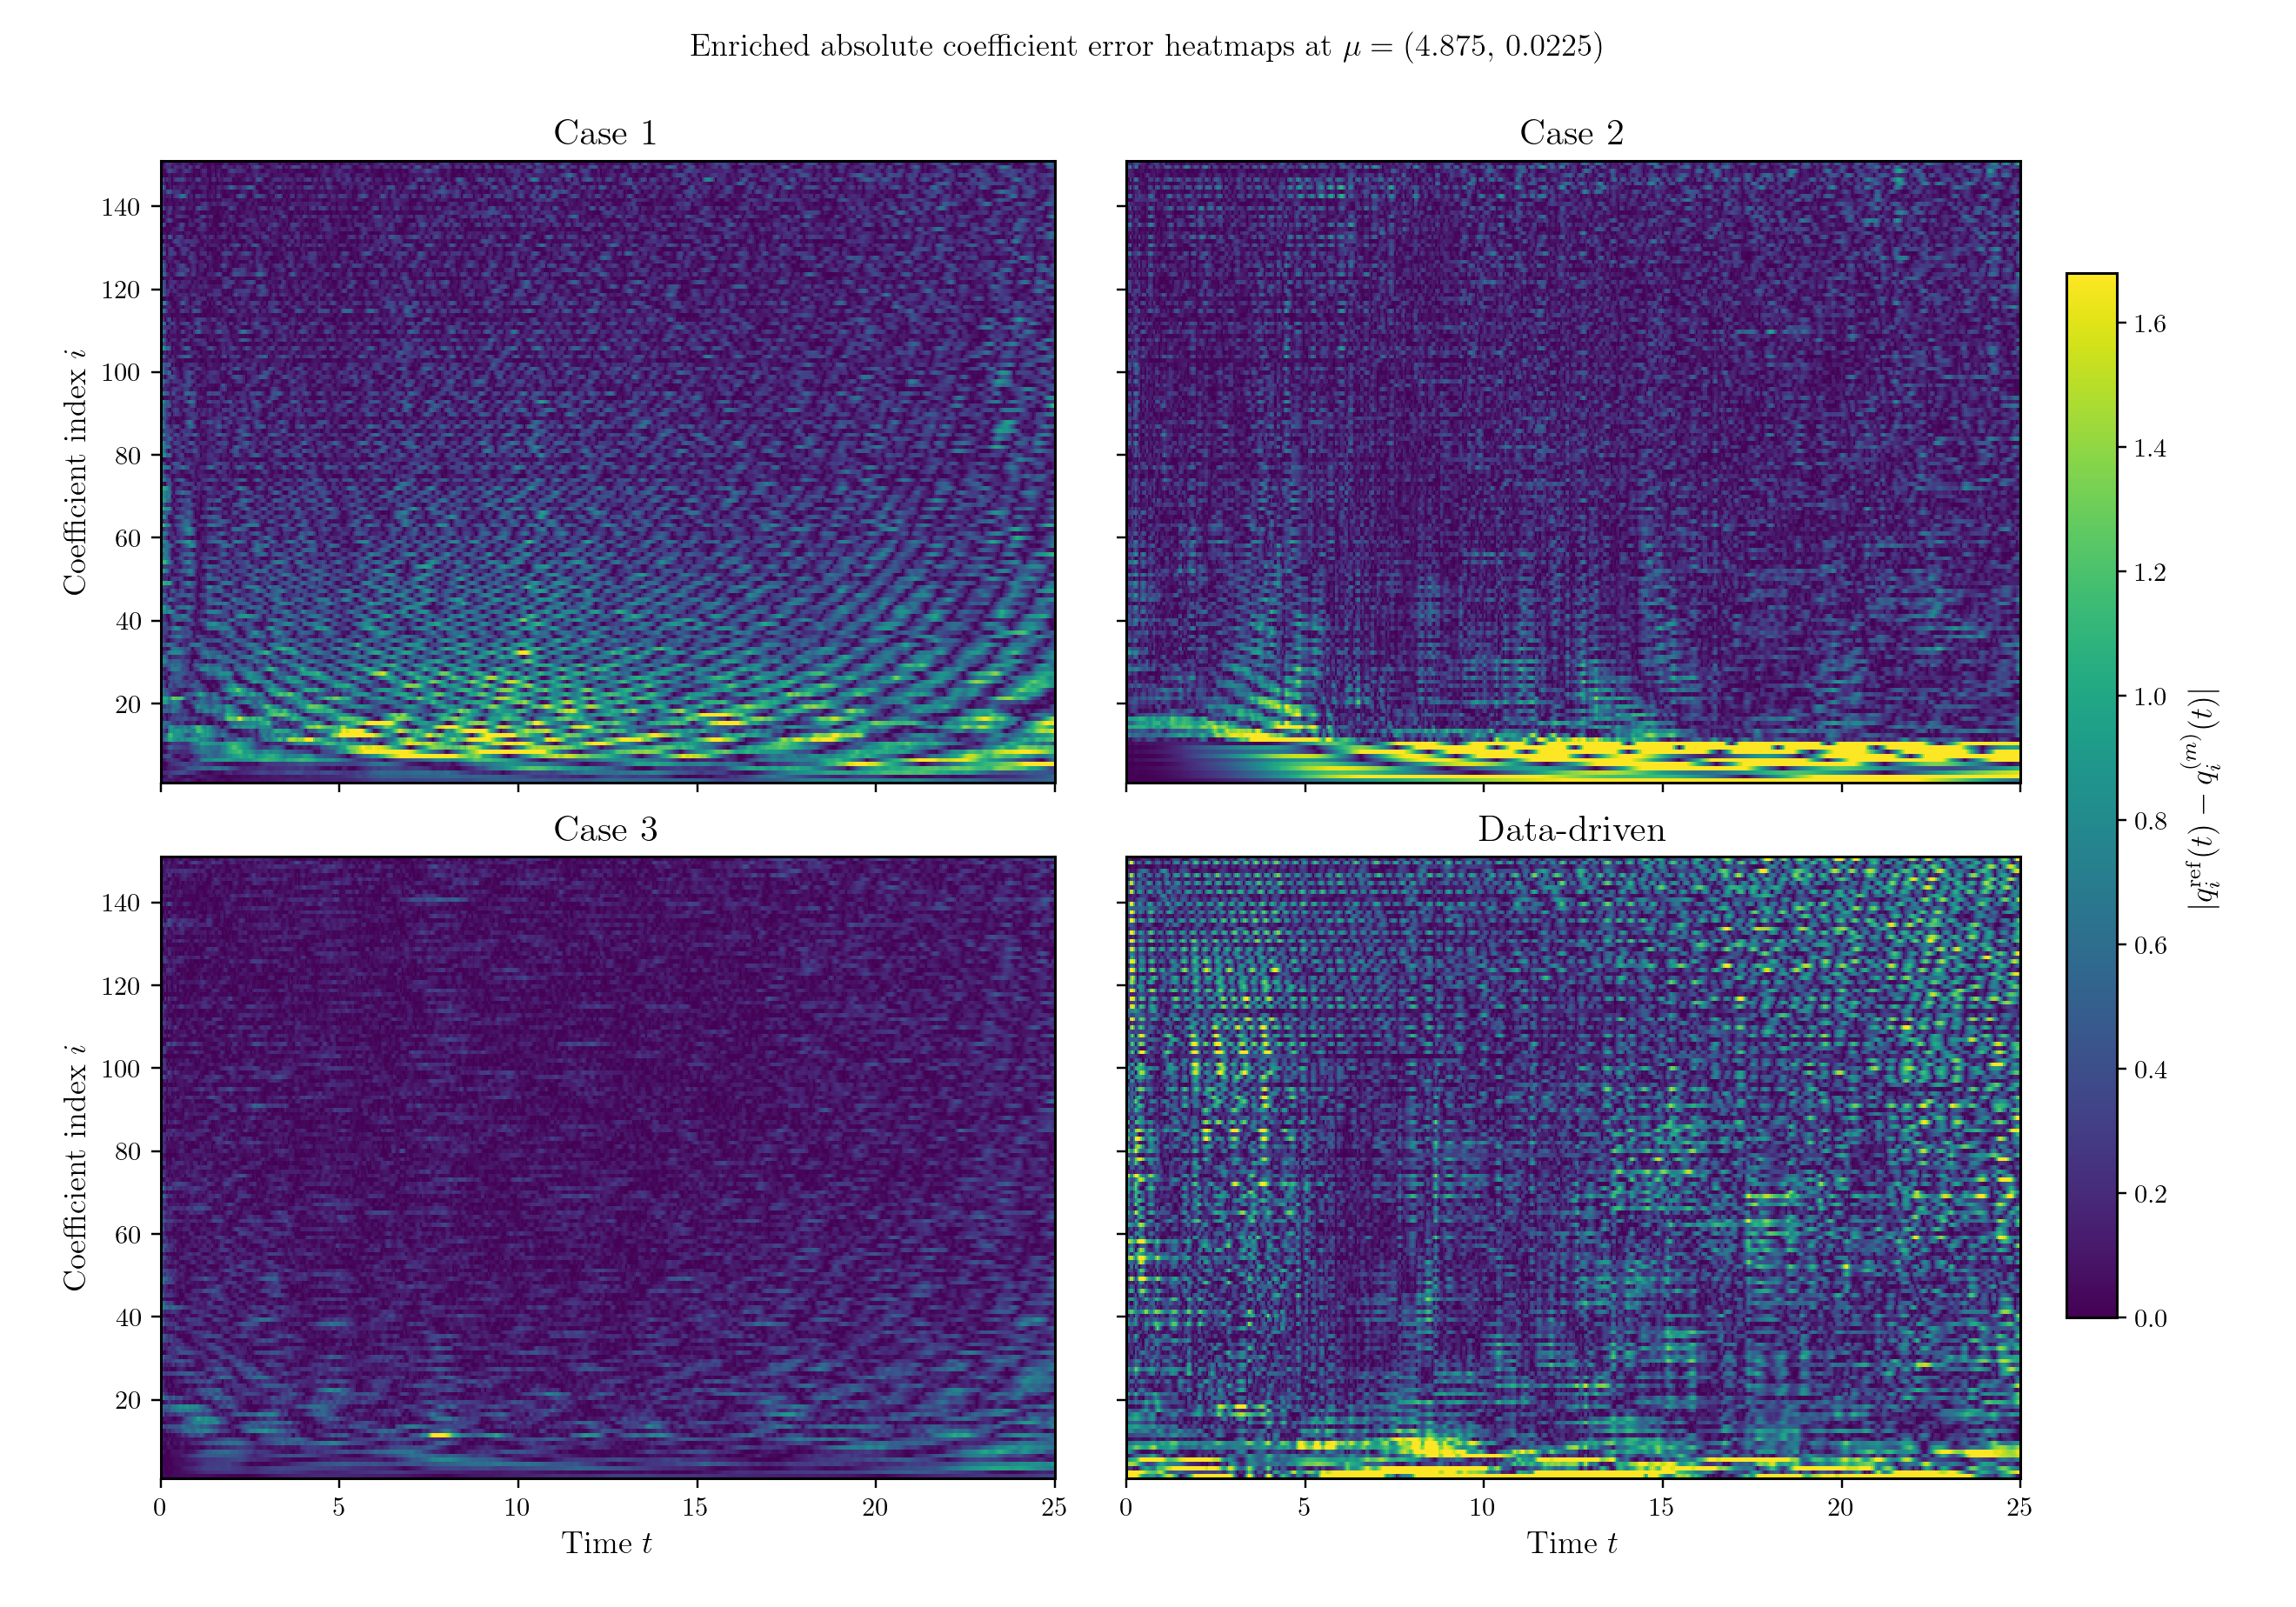
\includegraphics[width=0.98\textwidth]{Figures/coeff_errors/enriched_mu1_4.875_mu2_0.0225_coeff_abs_heatmap_grid.png}
\caption{Enriched stage: absolute coefficient error heatmaps at $\bm\mu^{(v)}$.}
\label{fig:hm_enriched_abs_verif}
\end{figure}

\begin{figure}[H]
\centering
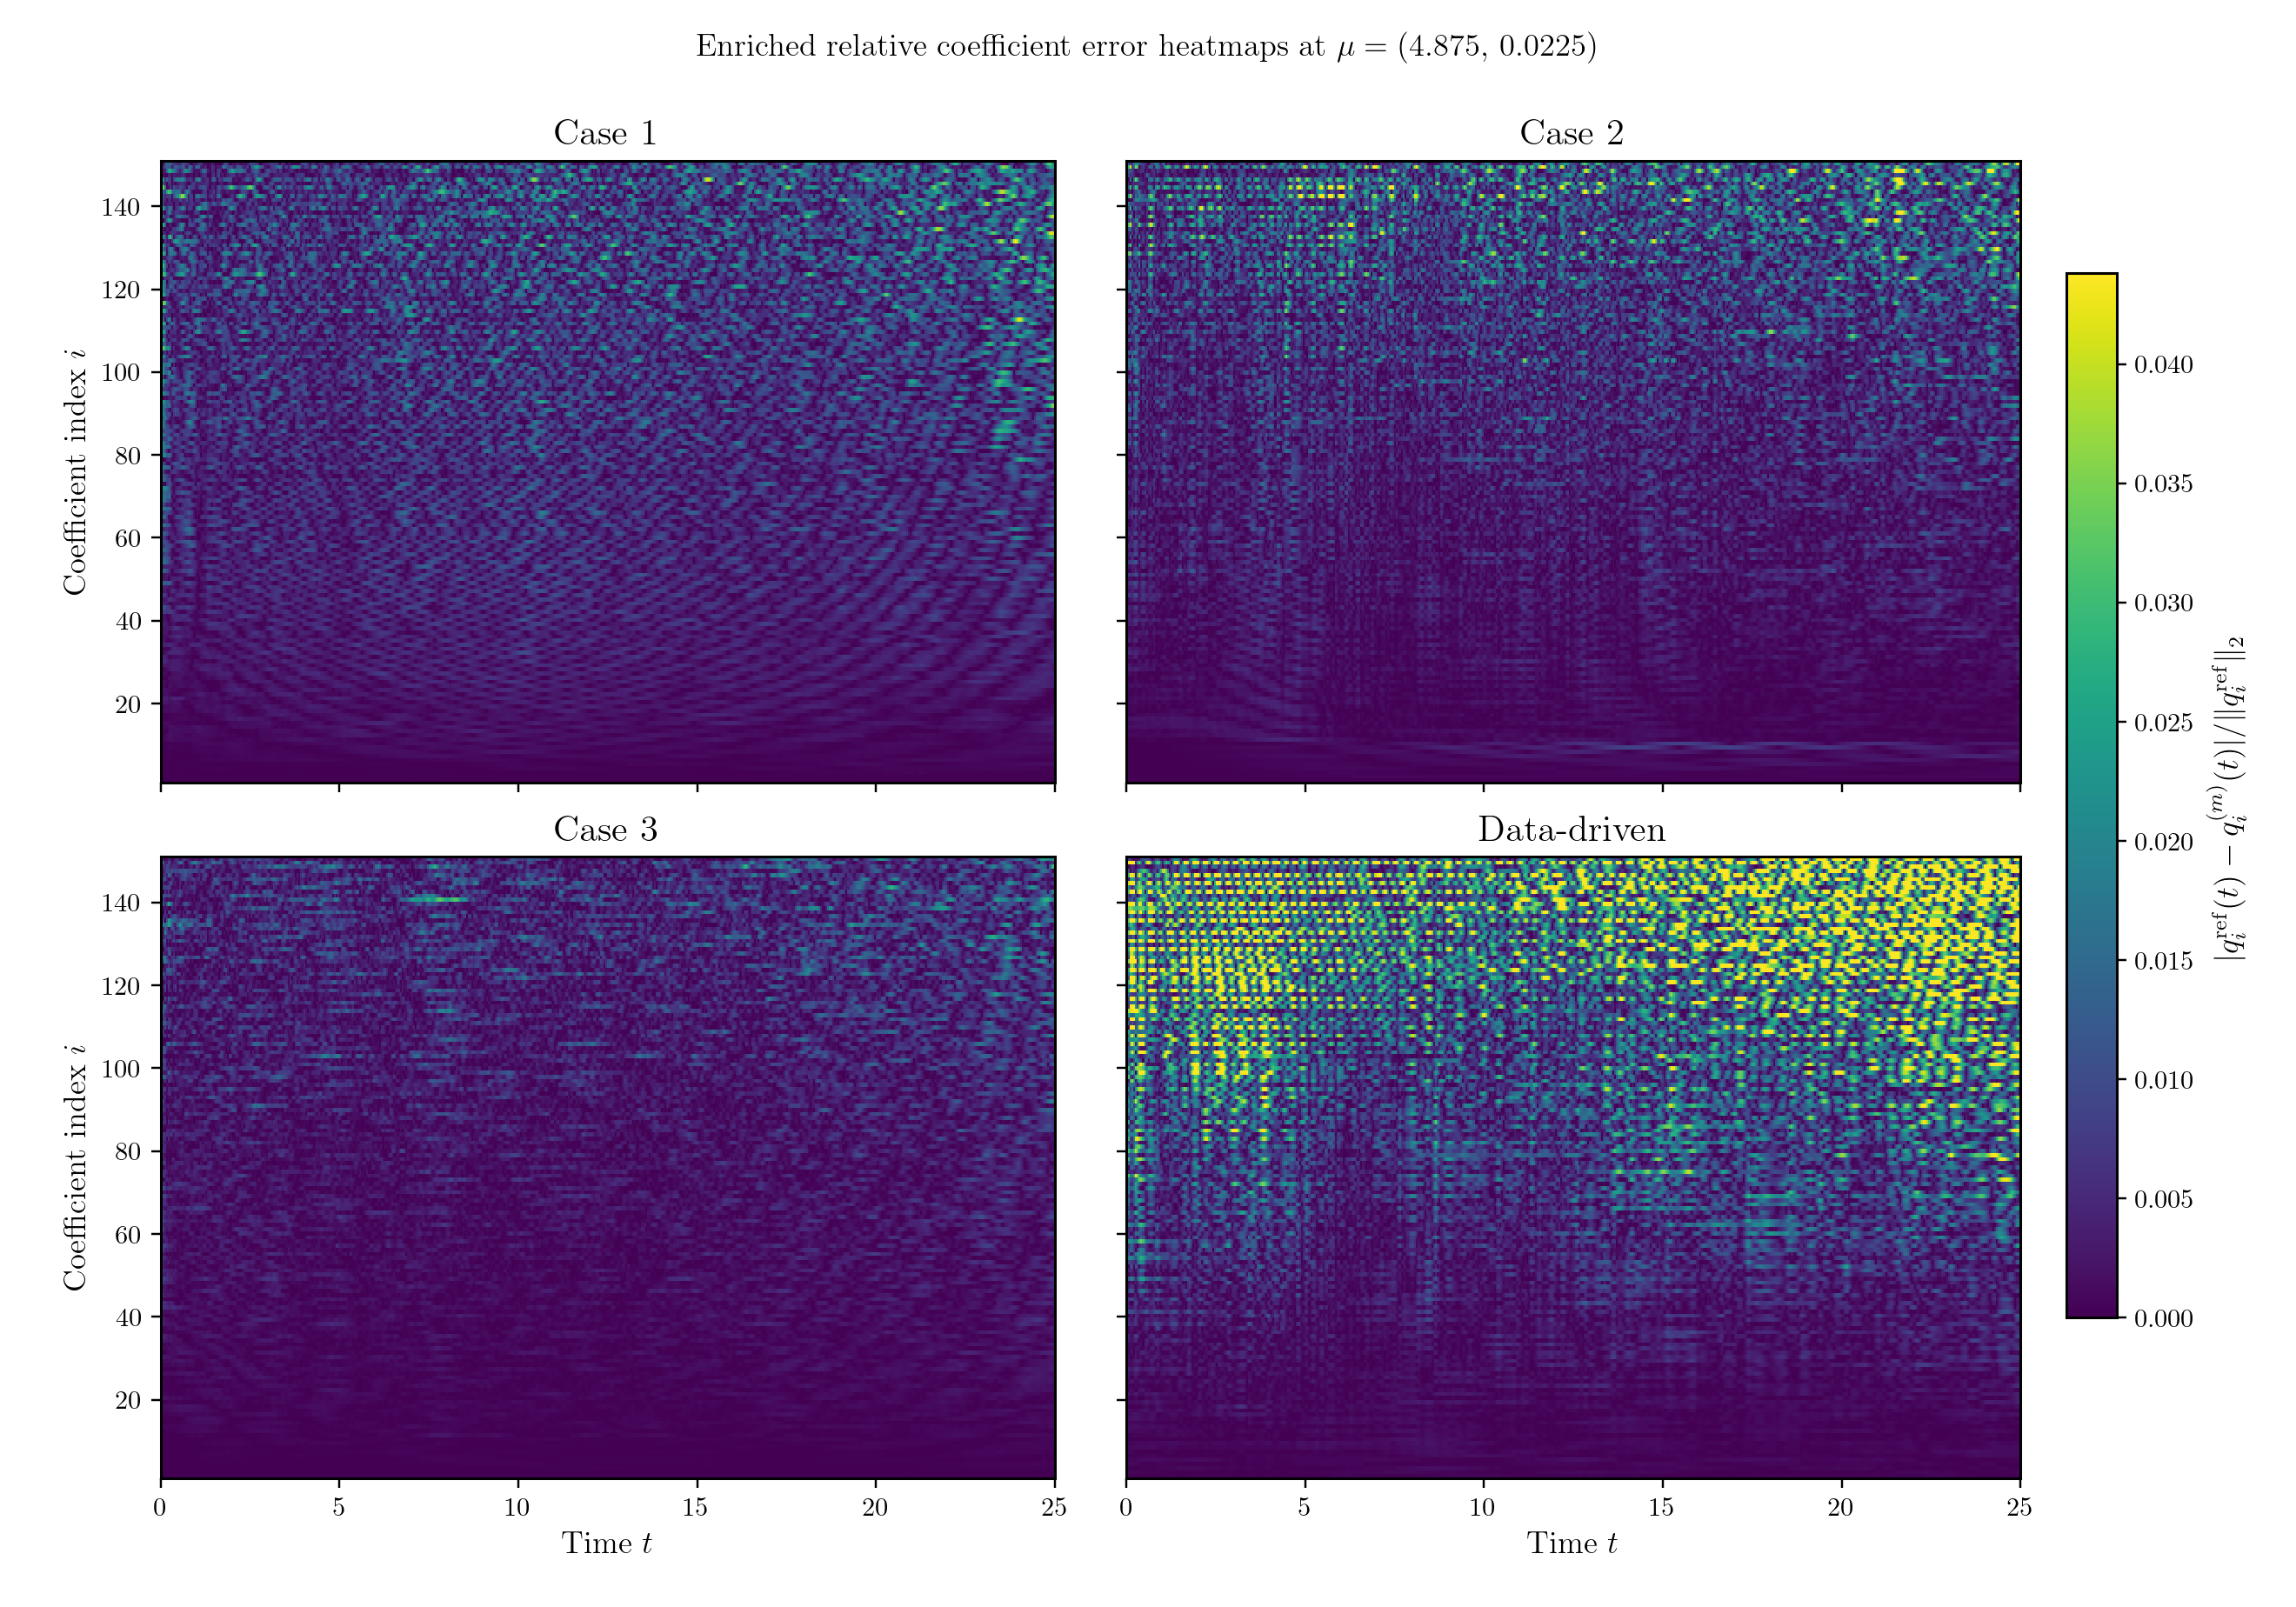
\includegraphics[width=0.98\textwidth]{Figures/coeff_errors/enriched_mu1_4.875_mu2_0.0225_coeff_rel_heatmap_grid.png}
\caption{Enriched stage: relative coefficient error heatmaps at $\bm\mu^{(v)}$.}
\label{fig:hm_enriched_rel_verif}
\end{figure}

\begin{figure}[H]
\centering
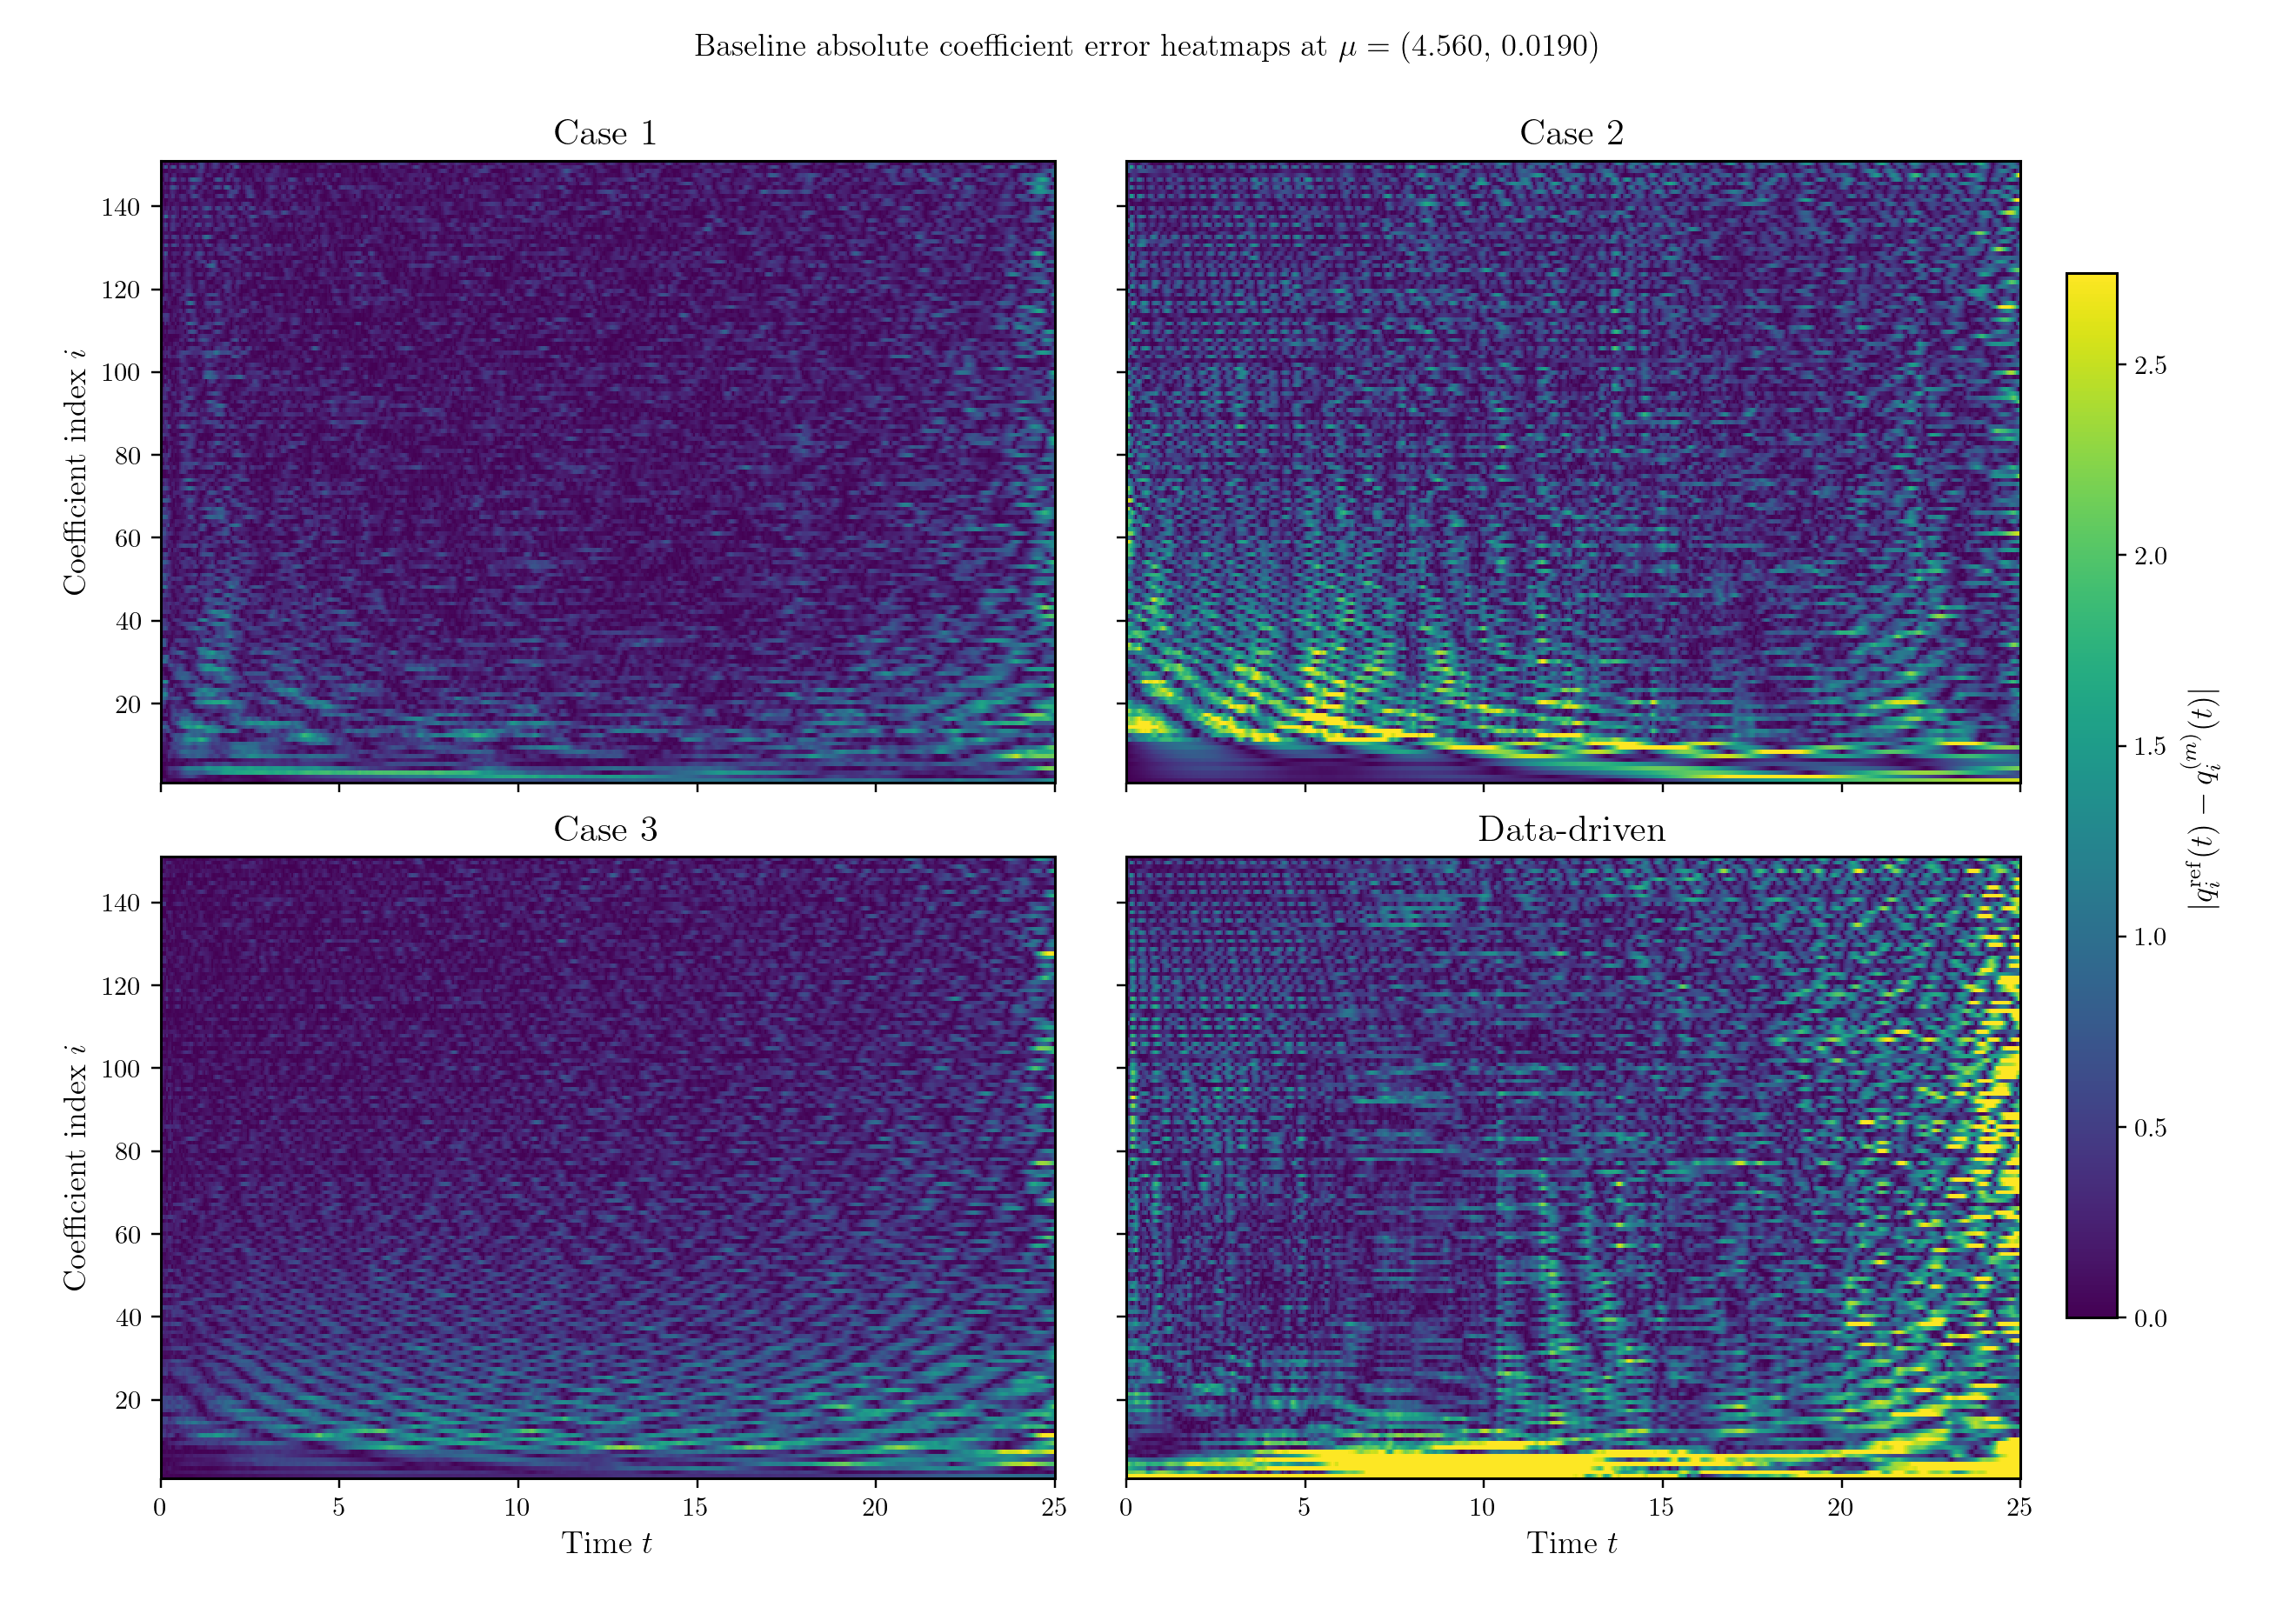
\includegraphics[width=0.98\textwidth]{Figures/coeff_errors/baseline_mu1_4.560_mu2_0.0190_coeff_abs_heatmap_grid.png}
\caption{Baseline stage: absolute coefficient error heatmaps at $\bm\mu^{(1)}=(4.56,0.019)$.}
\label{fig:hm_baseline_abs_mu1}
\end{figure}

\begin{figure}[H]
\centering
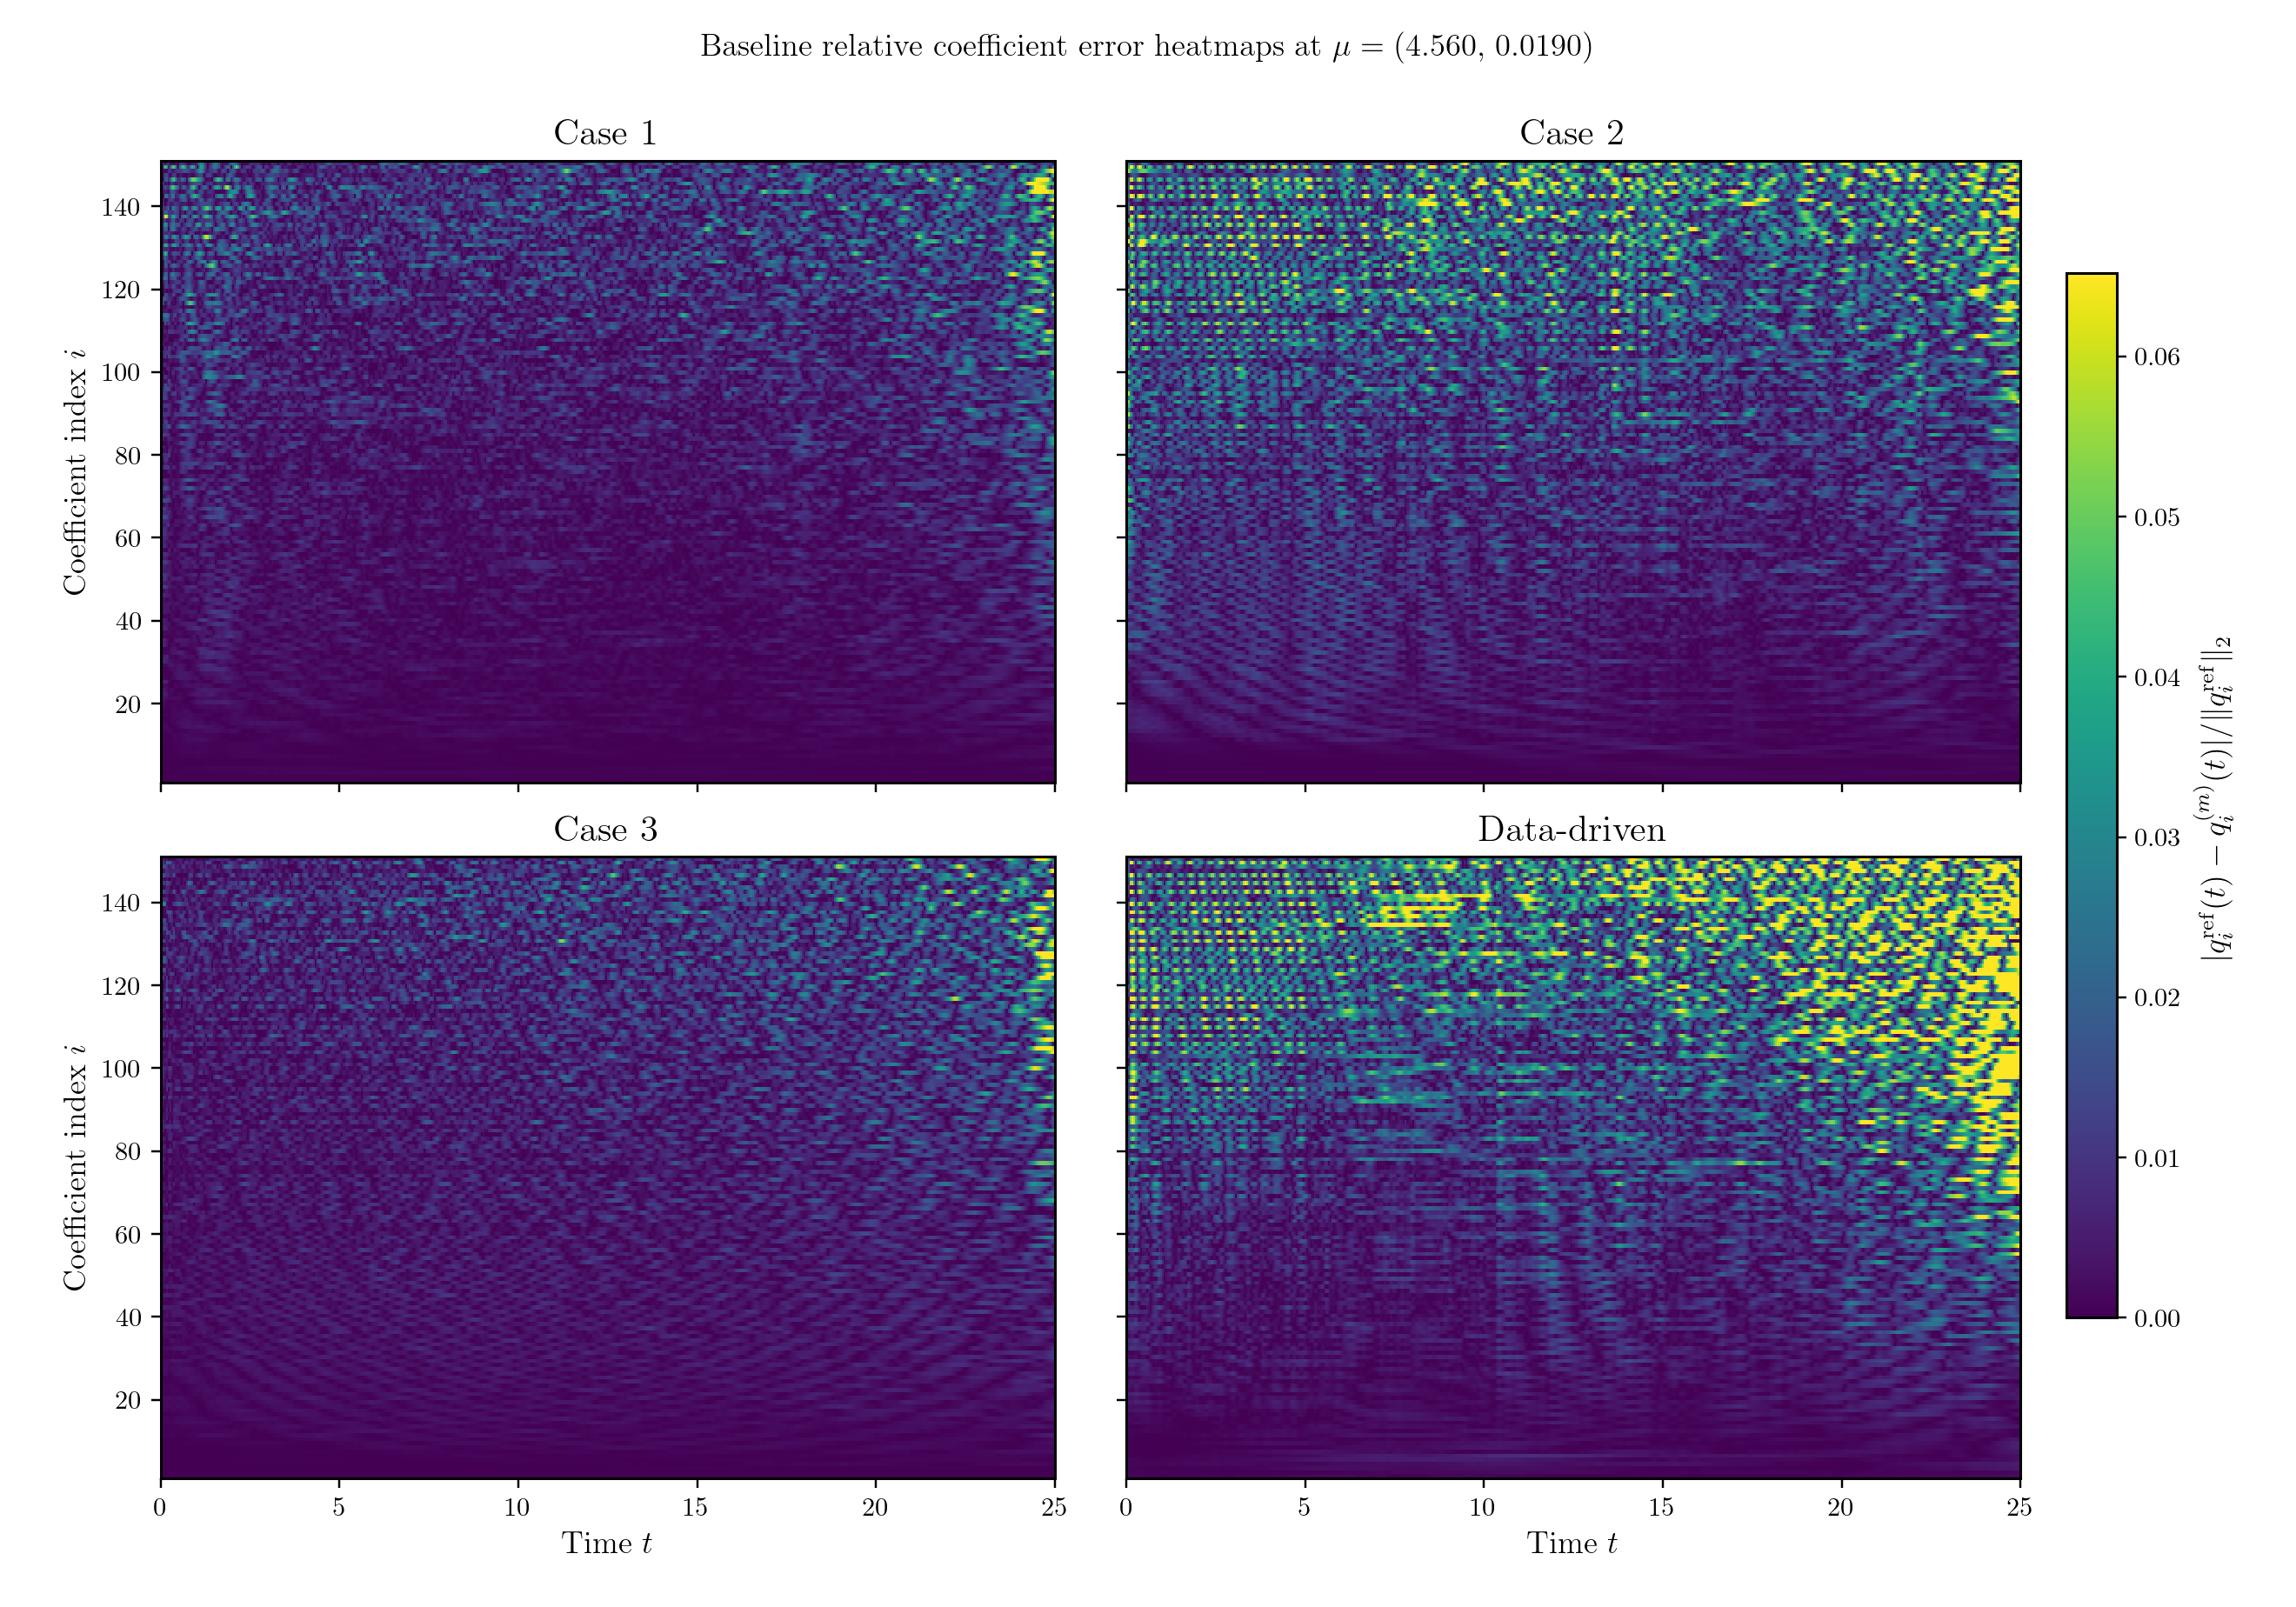
\includegraphics[width=0.98\textwidth]{Figures/coeff_errors/baseline_mu1_4.560_mu2_0.0190_coeff_rel_heatmap_grid.png}
\caption{Baseline stage: relative coefficient error heatmaps at $\bm\mu^{(1)}=(4.56,0.019)$.}
\label{fig:hm_baseline_rel_mu1}
\end{figure}

\begin{figure}[H]
\centering
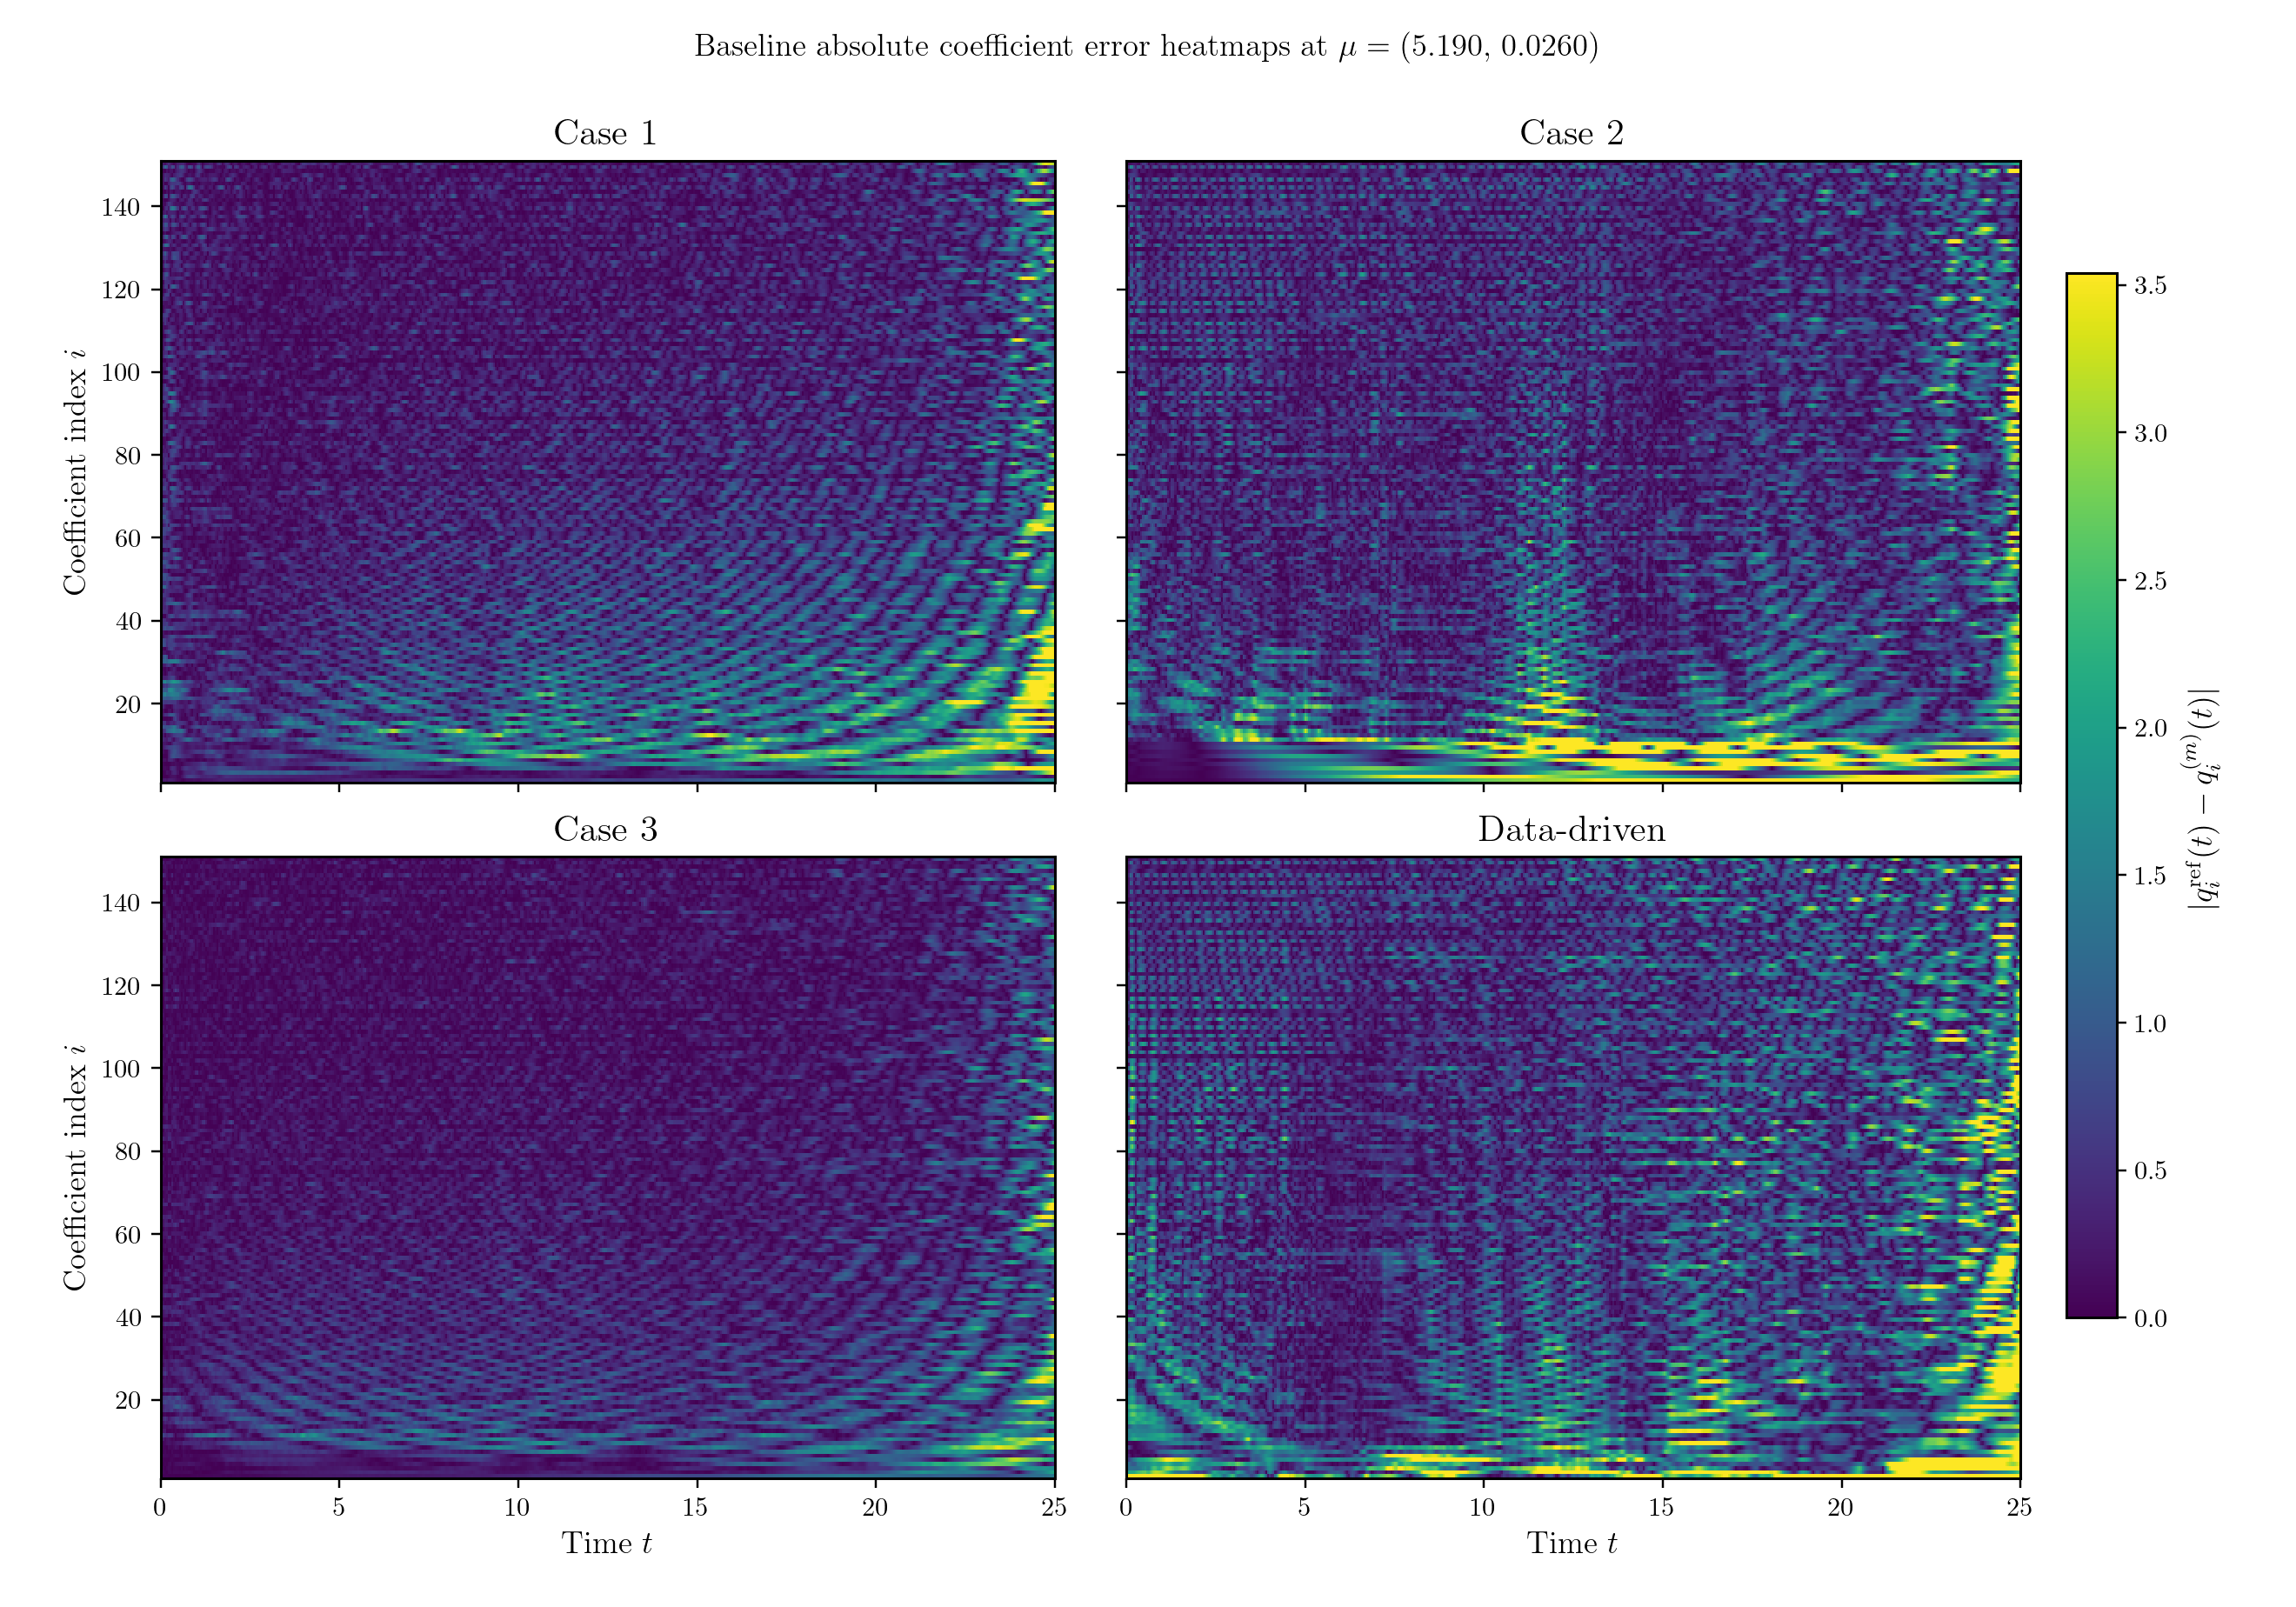
\includegraphics[width=0.98\textwidth]{Figures/coeff_errors/baseline_mu1_5.190_mu2_0.0260_coeff_abs_heatmap_grid.png}
\caption{Baseline stage: absolute coefficient error heatmaps at $\bm\mu^{(2)}=(5.19,0.026)$.}
\label{fig:hm_baseline_abs_mu2}
\end{figure}

\begin{figure}[H]
\centering
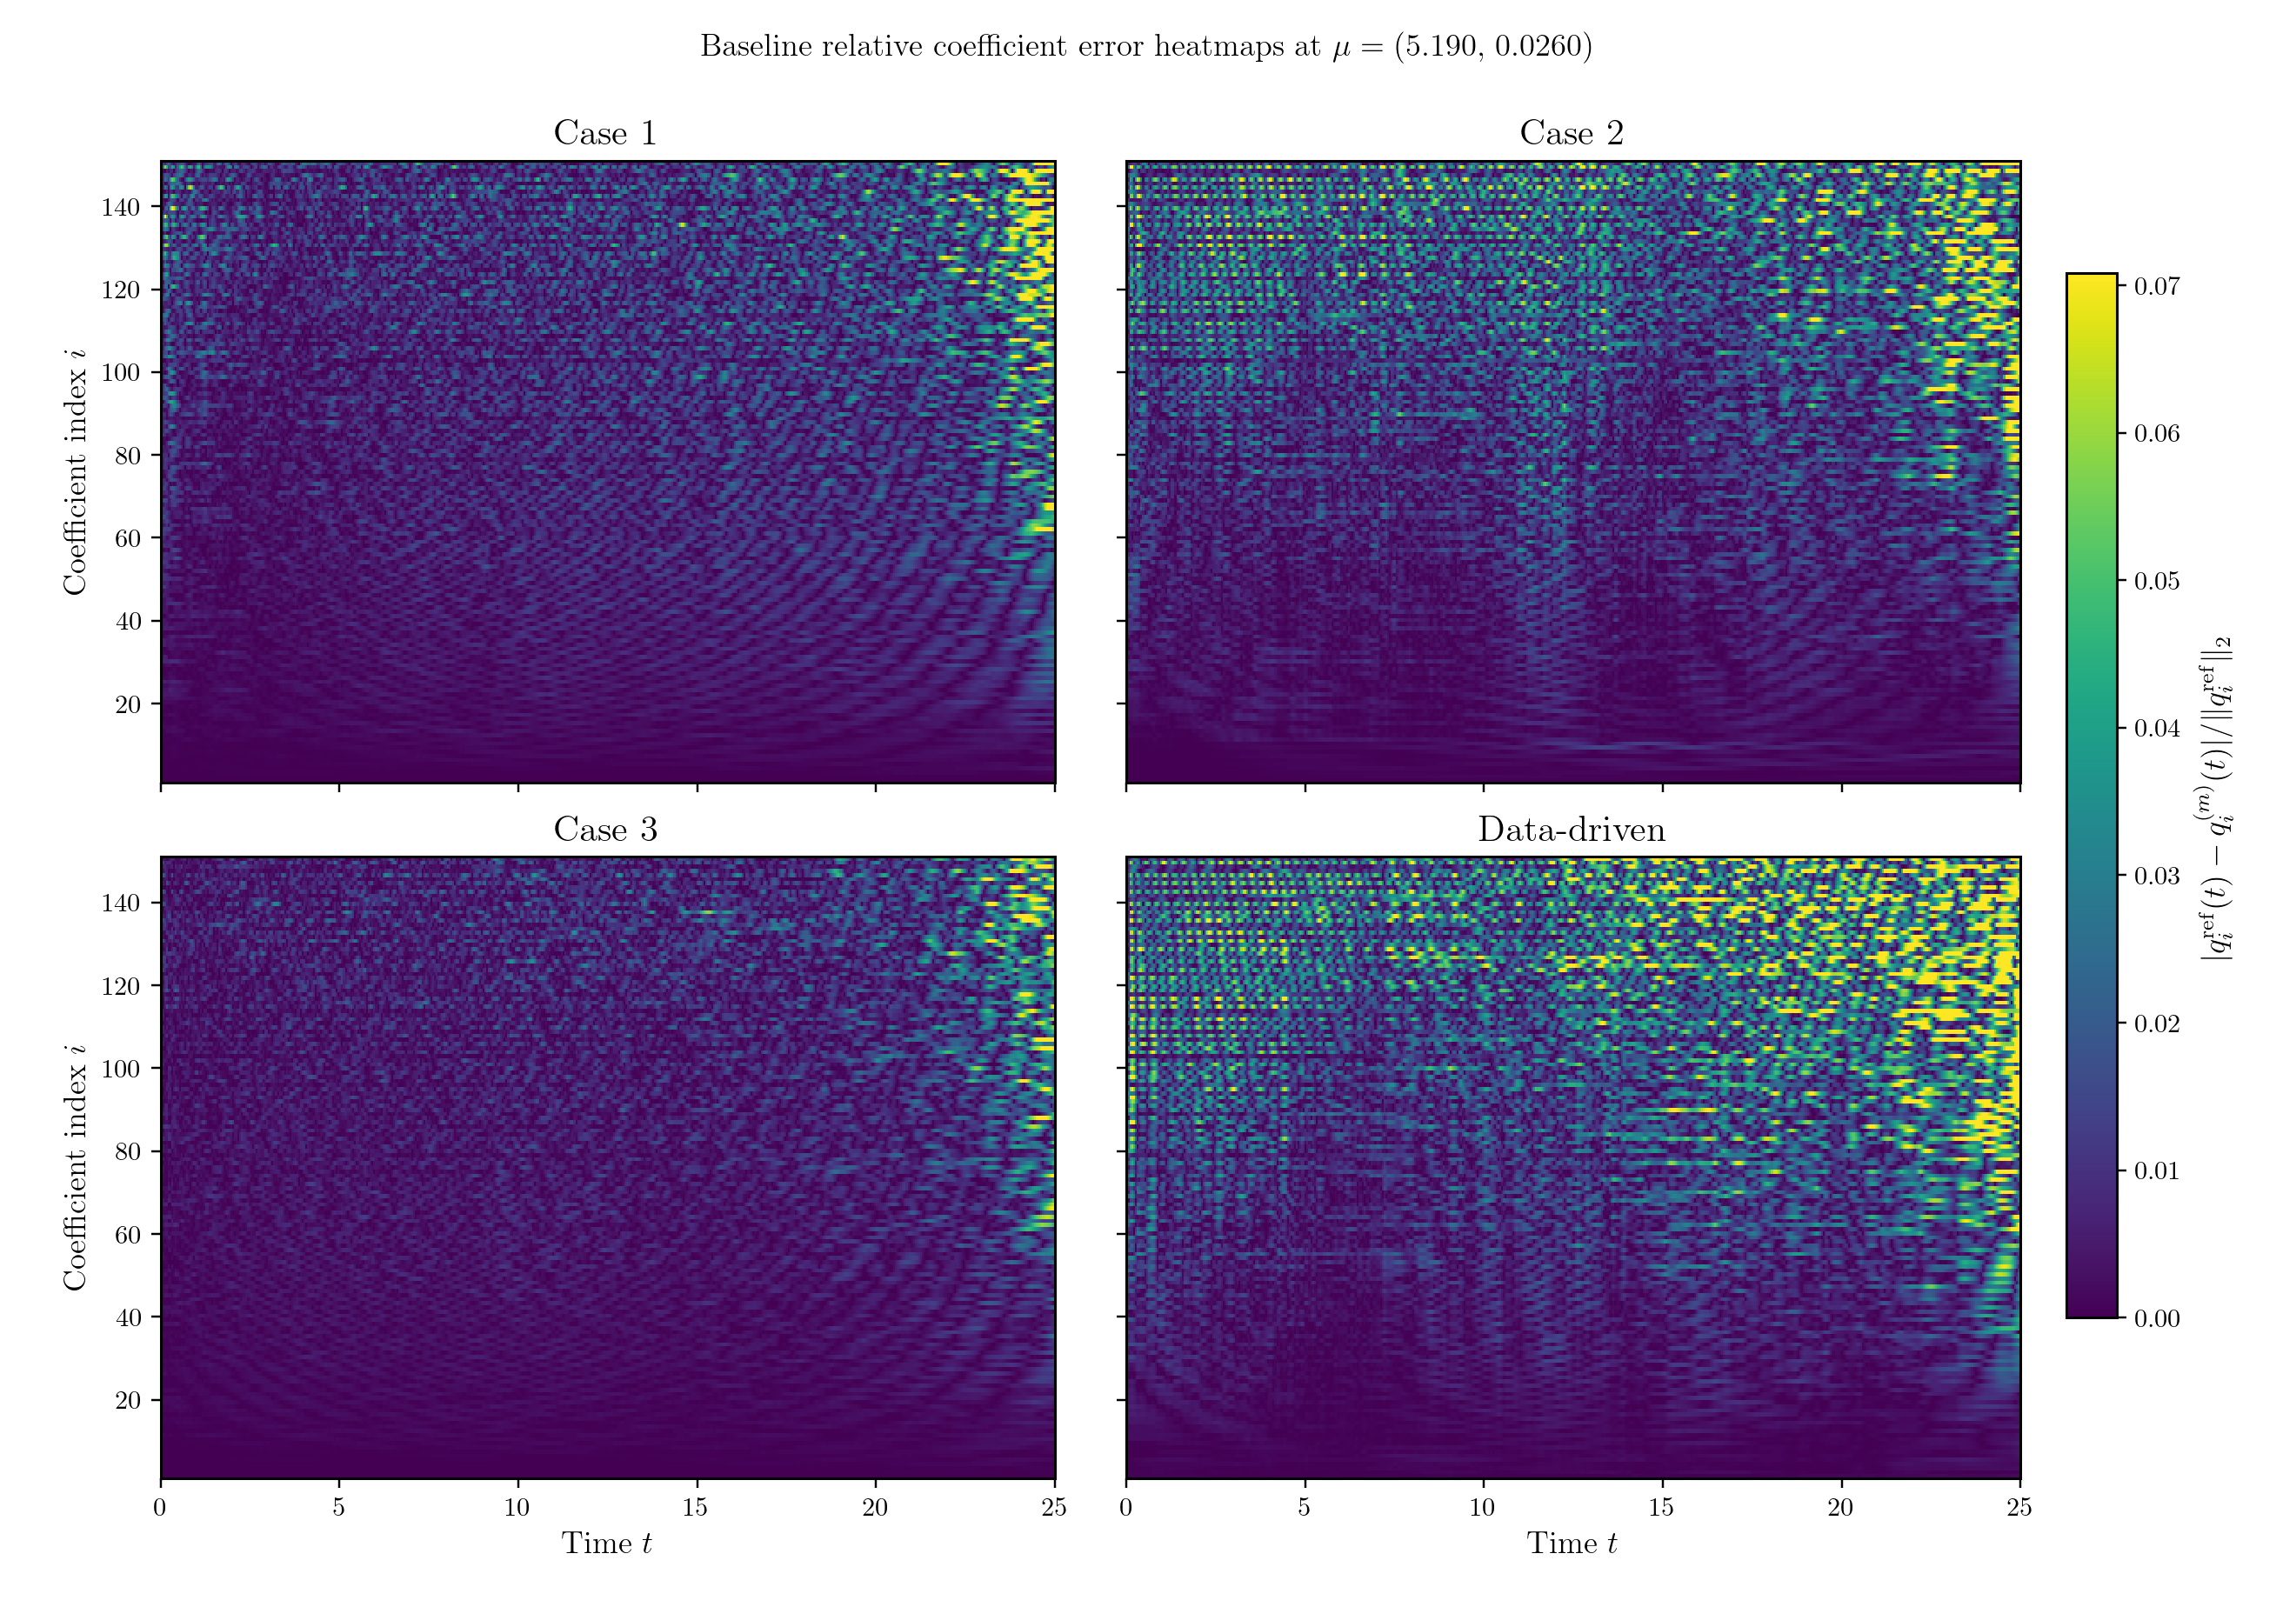
\includegraphics[width=0.98\textwidth]{Figures/coeff_errors/baseline_mu1_5.190_mu2_0.0260_coeff_rel_heatmap_grid.png}
\caption{Baseline stage: relative coefficient error heatmaps at $\bm\mu^{(2)}=(5.19,0.026)$.}
\label{fig:hm_baseline_rel_mu2}
\end{figure}

\begin{figure}[H]
\centering
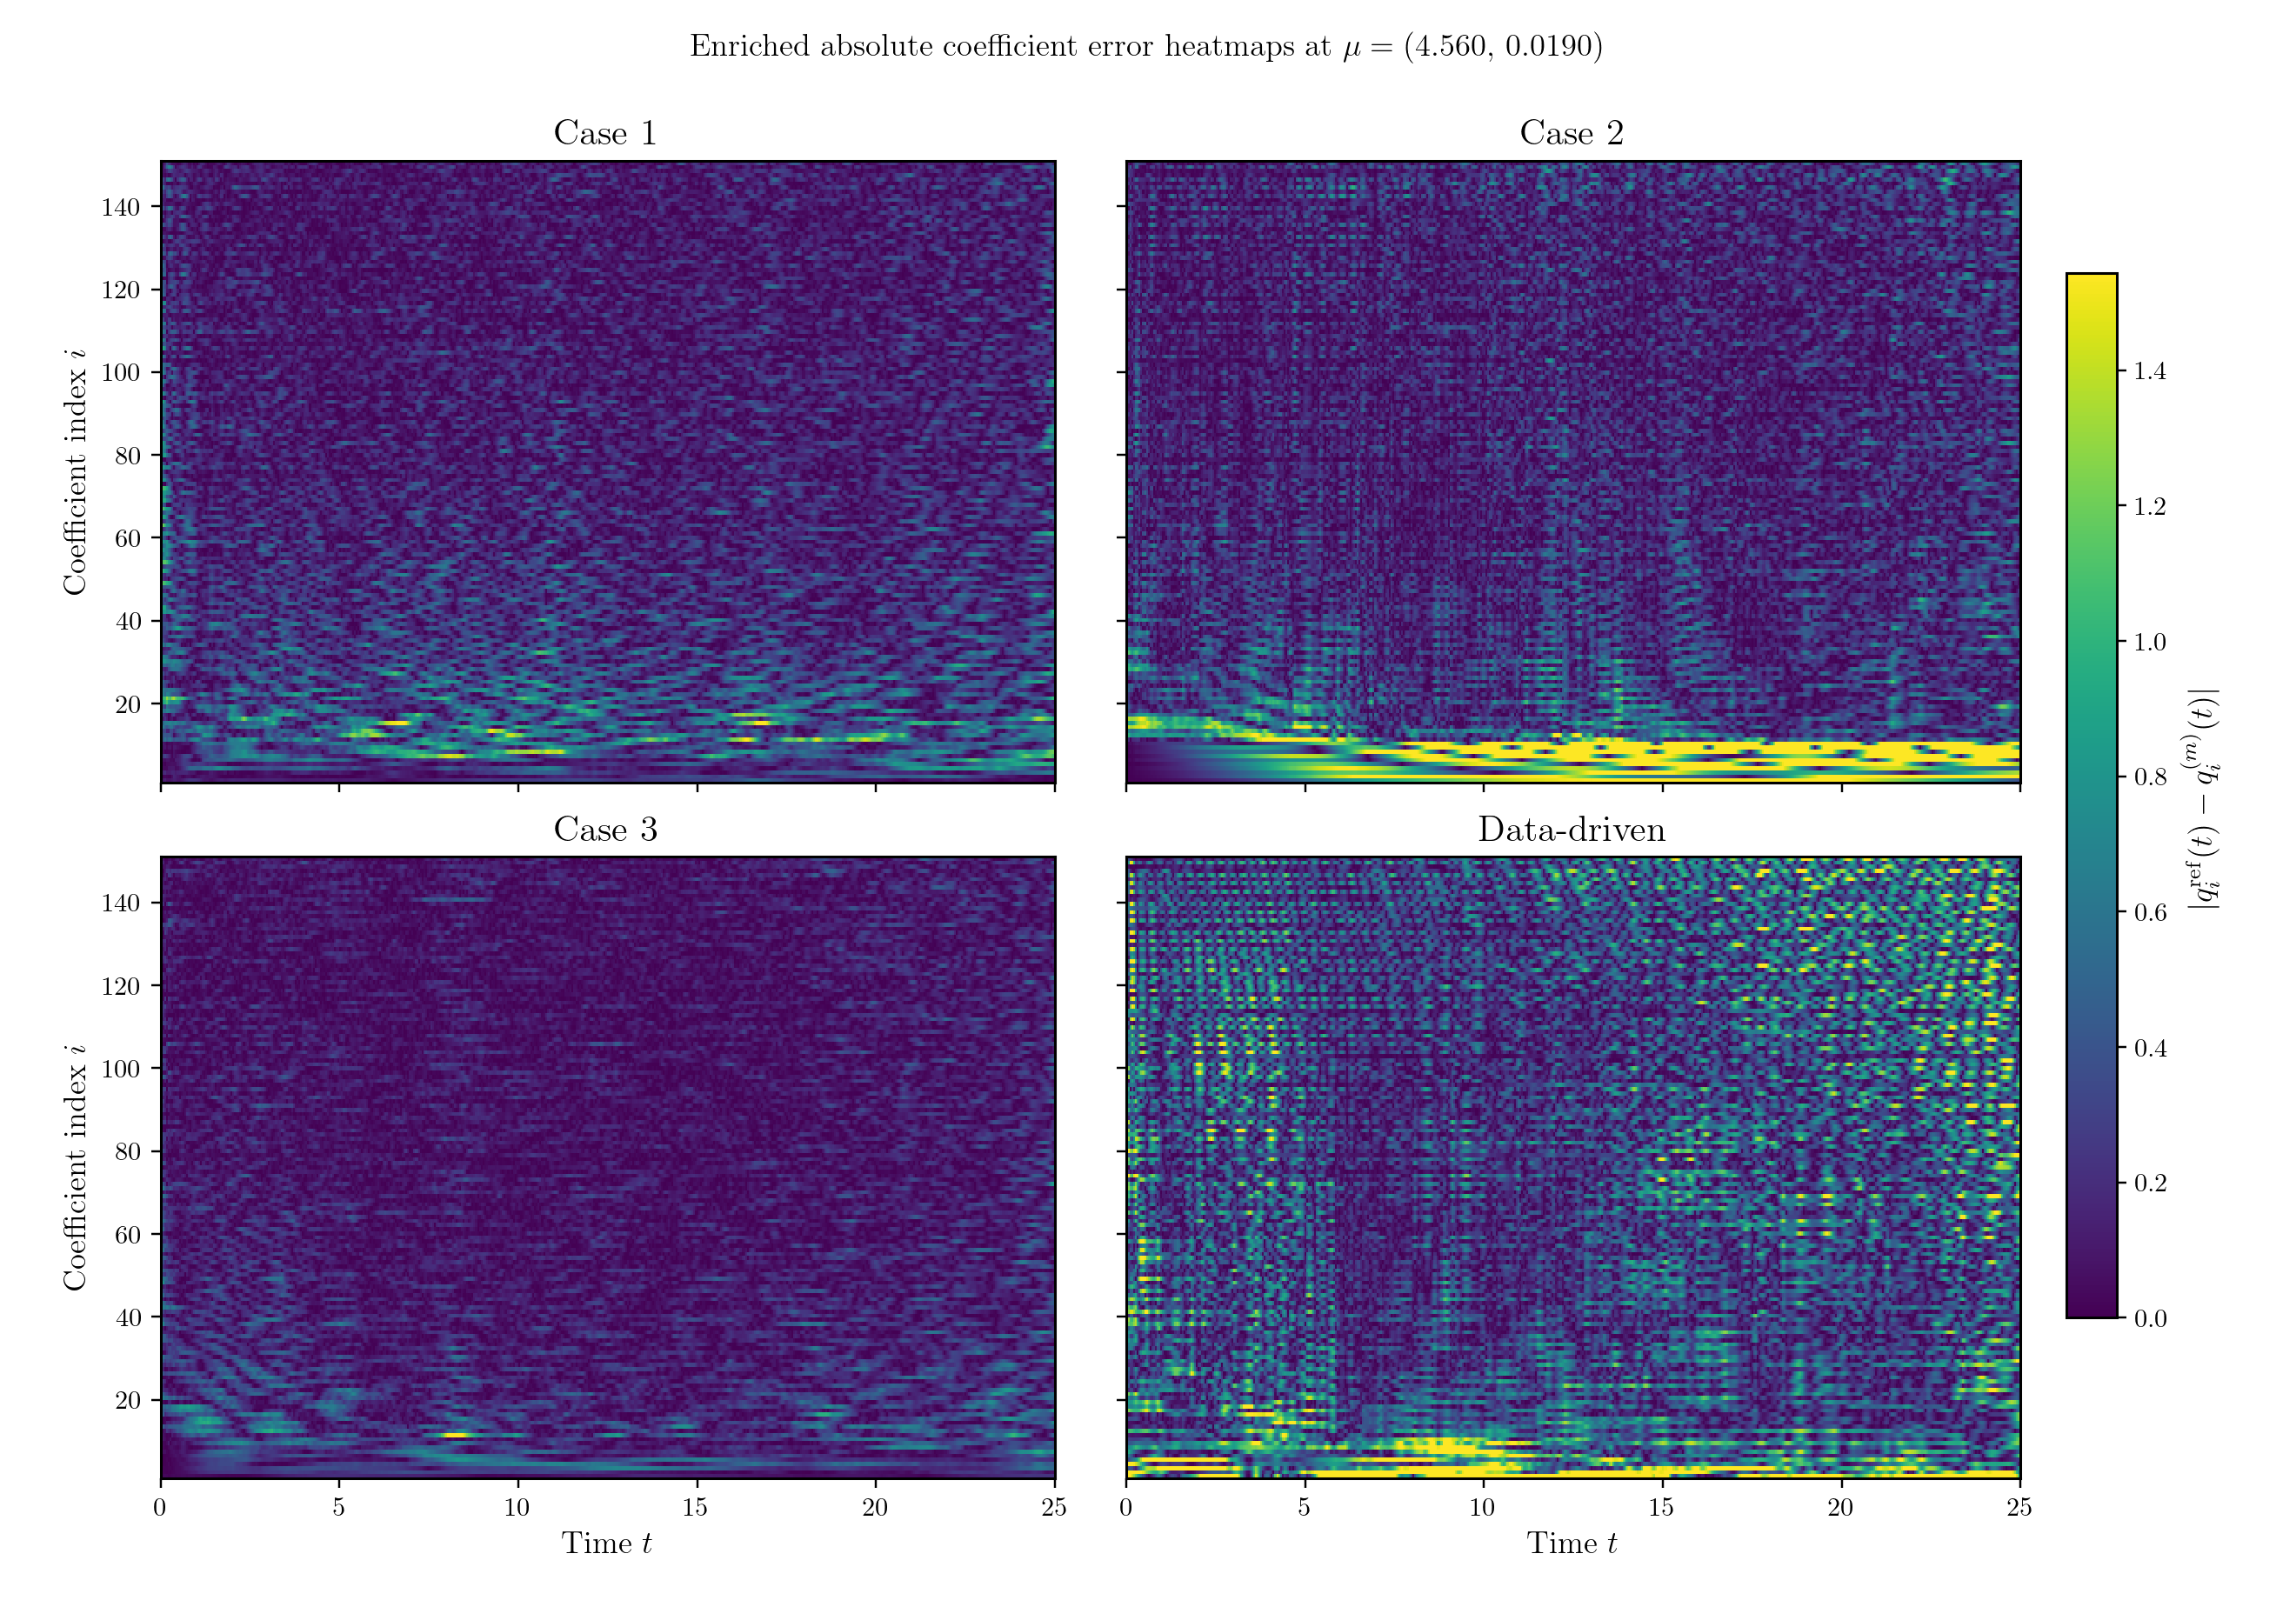
\includegraphics[width=0.98\textwidth]{Figures/coeff_errors/enriched_mu1_4.560_mu2_0.0190_coeff_abs_heatmap_grid.png}
\caption{Enriched stage: absolute coefficient error heatmaps at $\bm\mu^{(1)}=(4.56,0.019)$.}
\label{fig:hm_enriched_abs_mu1}
\end{figure}

\begin{figure}[H]
\centering
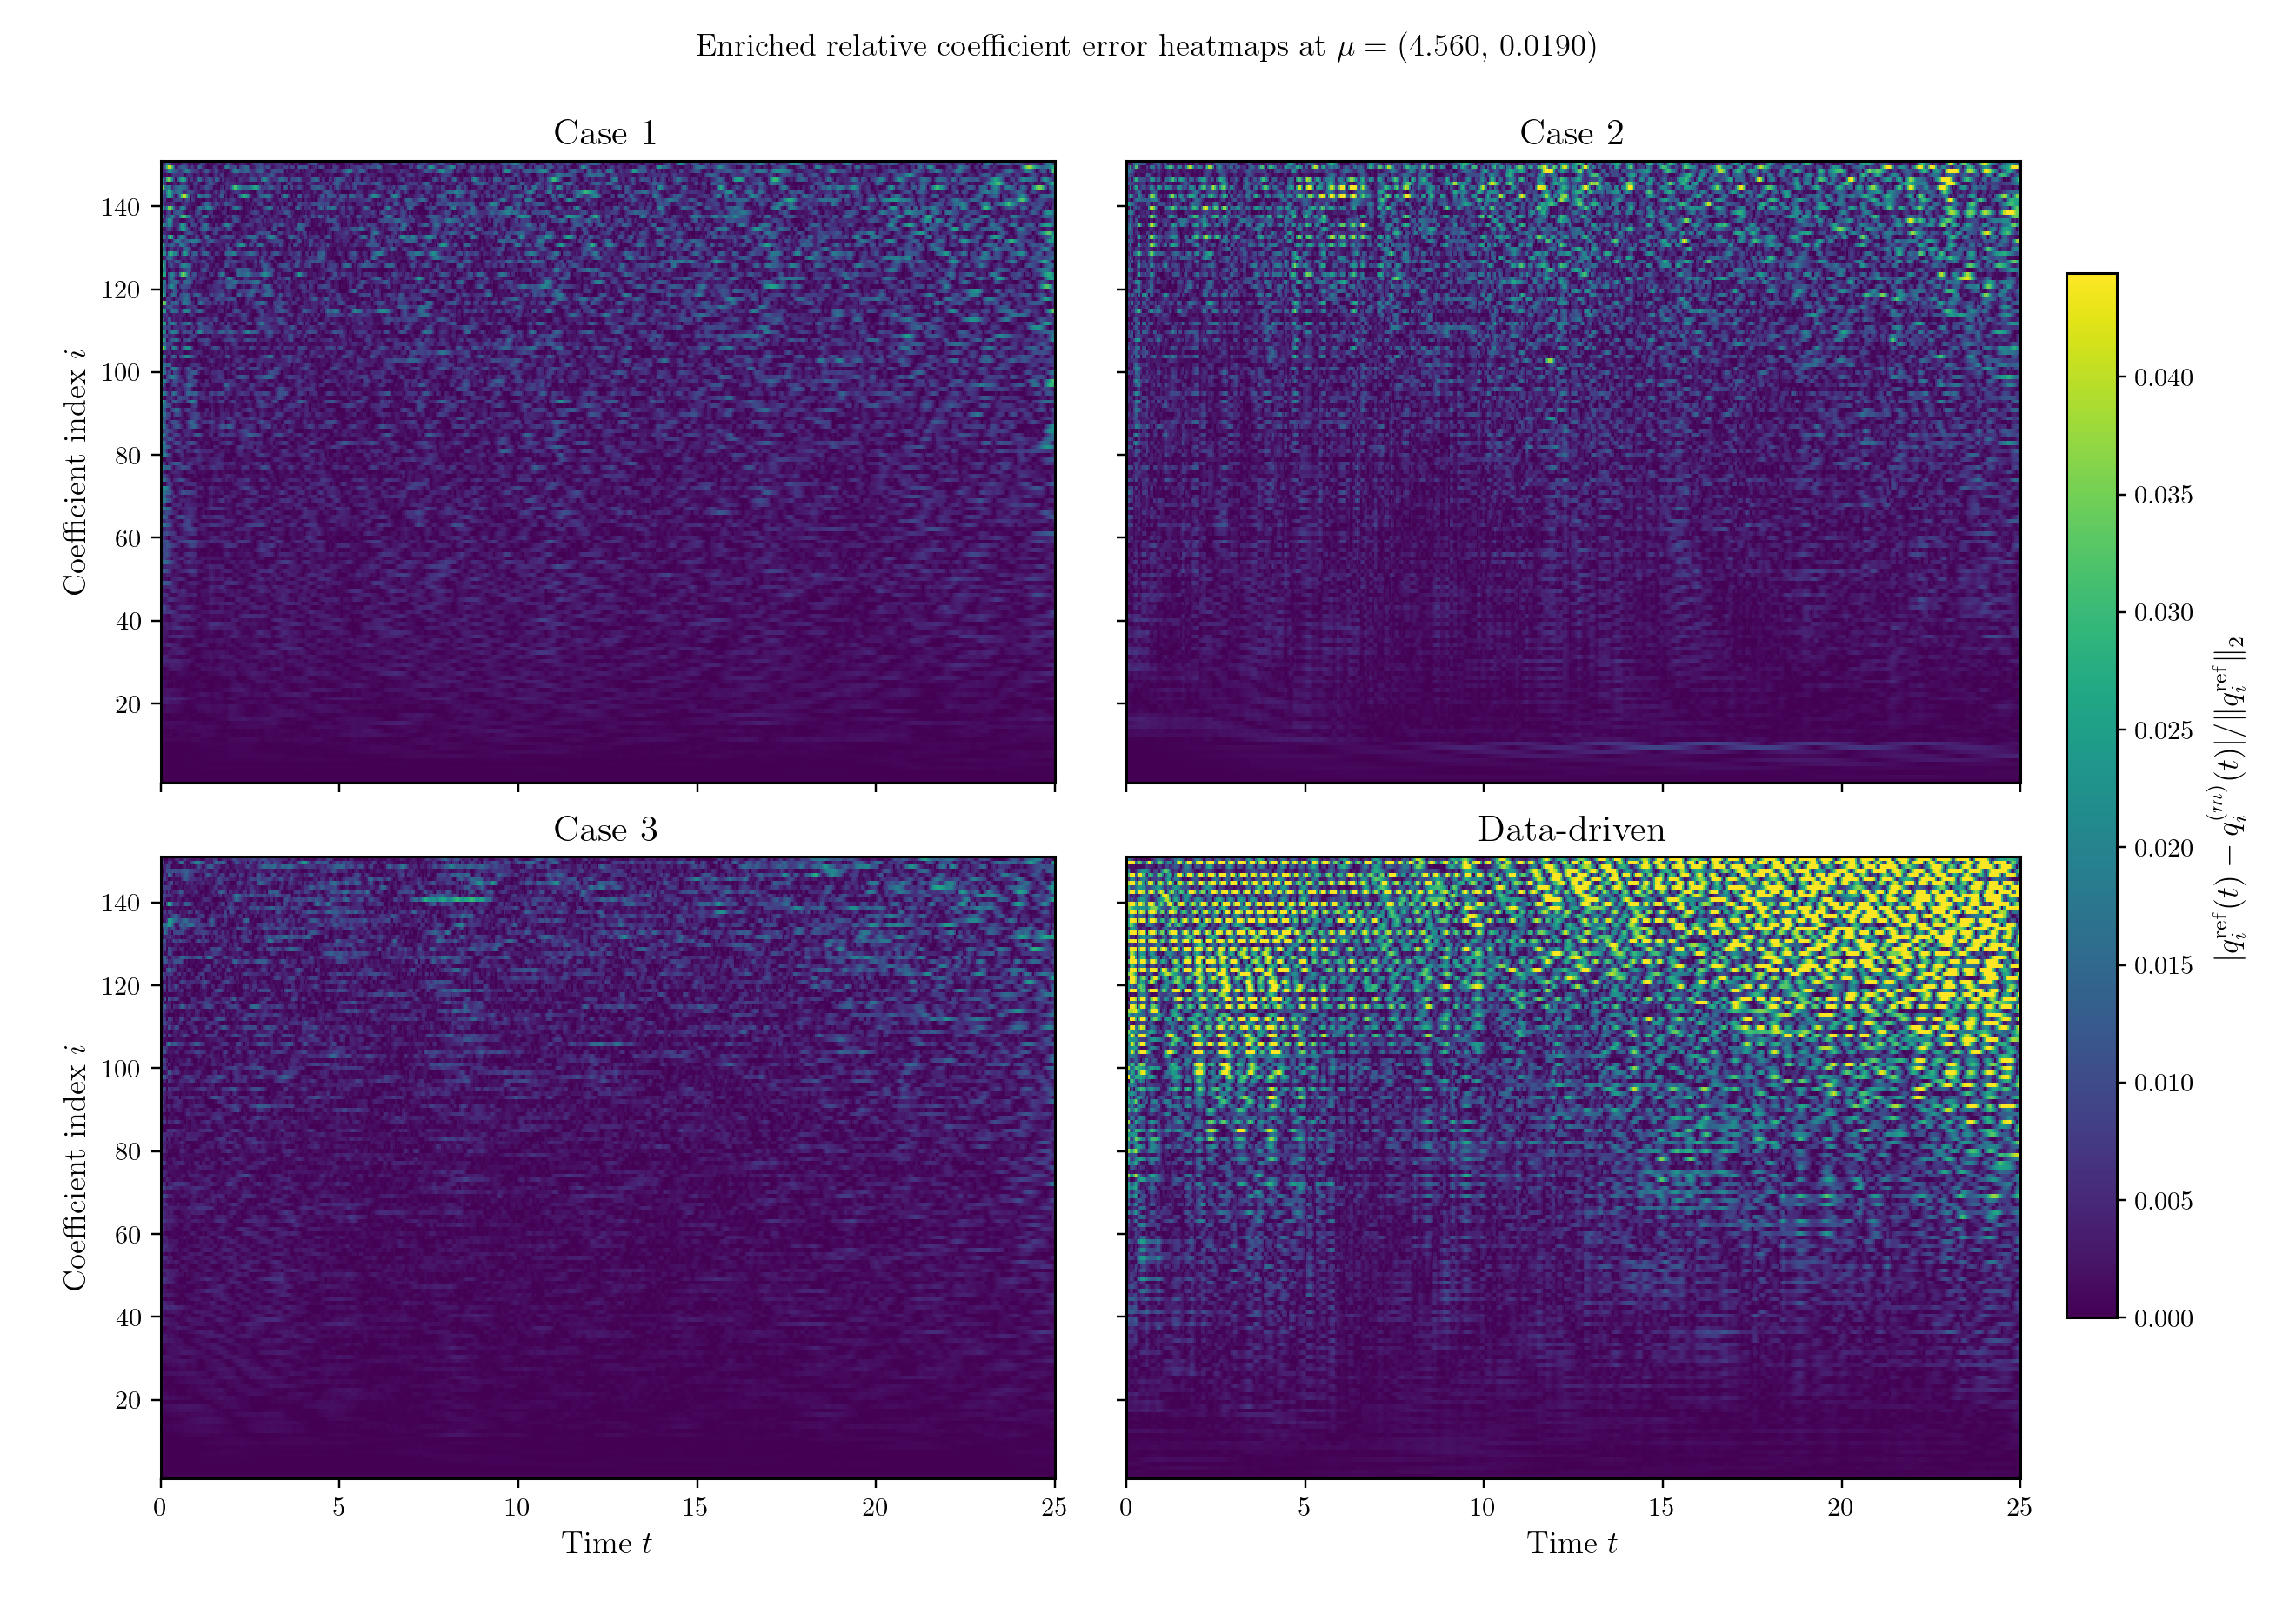
\includegraphics[width=0.98\textwidth]{Figures/coeff_errors/enriched_mu1_4.560_mu2_0.0190_coeff_rel_heatmap_grid.png}
\caption{Enriched stage: relative coefficient error heatmaps at $\bm\mu^{(1)}=(4.56,0.019)$.}
\label{fig:hm_enriched_rel_mu1}
\end{figure}

\begin{figure}[H]
\centering
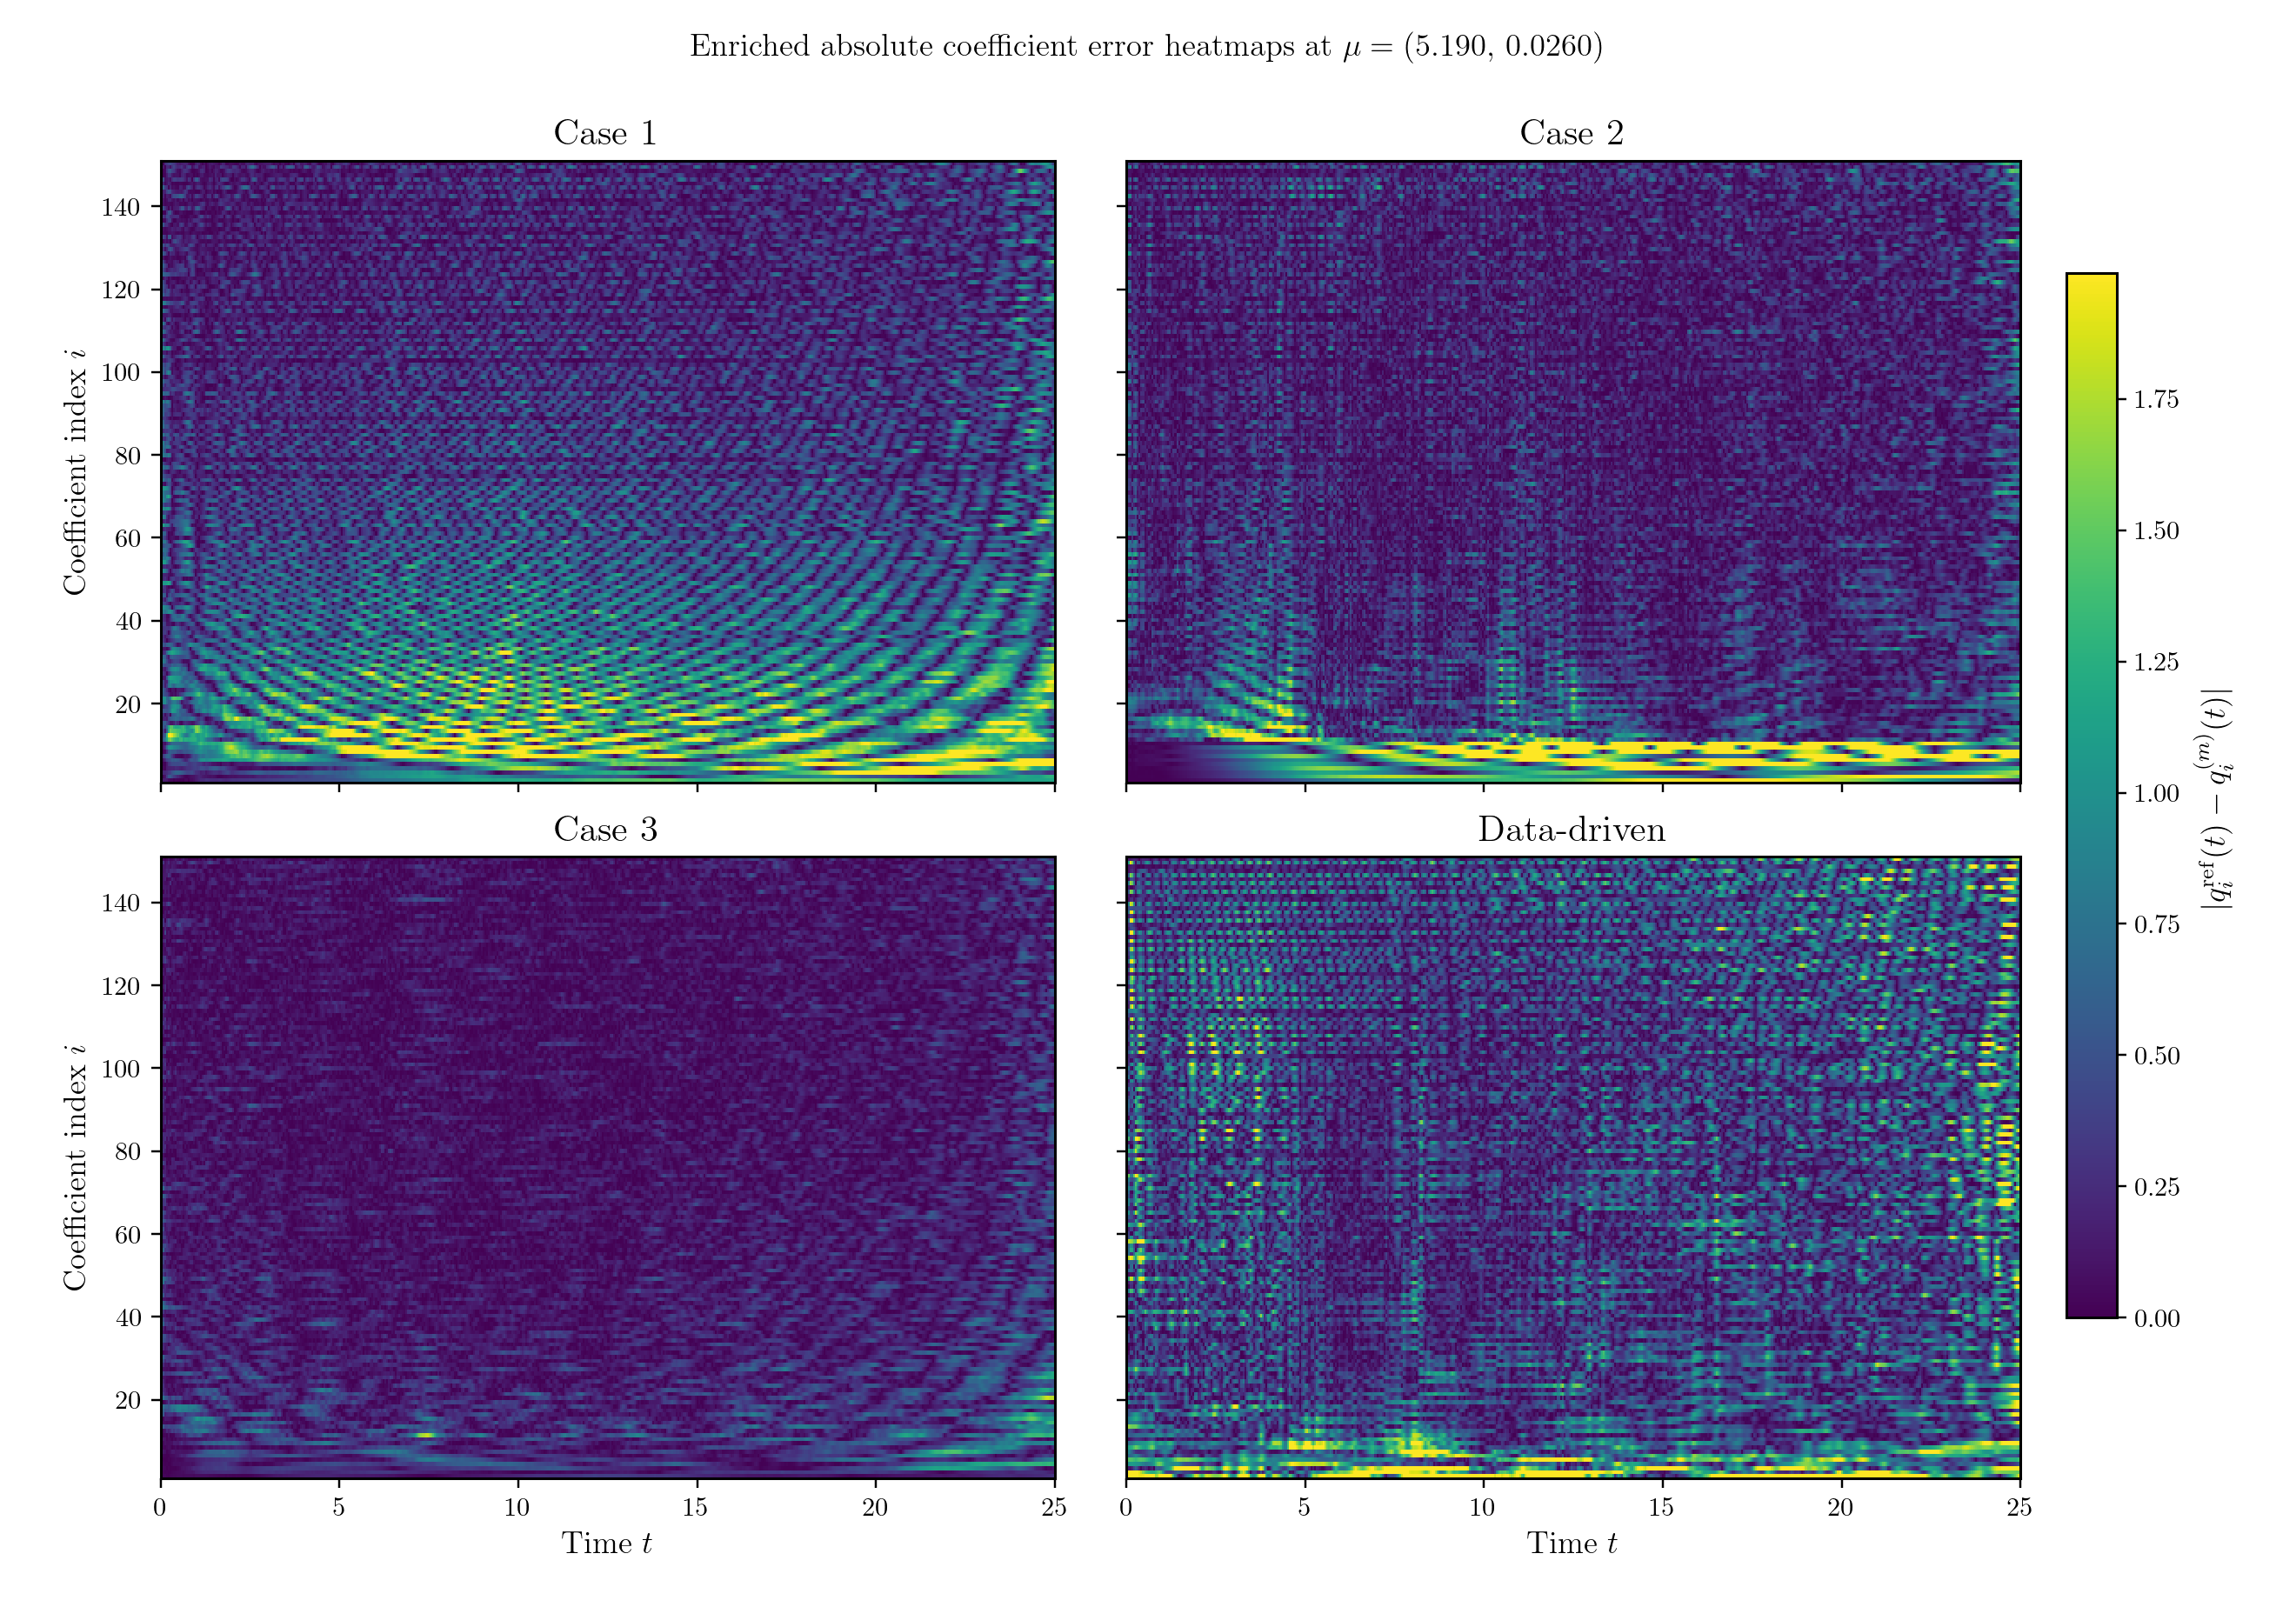
\includegraphics[width=0.98\textwidth]{Figures/coeff_errors/enriched_mu1_5.190_mu2_0.0260_coeff_abs_heatmap_grid.png}
\caption{Enriched stage: absolute coefficient error heatmaps at $\bm\mu^{(2)}=(5.19,0.026)$.}
\label{fig:hm_enriched_abs_mu2}
\end{figure}

\begin{figure}[H]
\centering
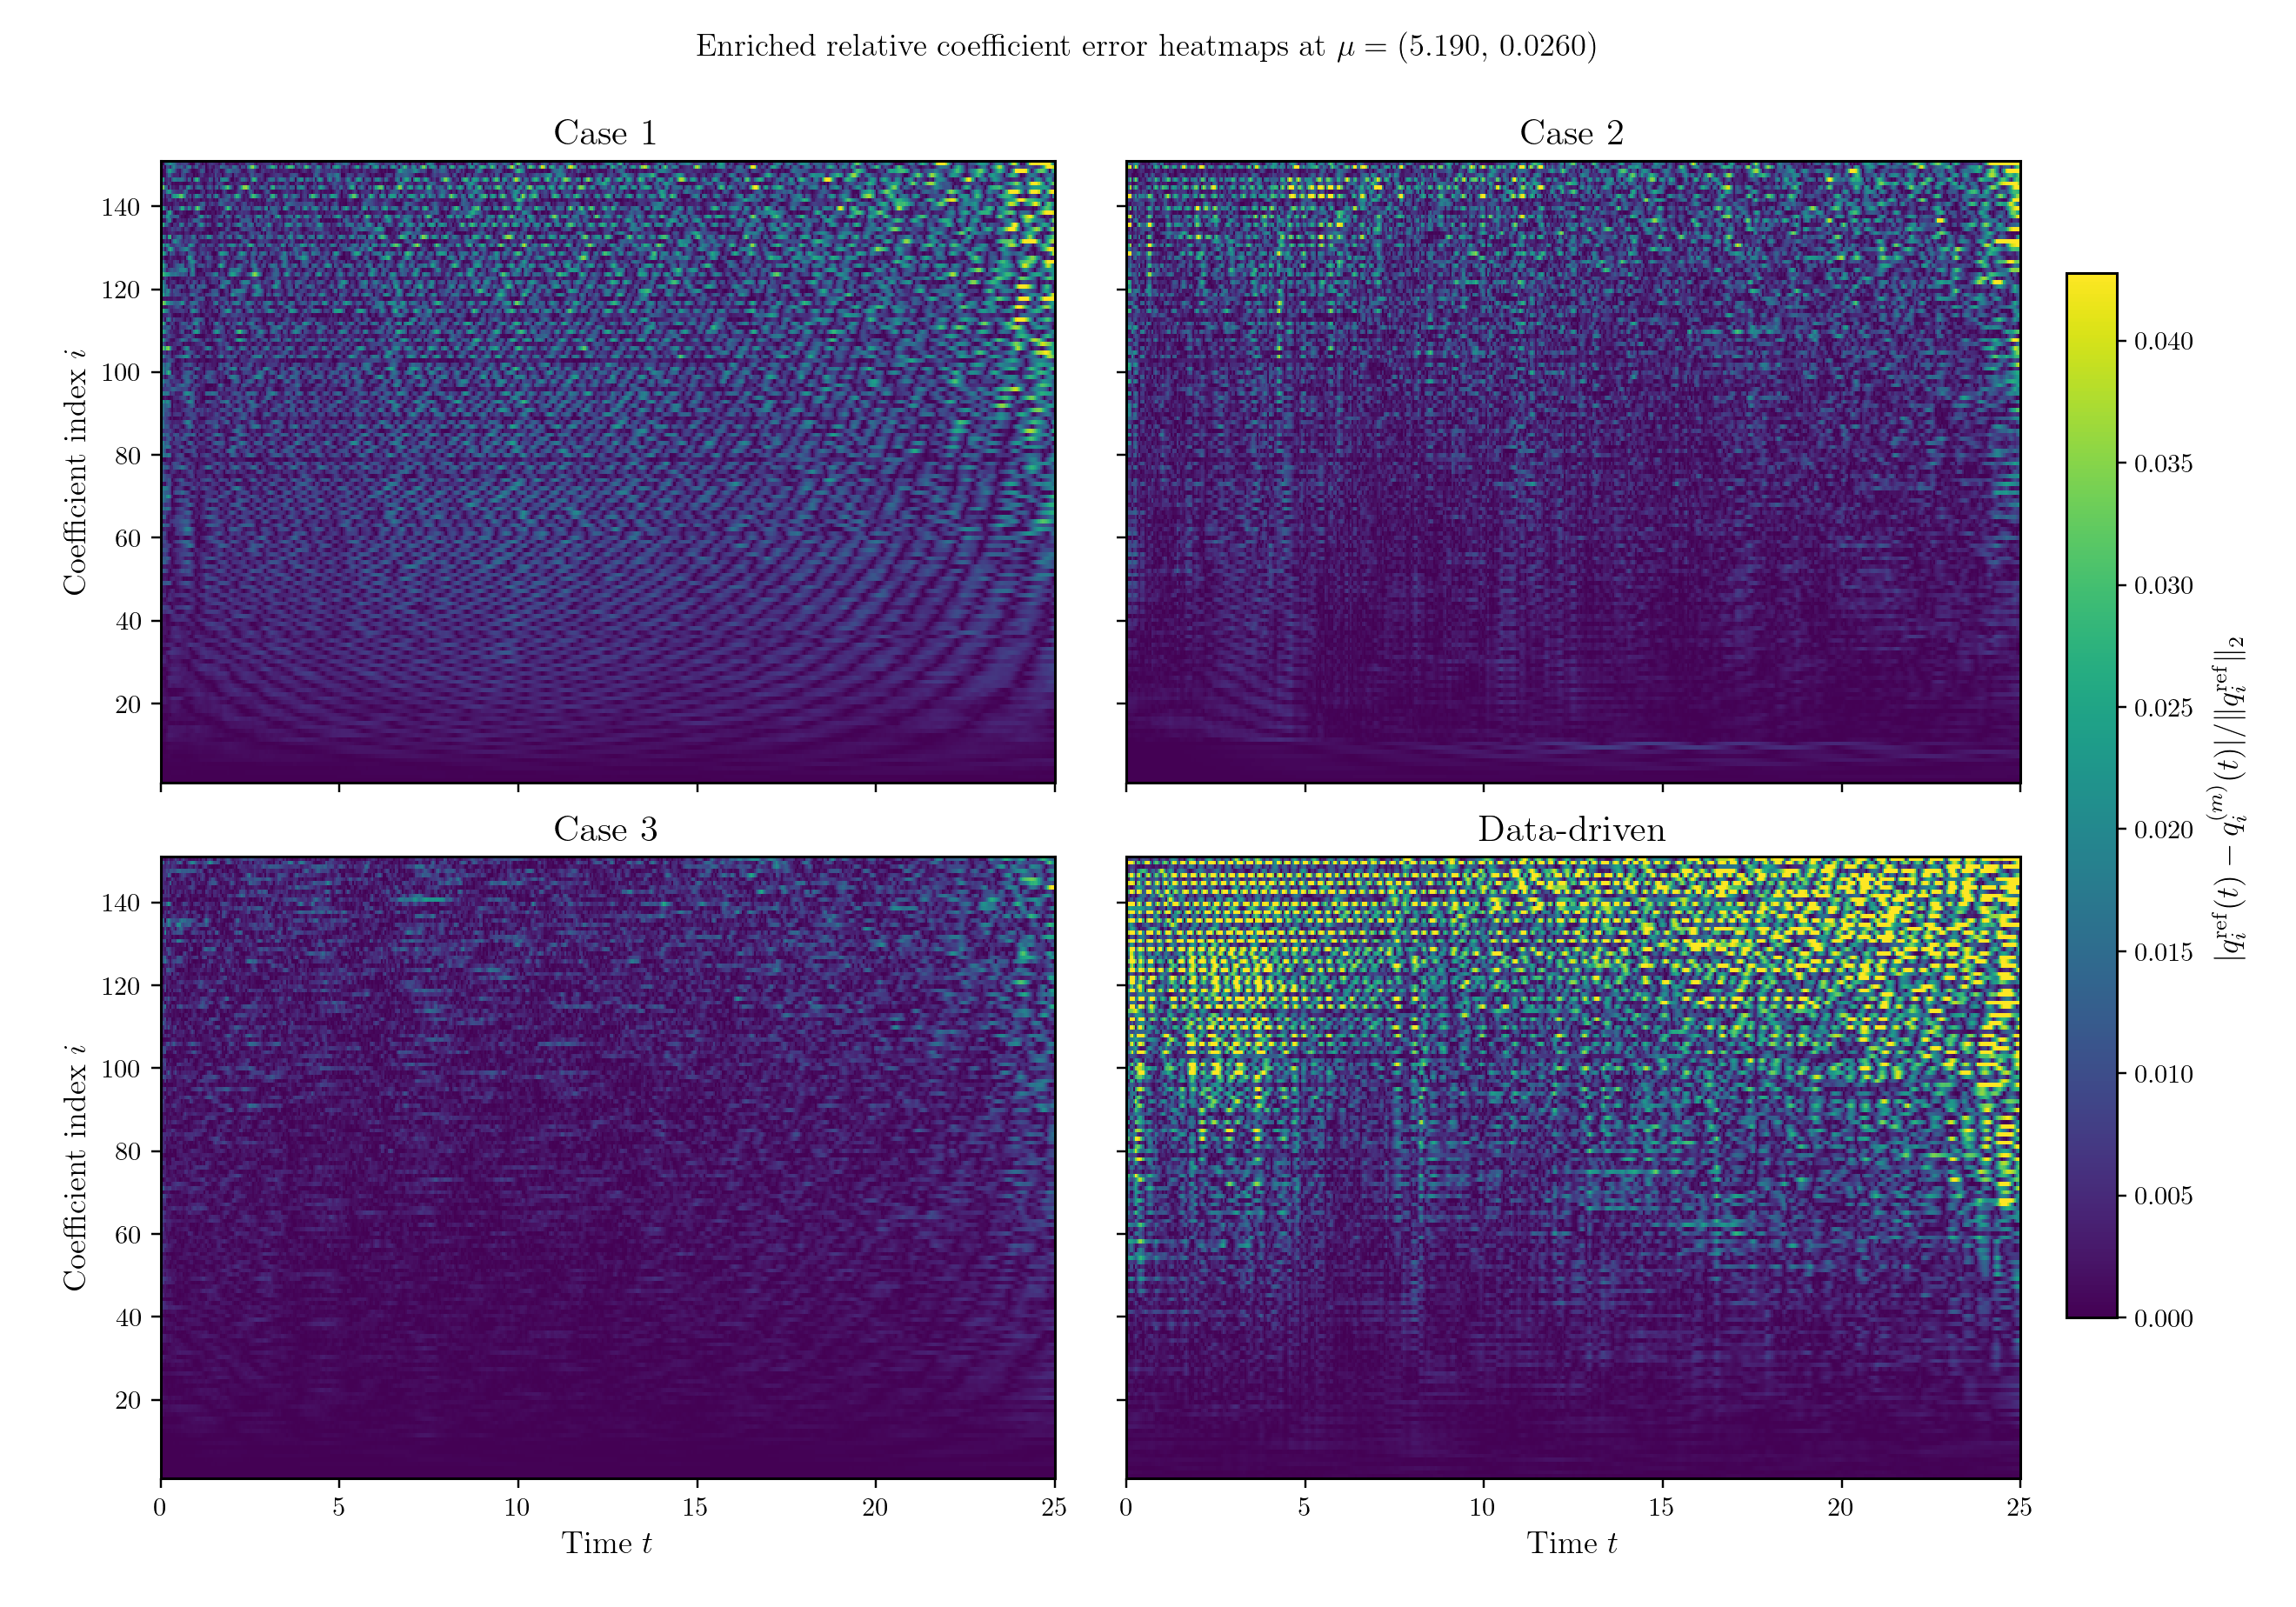
\includegraphics[width=0.98\textwidth]{Figures/coeff_errors/enriched_mu1_5.190_mu2_0.0260_coeff_rel_heatmap_grid.png}
\caption{Enriched stage: relative coefficient error heatmaps at $\bm\mu^{(2)}=(5.19,0.026)$.}
\label{fig:hm_enriched_rel_mu2}
\end{figure}



\bibliographystyle{unsrt}
\bibliography{bibliography}
\end{document}
